\documentclass[%
    paper=A4,                   % paper size --> A4 is default in Germany
    twoside=true,               % onesite or twoside printing
    openright,                  % doublepage cleaning ends up right side
    parskip=full,               % spacing value / method for paragraphs
    chapterprefix=true,         % prefix for chapter marks
    11pt,                       % font size
    headings=normal,            % size of headings
    bibliography=totoc,         % include bib in toc
    listof=totoc,               % include listof entries in toc
    titlepage=on,               % own page for each title page
    captions=tableabove,        % display table captions above the float env
    draft=true,                 % value for draft version
]{scrreprt}%

\usepackage[utf8]{inputenc}
\usepackage[english]{babel}
\usepackage[%
    figuresep=colon,%
    sansserif=false,%
    hangfigurecaption=false,%
    hangsection=true,%
    hangsubsection=true,%
    colorize=full,%
    colortheme=bluemagenta,%
    bibsys=bibtex,%
    bibfile=references,%
    bibstyle=alphabetic,%
]{cleanthesis}
\usepackage{subfiles}
\usepackage{amsmath}
\usepackage{amssymb}
\usepackage[inference]{semantic}
\usepackage{galois}
\usepackage{algpseudocode}
\usepackage{graphicx}
\usepackage{url}
\usepackage{IEEEtrantools}

%\listfiles  % Debug LaTeX Information

\newcommand{\thesisTitle}{Structural Optimization of Numerical Programs}
\newcommand{\thesisName}{Xitong Gao}
\newcommand{\thesisDate}{\today}
\newcommand{\thesisVersion}{0.0.1}

\newcommand{\thesisFirstSupervisor}{George A. Constantinides}
% \newcommand{\thesisSecondSupervisor}{John Smith}

\newcommand{\thesisUniversity}{\protect{Imperial College London}}
\newcommand{\thesisUniversityDepartment}{%
    Department of Electrical and Electronic Engineering}
% \newcommand{\thesisUniversityInstitute}{Institut for Clean Thesis Dev}
\newcommand{\thesisUniversityGroup}{Circuits and Systems Research Group}
\newcommand{\thesisUniversityCity}{London}
\newcommand{\thesisUniversityStreetAddress}{South Kensington Campus}
\newcommand{\thesisUniversityPostalCode}{SW7 2AZ}

\hypersetup{%
    pdftitle={\thesisTitle},    %   - title (PDF meta)
    pdfauthor={\thesisName},    %   - author (PDF meta)
    plainpages=false,           %   -
    colorlinks=false,           %   - colorize links?
    pdfborder={0 0 0},          %   -
    breaklinks=true,            %   - allow line break inside links
    bookmarksnumbered=true,     %
    bookmarksopen=true          %
}

\newcommand{\todo}[1]{\{\{\textbf{TODO:} {#1}\}\}\typeout{TODO: {#1}}}

\newcommand{\eg}{\textit{e.g.}}
\newcommand{\etc}{\textit{etc.}}
\newcommand{\etal}{\textit{et~al.}}
\newcommand{\ie}{\textit{i.e.}}

\DeclareMathOperator{\roundup}{\uparrow^\sharp_\circ}
\DeclareMathOperator{\rounddown}{\downarrow^\sharp_\circ}
\DeclareMathOperator{\fresh}{\mathit{fresh}}
\DeclareMathOperator{\eqstep}{\blacktriangleright}
\DeclareMathOperator{\dom}{\mathrm{Dom}}
\DeclareMathOperator{\area}{\mathrm{Area}}
\DeclareMathOperator{\error}{\mathrm{Error}}
\DeclareMathOperator{\abserr}{\mathrm{AbsError}}
\DeclareMathOperator{\abs}{\mathrm{abs}}
\DeclareMathOperator{\frontier}{\textsc{Frontier}}

\newcommand{\naturalset}{\ensuremath\mathbb{N}}
\newcommand{\realset}{\ensuremath\mathbb{R}}
\newcommand{\floatset}{\ensuremath\mathbb{F}}
\newcommand{\powersetof}[1]{\ensuremath\mathcal{P}\left({#1}\right)}
\newcommand{\intervalset}{\ensuremath\mathbf{Interval}}
\newcommand{\floatintervalset}{\ensuremath\intervalset_\floatset}
\newcommand{\errorset}{\ensuremath\mathbb{E}^\sharp}
\newcommand{\labelset}{\ensuremath\mathbf{Label}}
\newcommand{\exprset}{\ensuremath\mathbf{Expr}}
\newcommand{\varset}{\ensuremath\mathbf{Var}}
\newcommand{\env}[1]{\ensuremath\mathbf{Env}_{#1}}
\newcommand{\eqrel}{\ensuremath\mathbin{\rhd}}
\newcommand{\enter}[1]{\ensuremath{A({#1})}}
\newcommand{\interval}[2]{\ensuremath\left[{#1}, {#2}\right]}
\newcommand{\lattice}[2]{\ensuremath\left<{#1}, {#2}\right>}
\newcommand{\join}{\ensuremath\sqcup}
\newcommand{\meet}{\ensuremath\sqcap}

\newcommand{\marteltrace}{\texttt{martel\_trace}}
\newcommand{\frontiertrace}{\texttt{frontier\_trace}}
\newcommand{\greedytrace}{\texttt{greedy\_trace}}

\begin{document}

% Page count
\pagenumbering{arabic}          % arabic page numbering
\setcounter{page}{1}            % set page counter

% Front matter
% !TEX root = ../thesis-example.tex
%
% ------------------------------------  --> cover title page
\begin{titlepage}
	\pdfbookmark[0]{Cover}{Cover}
	\flushright
	\hfill
	\vfill
	{\LARGE\thesisTitle \par}
	\rule[5pt]{\textwidth}{.4pt} \par
	{\Large\thesisName}
	\vfill
	\textit{\large\thesisDate} \\
	Version: \thesisVersion
\end{titlepage}


% ------------------------------------  --> main title page
\begin{titlepage}
	\pdfbookmark[0]{Titlepage}{Titlepage}
	\tgherosfont
	\centering

	
\includegraphics[width=6cm]{imperial_logo} \\[4mm]
    % {\Large \thesisUniversity} \\[4mm]
	\textsf{\thesisUniversityDepartment} \\
	% \textsf{\thesisUniversityInstitute} \\
	\textsf{\thesisUniversityGroup} \\

	\vfill
	{\LARGE \color{ctcolortitle}\textbf{\thesisTitle} \\[10mm]}
	{\Large \thesisName} \\

	\vfill
	% \begin{minipage}[t]{.27\textwidth}
		% \raggedleft
		% \textit{1. Reviewer}
	% \end{minipage}
	% \hspace*{15pt}
	% \begin{minipage}[t]{.65\textwidth}
		% {\Large \thesisFirstReviewer} \\
		  % {\small \thesisFirstReviewerDepartment} \\[-1mm]
		% {\small \thesisFirstReviewerUniversity}
	% \end{minipage} \\[5mm]
	% \begin{minipage}[t]{.27\textwidth}
		% \raggedleft
		% \textit{2. Reviewer}
	% \end{minipage}
	% \hspace*{15pt}
	% \begin{minipage}[t]{.65\textwidth}
		% {\Large \thesisSecondReviewer} \\
		  % {\small \thesisSecondReviewerDepartment} \\[-1mm]
		% {\small \thesisSecondReviewerUniversity}
	% \end{minipage} \\[10mm]
	\begin{minipage}[t]{.27\textwidth}
		\raggedleft
		\textit{Supervisor}
	\end{minipage}
	\hspace*{15pt}
	\begin{minipage}[t]{.65\textwidth}
		\thesisFirstSupervisor%\ and \thesisSecondSupervisor
	\end{minipage} \\[10mm]
    \begin{minipage}[t]{.8\textwidth}
        {\small
            Submitted in part fulfilment of the requirements for the degree of
            Doctor of Philosophy of Imperial College London and the Diploma of
            Imperial College London
        }
    \end{minipage} \\[10mm]

	\thesisDate \\

\end{titlepage}


% ------------------------------------  --> lower title back for single page layout
\hfill
\vfill
{
	\small
	\textbf{\thesisName} \\
	\textit{\thesisTitle} \\
	\thesisDate \\
	% Reviewers: \thesisFirstReviewer\ and \thesisSecondReviewer \\
	Supervisor: \thesisFirstSupervisor%\ and \thesisSecondSupervisor
	\\[1.5em]
    \textbf{\thesisUniversity} \\
	\textit{\thesisUniversityGroup} \\
	% \thesisUniversityInstitute \\
	\thesisUniversityDepartment \\
	\thesisUniversityStreetAddress \\
	\thesisUniversityPostalCode\ and \thesisUniversityCity
}
                   % INCLUDE: all titlepages
\cleardoublepage

\pagestyle{plain}               % display just page numbers
\pdfbookmark[0]{Abstract}{Abstract}
\chapter*{Abstract}
\label{sec:abstract}
\vspace*{-10mm}

This thesis introduces a new technique, and its associated tool \soap, to
automatically perform source-to-source optimization of numerical programs,
specifically targeting the trade-off among numerical accuracy, latency, and
resource usage as a \acrlong{hls} flow for \acrshort{fpga} implementations.  A
new intermediate representation, \acrshort{mir}, is introduced to carry out
the abstraction and optimization of numerical programs.  Equivalent structures
in \acrshortpl{mir} are efficiently discovered using methods based on formal
semantics by taking into account axiomatic rules from real arithmetic, such as
associativity, distributivity and others, in tandem with program equivalence
rules that enable control-flow restructuring and eliminate redundant array
accesses.  For the first time, we bring rigorous approaches from software
static analysis, specifically formal semantics and \acrlong{ai}, to bear
on program transformation for \acrlong{hls}.  New abstract semantics are
developed to generate a computable subset of equivalent \acrshortpl{mir}
from an original \acrshort{mir}.  Using formal semantics, three objectives
are calculated for each \acrshort{mir} representing a pipelined numerical
program: the accuracy of computation and an estimate of resource utilization
in \acrshort{fpga} and the latency of program execution.  The optimization of
these objectives produces a Pareto frontier consisting of a set of equivalent
\acrshortpl{mir}.  We thus go beyond existing literature by not only optimizing
the precision requirements of an implementation, but changing the structure
of the implementation itself.  Using \soap{} to optimize the structure of a
variety of real world and artificially generated arithmetic expressions in
single precision, we improve either their accuracy or the resource utilization
by up to 60\%.  When applied to a suite of computational intensive numerical
programs from PolyBench and Livermore Loops benchmarks, \soap{} has generated
circuits that enjoy up to a 12$\times$ speedup, with a simultaneous 7$\times$
increase in accuracy, at a cost of up to 4$\times$ more \acrshortpl{lut}.
                % INCLUDE: the abstracts (english and german)
\cleardoublepage

% % !TEX root = ../thesis-example.tex
%
\pdfbookmark[0]{Acknowledgement}{Acknowledgement}
\chapter*{Acknowledgement}
\label{sec:acknowledgement}
\vspace*{-10mm}

\todo{Acknowledgement goes here\textellipsis}
         % INCLUDE: acknowledgement
% \cleardoublepage

\pdfbookmark[0]{Table of Contents}{Table of Contents}

\setcounter{tocdepth}{2}        % define depth of toc
\tableofcontents                % display table of contents
\clearpage

\pdfbookmark[1]{List of Figures}{List of Figures}
\listoffigures
\clearpage

\pdfbookmark[1]{List of Tables}{List of Tables}
\listoftables

\renewcommand*{\glsclearpage}{%
\clearpage\pdfbookmark[1]{List of Acronyms}{List of Acronyms}}%
\printglossary[type=\acronymtype, style=super, title=List of Acronyms]%
\glsresetall%

% Body matter
\pagestyle{maincontentstyle}    % fancy header and footer

% Main text
\chapter{Introduction}
\label{chp:introduction}

As the computational capability of \gls{fpga} devices grows at an exponential
rate, numerical applications running on them become increasingly more
complex.  Traditional design methodologies, working at the \gls{rtl}, have
become increasingly costly, forcing us to work at a higher abstraction
level~\cite{gajski, bdti_xilinx, meeus12}, \eg~to implement our designs using
\glspl{hll} such as C\@.

There are many reasons why \gls{fpga} implementations of numerical algorithms
are now best obtained via \gls{hls} from C\@: less development effort, the
abundance of software engineers compared to hardware designers, the relative
ease of testing C code on an ordinary microprocessor, the opportunities
for rapid design space exploration, and so on~\cite{gajski94, meeus12,
nane15}. Great advances have been made in this area recently, and the
output from \gls{hls} tools is nowadays competitive with hand-crafted
designs~\cite{bdti_xilinx}.

Numerical C programs are typically written with floating-point
arithmetic, following the \emph{IEEE 754 standard} for floating-point
computation~\cite{ieee754}.  Floating-point numbers can represent a wide
range of real values, and most programming languages support the standard
seamlessly.  The standard has become ubiquitous, and is used in most of our
software and hardware implementations of numerical programs.  Recently,
Altera has introduced Arria 10 and Stratix 10 devices to incorporate hardened
floating-point \gls{dsp} blocks in the \gls{fpga} fabric~\cite{stratix10fp}.
As a result, we expect to see floating-point arithmetic continuing to dominate
in the \gls{fpga} implementation of numerical applications.

Although we make use of floating-point arithmetic to implement algorithms,
generally specified in real arithmetic, in practice, it is often neglected that
floating-point computations almost always have \emph{round-off errors}, \ie~the
discrepancy between the actual result in real arithmetic and the rounded result
computed with floating-point arithmetic.  Round-off errors, when accumulated,
can have a devastating effect on numerical accuracy~\cite{higham02}.

In fact, properties such as associativity $(a + b) + c \equiv a + (b +
c)$ and distributivity $a \times (b + c) \equiv a \times b + a \times c$
which we consider to be fundamental laws of real numbers no longer hold
under floating-point arithmetic~\cite{goldberg}.  For instance, under
single-precision floating-point arithmetic with rounding to the nearest, the
result of $(2^{-24} + 2^{-24}) + 1 = 1.00000012\mathellipsis$ is exact, but
$(1 + 2^{-24}) + 2^{-24}$ is rounded to $1$.  Round-off errors in a numerical
program are dependent on every arithmetic operation and every input value, and
with the impact on floating-point accuracy being so esoteric, it is challenging
for engineers to understand the repercussions of switching between
``\verb|(a + b) * c|'' and ``\verb|a * c + b * c|'' in their programs.

These numerical properties nevertheless open the possibility of using these
rules to generate a program equivalent to the original program in real
arithmetic, but which could have better quality than the original when
evaluated in floating-point computation.  Experienced engineers often apply
such expression rewriting intuitions in numerical programs.  For instance, when
summing a sequence of floating-point values, one can sometimes reduce round-off
error in the result by summing the inputs in ascending order of magnitude.
On the other hand, one can often reduce latency by applying \emph{expression
balancing}, \ie~rearranging operators in an expression to construct a balanced
tree, so that more operators can work in parallel.  These heuristics cover a
very limited number of possible transformations and may not always improve
the original code.  There does not exist a trivial process to apply steps of
transformations using equivalence rules to \emph{optimally} trade off latency,
resources and numerical accuracy.

Existing \gls{hls} tools consider these rewrites to be
unsafe~\cite{vivado_hls}, and thus make very limited use of them
when restructuring floating-point data-paths.  For instance,
\gls{vhls}~\cite{vivado_hls} has only a very simple \emph{expression balancing}
feature that uses associativity to improve latency, and only expressions with
either additions or multiplications are optimized.  Moreover, it does not
produce optimal loop pipelining, because it does not take into account the
implications of these transformations on inter-iteration dependences and does
not explore partial loop unrolling.  In addition, \gls{vhls} cannot reason
about how this feature affects numerical accuracy; there is no guarantee
that this transformation will not result in a catastrophically inaccurate
implementation.

In response, this thesis proposes new methodologies and an associated
tool---\soap, a fully automatic source-to-source optimizer that augments
\gls{vhls}---to optimize a given numerical C program using these
transformations in tandem with conventional program transformations.  The
optimizer discovers not only one, but a wide spectrum of program candidates.
When synthesized in \gls{vhls}, these candidates trade off three performance
metrics of great importance to engineers: run time, resource usage and
round-off error.  Here, run time refers to the latency in clock cycles,
resource usage refers to the number of \glspl{lut} and \gls{dsp} elements.
Some of these performance metrics could be in conflict.  For example, higher
performance tends to require more circuitry, and how to resolve this trade-off
depends on the user's requirements.  As a result, the tool produces a
\emph{set} of optimized programs, known as the \emph{Pareto frontier}: those
programs $P$ for which the tool has found no $P'$ that improves on $P$ in all
three metrics.  We thus go beyond existing literature by not only optimizing
the precision requirements of an implementation, but changing the structure of
the implementation itself.

The program optimization flow is \emph{safe} and \emph{semantics-directed}.
\emph{Safety} means that because we base our method on formal mathematics to
optimize programs, our approach can be proved correct, in the sense that when
executed using exact real arithmetic, the transformed version produces exactly
the same output values as the original program. \emph{Semantics-directed}
transformation means that not only do we use program syntax, but also the
semantics, \ie~the underlying meaning of programs such as inferred numerical
accuracy, to guide optimization and guarantee safety properties of the
optimized program.  Our technique obtains when necessary, by analyzing the
program, a bound and a round-off error bound on each variable in every program
location.  These information are then used to guide program optimization, by
analyzing and manipulating not only the syntax, but also the semantics of
programs.

Generating candidate optimizations na{\"\i}vely would however produce a
combinatorial explosion, even for small input programs.  For instance, in the
worst case, the parsing of a simple summation of $n$ variables could result
in $(2n - 3)!! = 1 \times 3 \times 5 \times \cdots \times (2n - 3)$ distinct
expressions modulo commutativity, \ie~we make use of associativity but ignore
any distinction caused by commutativity~\cite{ioualalen, mouilleron}.  This is
further complicated by distributivity as the expression ${(a + b)}^k$ could
expand into an expression with a summation of $2^k$ terms each with $k - 1$
multiplications.  Usually, for this reason, it would be infeasible to generate
a complete set of equivalent expressions using the rules of equivalence, since
an expression with a moderate number of terms will have a very large number of
equivalent expressions, and this number grows faster than exponential rate with
the increase of the number of terms.  New approaches were therefore developed
specifically to tackle the efficient discovery of equivalent structures in
numerical programs.  First, we invent a new intermediate representation,
called \gls{mir} to reduce the size of our search space without affecting its
optimality.  Second, we further reduce the effort of exploring the new search
space by intelligently pruning the set of candidates as it progresses up the
input program's abstract syntax tree.

All of the techniques above are designed with \emph{compositionality} in mind.
This means that we recursively break down each component we work on---such
as programs and \glspl{mir}---into smaller components and use our analyses
to calculate the results of each, such as accuracy, area and latency, and
subsequently equivalent candidates; the final results are then constructed from
those of the subcomponents.  When compared with a global approach, there are
two major advantages.  First, because components are considered independent
of each other, once analyzed the results can be reused in the analysis in the
larger enclosing components.  Another advantage of this is that although we
will not formally prove the correctness of the methodologies in this thesis,
they are designed to be easily expressible in a formal language, and by proving
small lemmas, we can deductively prove the correctness of, for instance, a
program-to-\gls{mir} translation.

\section{Thesis Organization}
\label{intro:sec:organization}

Chapter~\ref{chp:background} serves to explain various essential concepts
used throughout this thesis.  Our techniques discussed in this thesis
naturally extends \gls{hls}, a process to compile a program written in
high-level languages such as C into circuits.  We therefore start by
introducing the advantages of \gls{hls}, compared against manual \gls{rtl}
implementations.  We then bring rigorous approaches from software static
analysis, specifically program semantics and abstract interpretation, to
source-to-source transformation for \gls{hls}\@.  We introduce existing
intermediate representations designed for program optimizations, and highlight
the advantages and disadvantages of them relevant to our requirements.  We
draw comparisons between others' work and ours to better motivate the thesis's
contributions.  We further explain existing program rewriting techniques for
numerical accuracy, which inspired our efficient discovery of equivalent
programs.  Finally, we introduce the concept of loop pipelining and how
restructuring numerical programs can optimize run time.

In Chapter~\ref{chp:stropt} we propose new methods to automatically optimize
the structure of arithmetic expressions for \gls{fpga} implementation as part
of a high-level synthesis flow.  This chapter introduces the basis of the
practice we use to perform structural optimization on numerical programs,
taking into account axiomatic rules derived from real arithmetic, such as
distributivity, associativity and others.  A new efficient method is proposed
to generate a computable optimized subset of equivalent expressions from an
original expression.  Our approach explicitly target an optimized area/accuracy
trade-off, by automatically rewriting arithmetic expressions, and analyzing
each expression rewritten for its accuracy and area usage.  This gives
the synthesis tool the flexibility to choose an implementation satisfying
constraints on both accuracy and resource usage.  Using our technique to
optimize the structure of a variety of real world and artificially generated
examples in single-precision, we improve either their accuracy or the resource
utilization by up to 60\%.

Chapter~\ref{chp:progopt} presents a similar source-to-source optimization
targeting the trade-off between numerical accuracy and resource usage,
but we have extended it to optimize general numerical programs, including
\iflit~statements and \whilelit~loops.  Because there are infinite number
of ways to rewrite numerical C programs, and many of these rewrites produce
programs that have the same resource usage, accuracy and latency properties, we
propose a novel expression-based intermediate representation called \gls{mir}
to reduce the number of rewrites to explore.  In Chapter~\ref{chp:progopt}
we explain in detail the structure of \glspl{mir}, and the back-and-forth
translation between numerical C programs and \glspl{mir}.  We efficiently
discover equivalent structures in \glspl{mir} by exploiting not only the rules
of real arithmetic, such as associativity and distributivity, but also rules
that enable control-flow restructuring.  Our numerical accuracy and resource
usage analyses are further extended to analyze \glspl{mir}.  Additionally, we
broaden the Pareto frontier in our optimization flow to automatically explore
the numerical implications of partial loop unrolling and loop splitting.  In
real applications, the tool discovers a wide range of Pareto optimal options,
and the most accurate one improves the accuracy of numerical programs by up to
65\%.

The optimization techniques we have discussed so far have only been limited
to minimizing area and round-off errors of numerical programs.  Often such
optimizations result in programs with longer run time, yet there are potentials
for these transformations to significantly reduce the run time of numerical
programs while improving resources and accuracy.  In Chapter~\ref{chp:latopt},
we therefore introduce a new analysis procedure to minimize yet another
objective: the total run time of the optimized program.  Together with accuracy
and resource utilization, these three form the simultaneous goals we use
to produce the Pareto frontier.  In this chapter, \glspl{mir} are extended
with new operators to allow for arrays and matrices in the source program,
to optimize a wide-range of practical numerical applications.  Numerical
programs typically spend most of their run time in loops, so state-of-the-art
\gls{hls} tools use pipelining to schedule them efficiently.  Still, the run
time performance of the resultant \gls{fpga} implementation is limited by data
dependences between loop iterations.  We thus present additional rewriting
rules---memory access reductions---along with arithmetic identities and
control-flow transformations to alleviate some of these dependence constraints.
\gls{hls} tools cannot safely enable such rewrites by default because they may
impact the accuracy of floating-point computations and increase area usage,
whereas we optimize run time while controlling the implications on accuracy and
area.  Again, the tool reports a multi-dimensional Pareto frontier that the
programmer can use to resolve the trade-off according to their needs.  When
applied to a suite of PolyBench and Livermore Loops benchmarks, the tool has
generated programs that enjoy up to a 12$\times$ speedup, with a simultaneous
7$\times$ increase in accuracy, at a cost of up to 4$\times$ more \glspl{lut}.

Finally, Chapter~\ref{chp:conclusion} concludes this thesis by summarizing
our research, and we discuss the potential for how future research into the
structural optimization of numerical programs could further benefit the
high-level synthesis community.

\section{Contributions}
\label{intro:sec:contributions}

In this section, we summarize the following original major contributions in
this thesis:
\begin{itemize}

    \item a new expression-based \gls{ir}, \acrfull{mir}, developed based on
    the formal semantics of programs, to safely and considerably reduce the
    size of the search space of equivalent programs~\cite{soap2};

    \item an efficient algorithm to discover equivalent expressions and
    \glspl{mir} through bottom-up hierarchy, graph partitioning, and
    intelligent pruning of optimization candidates by performing accuracy, area
    estimation and latency analysis~\cite{soap};

    \item we bring together standard program equivalences that do not affect
    program behavior (\eg~loop/branch splitting/merging, partial loop
    unrolling, rules that removes extraneous array accesses), and non-standard
    transformation rules (\eg~arithmetic rules), to be used in a novel way to
    significantly impact latency, resource usage and accuracy of a numerical
    program~\cite{soap3};

    \item an accuracy analysis based on abstract interpretation to calculate
    bounds on the output and their corresponding round-off errors of a given
    optimized expression~\cite{soap} or program candidate~\cite{soap2};

    \item a scheduling analysis that estimates the latency and resource usage
    of a given optimized candidate~\cite{soap3}; and

    \item incorporating the above-mentioned techniques, the first optimizer
    to \emph{automatically} and \emph{safely} produce optimized programs
    (and subsequent \gls{rtl} implementations with \gls{vhls}) on the
    three-dimensional Pareto frontier of options that trade off run time,
    accuracy, and area~\cite{soap3}.

\end{itemize}

\section{Publications}
\label{intro:sec:publications}

\begin{itemize}
    \item
        Xitong Gao, Samuel Bayliss, and George A. Constantinides.
        ``\emph{SOAP\@: Structural Optimization of Arithmetic Expressions
        for High-Level Synthesis}''. In 2013 International Conference on
        Field-Programmable Technology (FPT). 2013, pp. 112–119.

    \item
        Xitong Gao and George A. Constantinides. ``\emph{Numerical Program
        Optimization for High-Level Synthesis}''. In Proceedings of the
        2015 ACM/SIGDA International Symposium on Field-Programmable Gate
        Arrays. 2015, pp. 210–213.

    \item
        Xitong Gao, John Wickerson, and George A. Constantinides.
        ``\emph{Automatically Optimizing the Latency, Area, and Accuracy
        of C Programs for High-Level Synthesis}''. In Proceedings of the
        2016 ACM/SIGDA International Symposium on Field-Programmable Gate
        Arrays. 2016, pp. 234–243.
\end{itemize}



\chapter{Background}
\label{chp:background}

\section{Introduction}

Our previous chapter introduced a new methodology to efficiently restructure
arithmetic expressions for the optimized trade-off between two performance
metrics, \ie~numerical accuracy when evaluated and area usage in synthesized
FPGA implementations.  However, this method has a substantial limitation when
applied to general numerical programs, that is, it can only be applied to
straight-line codes without control structures such as branches and loops.

The structural optimization of general numerical programs is much more complex
than that of arithmetic expressions.  The reasons are two-fold.  First,
during program execution, variables are often updated with new values.  Our
optimization should therefore perform static analysis on the values of
variables, and use the result to optimize specifically for the trade-off
between accuracy and resource usage.  Second, it is much more difficult to
formally define program equivalence, and subsequently, to search efficiently
for optimized equivalent programs.  For instance, even without the introduction
of branches and loops, the following two programs are equivalent, but
syntactically, they are very different.  In practice, it is desirable to
eliminate as much as possible the need for these syntactic rewrites that do not
affect our performance metrics.

\begin{figure}[ht]
    \centering
    \subfloat[$P_1$]{%
        \shortstack[l]{%
            \texttt{x = x + 1;} \\
            \texttt{y = 2 * x;} \\
            \texttt{x = x + 3;}
        }
    } \qquad \qquad
    \subfloat[$P_2$]{%
        \shortstack[l]{%
            \texttt{y = x + 1;} \\
            \texttt{x = y;} \\
            \texttt{y = y * 2;} \\
            \texttt{x = x + 3;}
        }
    }
    \caption{Two programs that are equivalent but syntactically different.}
    \label{fig:equiv_progs}
\end{figure}

Therefore, in this chapter, we provide answers to these two above issues.  In
the meantime, we propose a new general \emph{program} optimization technique
for numerical algorithms, which allows \texttt{if} statements as well as
\texttt{while} loops, and developed its accompanied tool, \newsoap, to enable
the joint optimization of accuracy and resource usage, as well as the trade-off
between these performance metrics.  We develop a tool, which we call \newsoap,
to perform source-to-source optimization of numerical programs targeting FPGAs,
and generate implementations that trade off resource usage and numerical
accuracy.

% floating-point arithmetic has round-off errors, exploit equivalence

Similar to the approach we have proposed in Chapter~\ref{chp:stropt}, we
exploit equivalence rules such as such as \emph{associativity} $(a + b) +
c \equiv a + (b + c)$, and \emph{distributivity} $(a + b) \times c \equiv
a \times c + b \times c$ to automatically optimize implementations for
the optimal trade-off between resource usage, \ie~the number of LUTs and
DSP elements utilized, and accuracy when evaluated using floating-point
computations.  For example, with single precision floating-point format, our
tool found that give an input $x \in [0, 100]$ and $y \in [0, 2]$, then the
program:
\begin{lstlisting}
    if (x < 1) {
        x = (x + y) + 0.1;
    } else {
        x = x + (y + 0.1);
    }
\end{lstlisting}
is most accurate when rewritten in the following form:
\begin{lstlisting}
    if (x < 1) {
        x = (x + 0.1) + y;
    } else {
        x = x + (y + 0.1);
    }
\end{lstlisting}
On the other hand, the original program uses fewest resources when
subexpressions are shared and the \iflit~statement is eliminated:
\begin{lstlisting}
    x = x + (y + 0.1);
\end{lstlisting}

This kind of optimization generates a Pareto optimal set of implementations,
which trades off accuracy and area.  A na{\"\i}ve strategy to search for
the Pareto optimal implementations is to discover all possible equivalent
expressions.  However, this would result in combinatorial explosion and become
intractable even for very small expressions~\cite{ioualalen,mouilleron}.  To
remedy this, in Chapter~\ref{chp:stropt} we proposed a novel approach, known
as \soap, to significantly reduce the space and time complexity to produce a
subset of the Pareto frontier.

% program transformation why?

Our program optimization flow is \emph{safe}, \emph{semantics-directed} and
\emph{flexible}. \emph{Safety} means that because we make use of formal
mathematics to optimize programs, our approach can be proved correct, in
the sense that when executed using exact real arithmetic, the transformed
version produces exactly the same output values as the original program.
\emph{Semantics-directed} transformation means that not only do we use
program syntax, but also the semantics to guide optimization and guarantee
safety properties of the optimized program.  Our technique obtains when
necessary, by analyzing the program, a bound and a round-off error bound on
each variable in every program location.  These information are then used
to guide program optimization.  By analyzing and manipulating not only the
syntax, but also the semantics of programs.  The meaning of a \emph{flexible}
program transformation is three-fold.  First, arithmetic computations can be
optimized across assignments, \iflit~statements and \whilelit~loops.  Secondly,
we automatically explore the numerical implications of partial loop unrolling
and loop splitting, which can create more opportunity for minimizing round-off
errors, hence further increases range of options in the Pareto frontier of
trade-offs.  Finally, our method naturally subsumes constant propagation,
redundant code elimination, and also branch and loop fusions.

% Our tool fits in the familiar setting of the high-level synthesis tool flow, as a front-end that performs the source-to-source optimization of

Our main contributions in this chapter are as follows:
\begin{enumerate}
    \vspace{-6pt}
    \item
        A new intermediate representation of the behaviour of numerical
        programs, its structure is designed to be manipulated and analyzed
        with ease.  A new framework of numerical program transformations is
        developed to enable the back and forth translation between the program
        and a new intermediate representation (IR), which preserves the
        semantics of the original program.
    \vspace{-6pt}
    \item
        Semantics-based analyses that reason about not only the resource
        utilization (number of LUTs and DSP elements), and safe ranges of
        values and errors for programs, but also potential errors such as
        overflows and non-termination.
    \vspace{-6pt}
    \item
        A new tool, \newsoap, which trades off resource usage and accuracy
        by providing a safe, semantics-directed and flexible optimization
        targeting numerical programs for high-level synthesis.
    \vspace{-6pt}
\end{enumerate}

Section~\ref{sec:related_work} provides an overview of the existing work
related in both the software and high-level synthesis community.  We then
proceed to define our program syntax in Section~\ref{sec:syntax_definition}.
Using the syntax definition, we provide a detailed formal explanation
of our numerical program transformation, which consists of three
stages.  Section~\ref{sec:program_to_mir}, {}~\ref{sec:transformations},
{}~\ref{sec:code_generation} describe in sequence how numerical programs
can be translated into MIRs, how we infer bounds and error bounds on
variables and analyze resource usage estimates for the efficient discovery
of equivalent structures in the analyzed MIR, and finally, we explain how
a chosen MIR can be translated into an optimized numerical program.  Then
we present the optimization results in Section~\ref{sec:results} and
Section~\ref{sec:conclusion} concludes this chapter.

\section{Field-Programmable Gate Arrays}
\label{bg:sec:fpga}

\subsection{Computing Architectures}
\label{bg:sub:computing_architectures}

When it comes to implementing computations, we often choose from a
spectrum of computing machines.  These choices range from ones with fixed
architectures that computes by executing \emph{software} designs, such as
CPUs and general-purpose graphics processing units (GPUs), to ones that can
implement custom \emph{hardware} architectures, such as FPGAs and ASICs
(application-specific integrated circuits).

There has been a great amount of efforts in recent decades to make
fixed-architecture machines run as fast as possible; many novel and intricate
ideas were proposed and we now have many general circuitries in CPUs to
improve their performance~\cite{comparch}.  For instance, CPUs could have a
pipeline that spans several clock cycles to fetch and decode instructions,
access data from memory or registers to carry out computations.  At the same
time, they would make predictions about the branches taken in control-flows,
as the pipeline must be flushed if an incorrect instruction is fetched,
incurring a penalty in speed.  They could also exploit instruction-level,
data-level and thread-level parallelism, in order to maximize opportunities to
parallelize computations.  These are just the tip of the iceberg, as many other
architectural advancements exist.

The great majority of fixed-architecture computing machines are based on
\emph{von Neumann architecture}, which consists of three parts: a computation
unit, a memory and a bus between them to move data back and forth.  Often
applications running on these machines could spend a majority of their time
and energy to move data and instructions in the memory from/to the right
location in the processor as fast as possible, in order to carry out arithmetic
computations.  Because computational tasks frequently reuse input data and
intermediate results, a hierarchy of caches, in tandem with cache-aware
compiler optimizations~\cite{kowarschik03}, are often used to mitigate the
costs of exchanging data between the processor and the memory.  Despite
these optimization efforts to run software code as fast as possible, the
processor-memory bus, which is often referred to as the \emph{von Neumann
bottleneck}~\cite{backus78}, inherently exist and it remains the limiting
factor of performance in the architecture, and this phenomenon is known to many
as \emph{hitting the memory wall}~\cite{bacon13, wulf94}.

Custom architectures in general achieve much higher performance, thanks to
their ability to implement arbitrary digital circuits specifically designed for
the application under consideration, and spatially distribute memory bandwidth
and computations.  This is in stark contrast to microprocessors such as CPUs
and GPUs, which utilize general-purpose circuitry to cope with a wide-range
of applications.  ASICs provide the best power efficiency and performance
among all above architectures, however they are often associated with long
development cycles and high costs; any updates to the design would require a
complete and expensive re-spinning of the circuits~\cite{bacon13}, as they
are inherently non-programmable.  FPGAs provide the best trade-off between
processors and ASICs.  Not only do FPGAs have better performance and power
characteristics than fixed architectures, they also offer high programmability
which makes FPGAs cost-effective low-volume ASIC replacements~\cite{karen04,
bacon13}.  At the same time, with a much shorter development period than ASICs,
hardware designs on FPGAs can be implemented with a much lower cost, and
shorter time to market enables a substantially larger profit by a competitively
early market entry~\cite{semico12}.  For the above reasons, being able to
expose parallelism from bit-level all the way to the loop and task level, FPGAs
have been increasingly used as high-performance and low-power alternatives to
CPUs and GPUs for many classes of applications~\cite{bacon13, brodtkorb10,
sirowy08}.  For example, Thomas~\etal~\cite{thomas09} reported a FPGA-based
random number generator can obtain a $260\times$ speed-up, while costing less
than 1\% of energy to produce each random sample when compared to its software
counterpart running on a CPU\@.  Microsoft embedded Stratix V FPGAs in their
data center, reducing the latency of their Bing web search engine by a factor
of 95\%~\cite{catapult}.


\subsection{FPGA Architecture}
\label{bg:sub:fpga_architecture}

FPGAs owe their high performance and power efficiency to the design of the
architecture, we thus use Altera Stratix V~\cite{stratix5} as an example to
explain the architecture.  Stratix V fabric contain of an two-dimensional array
of logic array blocks (LABs).  Each LAB consists of an array of 10 adaptive
logic modules (ALMs); Figure~\ref{bg:fig:alm} shows a high-level block diagram
of an ALM in Stratix V.  In an ALM, multiplexers can be configured to choose
whether full adders and registers are used.  Dedicated full adders enable more
complex boolean functions to be implemented in a single ALM, whereas the use of
registers, which store intermediate values, determines whether the circuit is
combinational or sequential.  The two look-up tables (LUTs) in an ALM can be
configured to compute a combination of two arbitrary boolean functions, each
with up to 5 inputs from 8 inputs in total.  Stratix 10, slated to be released
in the next couple of years, has up to 1.87 million ALMs and 7.47 registers in
total for the most demanding applications~\cite{stratix10stat}.  Interconnects,
another class of key configurable resources on FPGAs, enable the inputs and
outputs of ALMs to be wired, in order to form larger and complete circuits from
the two-dimensional array of ALMs.  This allows the FPGA fabric to realize
arbitrary digital circuits.
\begin{figure}[ht]
    \centering
    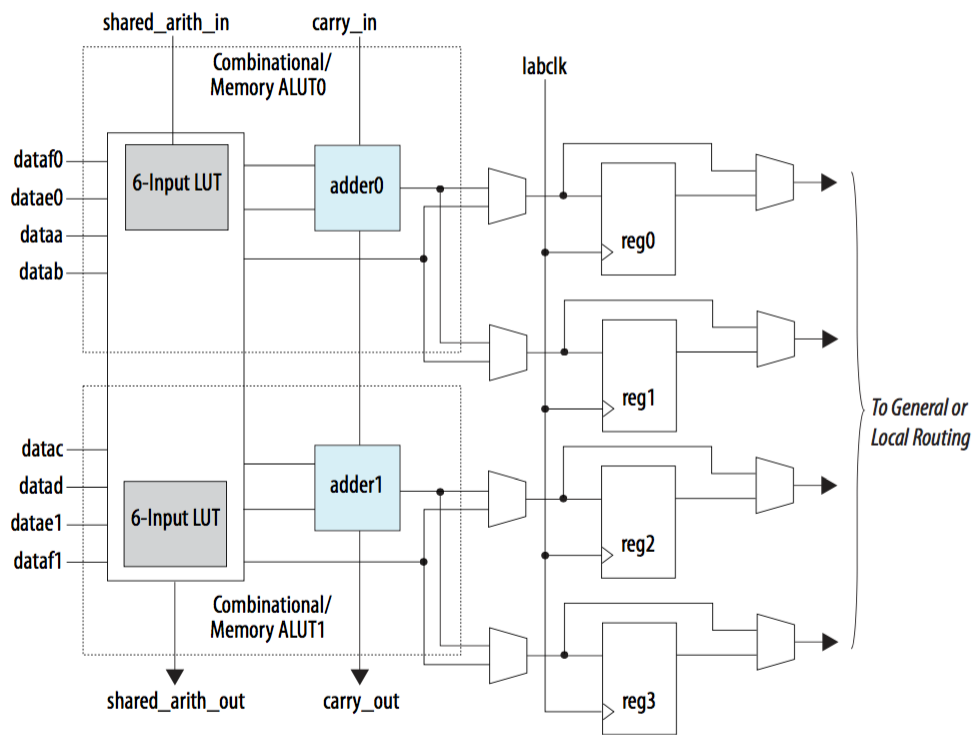
\includegraphics[width=0.8\linewidth]{bg/fig/alm.png}
    \caption{%
        A high-level block diagram of an ALM in Stratix V, from Stratix V
        Device Handbook~\cite{stratix5}.
    }\label{bg:fig:alm}
\end{figure}

% distributed memory and DSP elements

FPGAs with enough ALMs and interconnects can implement arbitrary digital
designs.  This versatile architecture therefore overcomes the memory wall
problem by not restricting itself to von Neumann architecture.  In contrary,
as we have mentioned earlier, while CPUs have general-purpose circuitries that
perform well across a range of applications, FPGAs can implement a circuit that
is individually tailored for the application.  Moreover, unlike the CPU which
only have a small set of registers, the FPGA with its flexibility and abundant
registers, allows designs to place memory and computation units in close
proximity.

Traditionally, multipliers, when implemented in FPGAs, cost a large number of
ALMs.  Stratix devices thus further include an array of hardened components
to carry out arithmetic operations distributed on the FPGA fabric, known as
\emph{digital-signal processing} blocks (DSPs, or simply DSPs).  Because
of the dedicated hardened circuits, DSPs compute faster than arithmetic
operators formed by ALMs only, meanwhile they free ALM resources to perform
more non-arithmetic computations.  In Stratix V, each variable-precision
DSP is paired with a LAB\@.  These DSPs, can be configured in
combinations to perform a wide variety of arithmetic operations, ranging from
using a single DSP element to synthesize three multipliers with two 9-bit
inputs, up to combining four DSPs to form a complex-number multiplier
with two 27-bit inputs~\cite{stratix5}.  Computations with larger inputs can
also be implemented by using ALMs and DSPs to form larger arithmetic
circuits.  Finally, Stratix 10 will further introduce hardened floating-point
DSPs, enabling IEEE 754~\cite{ieee754} single-precision floating-point
additions and multiplications, achieving a performance of up to 10 tera
floating-point operations per second (TFLOPS)~\cite{stratix10fp}.  These DSP
blocks can also be adapted to multiply fixed-point inputs.

DSPs accelerate arithmetic computations, however they need to be supplied
with inputs as fast as they can process to fully utilize them.  Fortunately
in general, in most applications, data are frequently reused by the same
computation unit.  Stratix V therefore include dedicated embedded memory called
M20K blocks (20 Kb storage) that can be arranged and combined into dual-port
RAMs.  Half of the LABs on the device, called MLABs can also be configured to
become a 640-bit RAMs.  These memory blocks are distributed across the FPGA
fabric, so that DSPs can find them in proximity.


\subsection{RTL Design}
\label{bg:sub:rtl_design}

Modern FPGAs---with up to several million LUTs, and thousands of
embedded memory and DSP blocks, wired through a programmable fabric of
interconnects---are humanly intractable to program at the granularity of these
individual components~\cite{kapre08}.  FPGA applications therefore are commonly
written in register-transfer level (RTL) hardware descriptions.

\section{High-Level Synthesis}
\label{bg:sec:high_level_synthesis}

High-level synthesis (HLS) is the process of compiling a high-level
representation of an application (usually in C, C++ or MATLAB) into a
register-transfer-level (RTL) implementation~\cite{coussy, gajski}.  In turn,
this RTL design can be synthesized into a circuit and programmed onto the FPGA
device.

The major advantage of HLS tools is that they enable us to work in a high-level
language (HLL), as opposed to facing labor-intensive tasks such as optimizing
timing and designing control logic in the RTL design process.  This allows
application designers to focus instead on the algorithmic and functional
aspects of their implementation~\cite{coussy}, without concerning themselves
with the above intricate details of manual RTL designs.

Another advantage of using HLS tools is that they are in general more
productive and less error-prone to work with, when compared with traditional
RTL tools.  The reasons are two-fold.  First, a C description is smaller than
a traditional RTL description by a factor of 10~\cite{coussy, bdti}.  Second,
RTL design can be notoriously difficult to debug, whereas C code can be easily
tested on an ordinary microprocessor, and mature debug and analysis tools for C
are freely accessible~\cite{canis13}.

HLS tools further benefit us in their ability to automatically search
the design space with a reasonable design cost~\cite{bdti}, potentially
explore a large number of trade-offs between performance, cost and
power~\cite{mcfarland}, which is generally much more difficult to achieve
in RTL tools.  Our thesis proposes a natural extension to HLS tools by
automatically exploring the space of rewrites of floating-point numerical
C programs, which are equivalent in real arithmetic, but could trade off
accuracy, throughput and resource utilization when synthesized into circuits.

With recent advancements in this area, HLS tools has received a resurgence of
interest, particularly in the FPGA community, and some applications synthesized
with HLS tools are now with similar performance when compared with hand-crafted
RTL implementations~\cite{bdti}.  Xilinx now incorporates a sophisticated HLS
flow into its Vivado design suite~\cite{vivado_hls} and the open-source HLS
tool, LegUp~\cite{legup}, is gaining significant traction in the research
community.


\subsection{HLS Design Flow}
\label{bg:sub:hls_design}

In this section, we provide an overview of the stages taken by HLS tool to
compile a C program into RTL implementation, by using LegUp~\cite{legup,
canis13} as our example.  LegUp is an HLS tool which compiles programs to run
on a hybrid software/hardware architecture, and its design flow is shown in
Figure~\ref{bg:fig:legup}, which consists of three major stages to be explained
below.
\begin{figure}[ht]
    \centering
    \includegraphics[width=0.7\linewidth]{bg/fig/legup}
    \caption{%
        The LegUp design flow, adapted from~\cite{canis13} and~\cite{legup}.
    }\label{bg:fig:legup}
\end{figure}

The first stage is to determine which parts of an application on the
function-level are suitable candidates to be synthesized into hardware
circuits, whereas the others can be run on a processor.  This stage starts by
compiling a C source program into a software executable targeting an FPGA-based
MIPS processor.  This processor has additional circuitries designed to profile
the software implementation of the original application.  By running the
compiled application on this processor, this profiling ability allows the
processor to use statistics such as number of clock cycles, power and cache
misses to identify parts of the program at the function level that will benefit
from a hardware redesign, so that the power efficiency and run time could be
improved~\cite{canis13}.

After identifying functions of the application to be implemented as part
of a hardware architecture, the next stage is then to synthesize hardware
designs from these functions.  LegUp's synthesis toolchain is based on the
low-level virtual machine (LLVM) compiler infrastructure~\cite{llvm}, and it
synthesizes C functions into circuits in a series of steps.

It starts by using the LLVM front-end to compile a C function into LLVM IR,
a platform-independent intermediate representation (IR) that is capable of
cleanly representing HLLs~\cite{llvm_ir}, conventional and HLS-focused compiler
optimization passes are used to transform the IR program, such that the result
when synthesized will have better performance when running on the FPGA\@.

This is then followed by the HLS tool flow, which consists of four logical
steps: allocation, scheduling, binding and RTL generation.  The first
step, allocation, extracts information from the application and user
requirements to be used in subsequent stages, \eg~modules and RAM blocks to
be synthesized on the target device.  This is then followed by scheduling,
which assigns the start and end states to each LLVM instruction in a finite
state machine~\cite{legup}, using a scheduling algorithm based on the
formulation of \emph{system of difference constraints} (SDC)~\cite{legup,
canis13, cong06}.  Many applications spend most of their time in loops, a
scheduling technique, known as \emph{loop pipelining}, is therefore used
in HLS tools to make them run efficiently.  This technique admits greater
parallelism of computation by allowing instructions in consecutive loop
iterations to overlap as much as possible.  LegUp uses an algorithm, known
as \emph{modulo SDC scheduling}~\cite{canis14}, which we will cover in
Section~\ref{bg:sub:modulo_sdc_scheduling}, to minimize the wall-clock time
of a pipelined loop.  The third logical step, binding, assigns each operator
in the program to functional units to be synthesized into hardware, and maps
program variables to registers.  The rationale behind this step is that
operators such as multipliers and dividers that tend to use a lot of LUTs and
DSP blocks can be shared temporally.  Sharing these functional units requires
multiplexers, which is relatively expensive to implement in FPGA\@.  Each
assignment of an operator to a functional unit is thus associated with a cost.
The problem of minimizing this cost is called the assignment problem, which
is efficiently solved in LegUp with a polynomial time complexity using the
Hungarian algorithm~\cite{canis13, kuhn10}.  Finally, the RTL generation step
gathers information produced from the previous three steps, to generate Verilog
source code corresponding to the C function being compiled.

The third, and also the final stage, is to integrate software and hardware
components of the application onto the FPGA device, which is explained as
follows~\cite{canis13}.  Firstly, custom accelerator circuits generated by HLS,
a MIPS processor and communication interfaces between them are synthesized
and programmed into the FPGA device.  Because some of the functions in the
original C source code were implemented as hardware accelerators in the HLS
compilation flow, LegUp replaces them with wrapper functions which can invoke
the hardware accelerators in runtime.  Finally, this modified source code can
then be compiled into a MIPS binary to be executed on the FPGA\@.


\subsection{Loop Pipelining}
\label{bg:sub:loop_pipelining}

Loop parallelism, and subsequently, program run time is part of the main
optimization objectives we optimize later in Chapter~\ref{chp:latopt}, hence
in this subsection we first introduce the concept of loop pipelining.  We
consider our example program in Figure~\ref{bg:lst:dotprod}, which computes the
dot-product, \verb|d|, of two arrays \verb|A| and \verb|B| of floating-point
values.  We assume both arrays are stored in the same RAM, which has one read
port, and accessing this RAM has a one cycle latency.  We further assume
no limits on the number of arithmetic operators that can by allocated,
floating-point multiplier and adder are both fully pipelined, and use $7$ and
$10$ cycles respectively to produce outputs.
\begin{figure}[ht]
    \centering
    \begin{minipage}{0.7\textwidth}
    \begin{lstlisting}
    float d = 0.0f;
    for (int i = 0; i < 1024; i++)
    {
        d = d + A[i] * B[i];
    }
    \end{lstlisting}
    \end{minipage}
    \caption{%
        A simple dot-product example which calculates the dot-product of two
        arrays \texttt{A} and \texttt{B}, each with 1024 elements.
    }\label{bg:lst:dotprod}
\end{figure}

A trivial way to schedule this loop is to allow each iteration to complete,
before starting the next iteration; this is however not very efficient.
As we can see in Figure~\ref{bg:fig:sample_schedule_before}, with a good
schedule, operations across loop iterations can often temporally overlap,
giving way to parallelism and improve performance of the loop execution.  In
Figure~\ref{bg:fig:sample_schedule_before}, iterations are laid out in rows,
each clock cycle is a column, \textbf{mul} and \textbf{add} are multiplication
and addition respectively, \verb|A[0]| and \verb|B[0]| are reads from the two
arrays, and the arrows indicate the data-flow of \verb|d| across iterations.
This schedule allows consecutive iterations to start every 10 cycles; and this
number of clock cycles between the start of consecutive iterations is known
as the \emph{initiation interval} ($\II$).  Loop iterations in this schedule
repeat for $1024$ times (the \emph{trip count}, $N$), and each iteration
requires $19$ cycles (the \emph{depth}, $D$, of the loop), as a result the
overall latency $L$ of this loop is $(N - 1) \times \II + D = (1024 - 1) \times
10 + 19 = 10,249$ cycles.
\begin{figure}[ht]
    \centering
    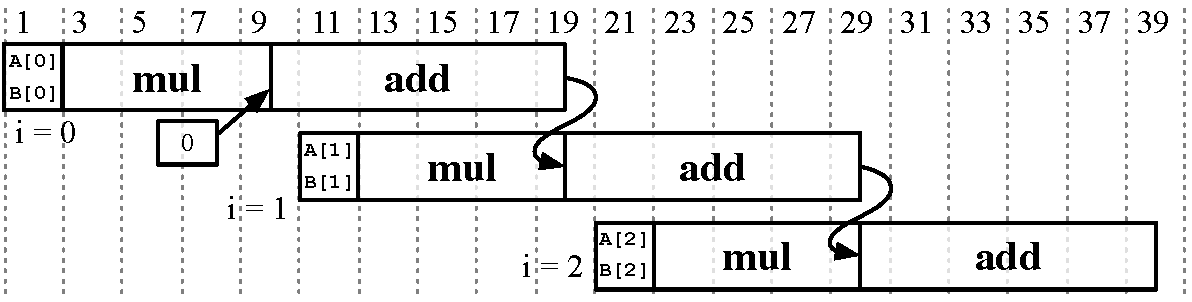
\includegraphics[width=0.8\linewidth]{sample_schedule_before}
    \caption{%
        The resulting schedule of the example program in generated.
    }\label{bg:fig:sample_schedule_before}
\end{figure}

Any valid schedule of this loop must satisfy the constraints imposed by
data-dependences.  For instance in our example, it is clear that in a
\emph{single} iteration, in the loop body, multiplication of \verb|A[i]|
and \verb|B[i]| must precede addition of \verb|d| and the multiplied
result.  Furthermore, in the $(i + 1)$-th iteration, access to the variable
\verb|d| must wait until \verb|d| is updated with a new value in the $i$-th
iteration, data-dependences therefore also exist on \verb|d| \emph{across}
loop iterations.  We call the former kind of dependences \emph{intra-iteration
dependences} and the latter \emph{inter-iteration dependences}.

Besides data-dependence constraints, the amount of resources available
also affects loop scheduling.  For instance, under our assumption in
Figure~\ref{bg:lst:dotprod} the RAM can only be read once per cycle, our
schedule thus should avoid reading from the same RAM in the same clock cycle.
We say a schedule is optimal, in the sense that the overall latency $L = (N -
1) \times \II + D$, is minimized, while none of the constraints are violated.
However with a much more complex program, finding the optimal schedule is
often an intractable task.  Limits on resource availability, along with
dependence constraints, make scheduling an NP-hard problem which is difficult
to solve optimally and efficiently~\cite{hwang91}.  In the following part
of this section, we discuss a heuristic technique known as \emph{modulo SDC
scheduling}~\cite{zhang13, canis14} used in LegUp to efficiently attack the
scheduling problem.


\subsection{Modulo SDC Scheduling}
\label{bg:sub:modulo_sdc_scheduling}

Many algorithms exist that can schedule loops efficiently.  For example,
Fan~\etal~\cite{fan08} proposed that a schedule can be found by formulating
the constraints into a satisfiability modulo theory (SMT) problem and use
an SMT solver to modulo schedule operations.  A technique, Iterative Modulo
Scheduling (IMS)~\cite{rau94}, has been a widely adopted by compilers that use
software pipelining to schedule instructions for Very Long Instruction Word
(VLIW) processors~\cite{mcnairy03}.  This method has also been widely adopted
in HLS tools such as PICO-NPA~\cite{schreiber02}, Trident~\cite{tripp05} and
LegUp~\cite{canis13, canis14}.  IMS for software pipelining~\cite{rau94},
however did not consider operator chaining, \ie~allowing operations
with combinational logics to be carried out in the same clock cycle.
Schreiber~\etal~\cite{schreiber02} in their adoption of IMS in HLS, found
operator chaining to be non-trivial in IMS and requires static timing analysis
of combinational components~\cite{canis14}.  A new method, the modulo SDC
scheduling algorithm, has recently gained traction and has been used by
Canis~\etal~\cite{canis14} in their LegUp and Zhang~\etal~\cite{zhang13},
because an SDC formulation is more suited to model the effect of chaining
operators, and therefore in this subsection an overview is provided for their
modulo SDC scheduling approach.

\subsubsection{Constructing the Data-Dependence Graph}

In the first stage of modulo SDC scheduling, dependence relations are extracted
from the body of this loop.  These dependence relations form a dependence
graph, where vertices are operations, and edges between pairs of vertices
indicate dependence relations.  This dependence graph can subsequently be used
to derive data-dependence constraints.  Figure~\ref{bg:fig:depgraph} shows
the complete dependence graph of the loop in our Figure~\ref{bg:lst:dotprod}
example.
\begin{figure}[ht]
    \centering
    \begin{tikzpicture}
        \node (ai)  at (0,0) {\texttt{A[i]}};
        \node (bi)  [right=of ai, xshift=5mm] {\texttt{B[i]}};
        \node (mul) [below right=of ai, xshift=-5mm, yshift=5mm]
            {$\times$};
        \node (sum) [left=of mul, xshift=-10mm] {\texttt{d}};
        \node (add) [below right=of sum, xshift=-4mm, yshift=5mm] {$+$};
        \draw[->] (ai)  -- node[auto]{\pair10} (mul);
        \draw[->] (bi)  -- node[auto]{\pair10} (mul);
        \draw[->] (mul) -- node[auto]{\pair70} (add);
        \draw[->] (sum) -- node[auto]{\pair00} (add);
        \draw[->,dashed]
            (add) to[out=-135, in=180] node[left=3pt]{\pair{10}{1}} (sum);
    \end{tikzpicture}
    \caption{%
        The dependence graph formed by the data-dependences in the loop body
        of the dot-product example in Figure~\ref{bg:lst:dotprod}.  The dashed
        edge highlights the inter-iteration dependence.
    }\label{bg:fig:depgraph}
\end{figure}

Intra-iteration dependence edges in the graph are each labelled with $\langle
l, 0 \rangle$, a 2-tuple attribute of integers accordingly.  The first integer
$l$ signifies the number of clock cycles that must elapse between the start of
the predecessor and the successor operations.  The latter value $0$ indicates
that the dependence occurs in the same iteration.  To illustrate, the edge
between the multiplier ``$\times$'' and adder ``$+$'' has an attribute $\langle
7, 0 \rangle$, because ``$\times$'' takes 7 cycles to generate an output.

Additionally, inter-iteration dependences create elementary cycles in the
dependence graph.  For example, in each iteration the initial value of \verb|d|
depends on the final value of \verb|d| from the previous iteration.  In this
graph we thus add an edge from the output of the addition to the variable
\verb|d|.  We further describe that this dependence has a \emph{dependence
distance} of $1$, as $1$ iteration must elapse between the start of each pair
of value updates and its corresponding use.  This edge is then further assigned
an attribute $\langle 10, 1 \rangle$ which signifies that the adder has a
latency of $10$ cycles, and this dependence has a distance $1$.

\subsubsection{Finding the Minimum Initiation Interval}

Modulo SDC scheduling owes its efficiency to assuming an initial constant
$\II$ and attempting to search for a schedule that satisfies all constraints.
This search stops if a feasible schedule is found, otherwise $\II$ can be
incremented by 1 and search again until we discover a valid schedule.  To
begin with, we can find a lower bound on $\II$---which we call the minimum
initiation interval $\MII$, such that all schedules with an $\II$ less than
$\MII$ violate some constraints---as our initial constant $\II$.  The $\MII$ is
determined by both the inter-iteration dependences and resource limits.  For
each of the both types of constraints, an $\MII$ can be found, respectively
known as recurrence-constrained $\MII$ ($\RecMII$) and resource-constrained
$\MII$ ($\ResMII$)~\cite{rau94, canis14, zhang13}.  We first introduce methods
to compute both values, then the overall $\MII$ can then be computed using the
following equation:
\begin{equation}
    \MII = \max\left(\RecMII, \ResMII\right).
\end{equation}

Firstly, we compute $\ResMII$, by finding the most constrained resources
in the loop, as these limits impact the $\ResMII$ value.  For example,
our example in Figure~\ref{bg:lst:dotprod} does not impose limits on the
number of floating-point operators that can be allocated, but assumes there
is a constraint which restricts the rate of memory accesses, \ie~only one
read is allowed in each clock cycle.  Because each iteration requires two
accesses to the same memory, a $\ResMII = 2$ will thus fully occupy the RAM
throughput.  To generalize this to all loops, we consider for each type of
operations $\mathrm{op}$ being used in the loop, the number of available
resources $r_\mathrm{op}$ for $\mathrm{op}$ and the number of occurrences
$n_\mathrm{op}(G)$ of $\mathrm{op}$ in the loop dependence graph $G$, to
evaluate $\left\lceil n_\mathrm{op}(G) / r_\mathrm{op} \right\rceil$, the
maximum ratio constitutes the final $\ResMII$, or equivalently:
\begin{equation}
    \ResMII = \max_{\mathrm{op}~\in~\mathrm{OpTypes}}
        \left\lceil
            \frac{n_\mathrm{op}(G)}{r_\mathrm{op}}
        \right\rceil,
\end{equation}
where $\mathrm{OpTypes}$ is a set of all types of operations, \eg~array
accesses, arithmetic units, and others.

The second step is to evaluate $\RecMII$ by ensuring for all cycles $c$ in the
graph $G$ the following inequalities hold:
\begin{equation}
    \forall c \in \mathrm{Cycles}(G):
        \sum_{e \in c} \mathrm{lat}(e) - \II \times
        \sum_{e \in c} \mathrm{dist}(e) \leq 0,
\end{equation}
where $\mathrm{Cycles}(G)$ computes the set of all cycles in the graph $G$;
$e \in c$ enumerates all edges in the cycle $c$; and for an edge $e$ between
two vertices $v_1$ and $v_2$ of the form $v_1 \xrightarrow{\langle l, d
\rangle} v_2$, $\mathrm{dist}(e)$ and $\mathrm{lat}(e)$ respectively evaluate
to the latency $l$ and dependence distance $d$.  Hence, $\sum_{e \in c}
\mathrm{lat}(e)$ and $\sum_{e \in c} \mathrm{dist}(e)$ respectively sum
the latencies and dependence distances along all edges in the cycle $c$.
Equivalently, we can derive an equation for $\RecMII$ for the graph $G$:
\begin{equation}
    \RecMII = \max_{c~\in~\mathrm{Cycles}(G)}
        \left\lceil \frac{%
            \sum_{e \in c} \mathrm{lat}(e)
        }{%
            \sum_{e \in c} \mathrm{dist}(e)
        }
        \right\rceil.
\end{equation}
For example, in the dependence graph (Figure~\ref{bg:fig:depgraph}) of our
simple program (Figure~\ref{bg:lst:dotprod}), one cycle,
\tikz[baseline=-0.65ex]{%
    \node(d) at (0, 0) {\texttt{d}};
    \node(plus) at (5ex, 0) {$+$};
    \draw[->] (d)-- (plus);
    \draw[->,dashed] (plus) to[out=115, in=65] (d);
},
exists and the sums of latencies and dependence distances along this cycle are
$10$ and $1$ respectively, thus the $\RecMII$ of this graph is $\lceil 10 / 1
\rceil = 10$.

The simplest possible method of finding $\RecMII$ is therefore to enumerate
all cycles in the graph and compute the ratio between sums of latencies and
dependence distances.  Unfortunately in the worst case, the number of cycles
is exponential to the number of edges in a graph, this approach could become
intractable for large loops.  An alternative method based on the Floyd-Warshall
shortest path algorithm which runs in polynomial time, is thus proposed
in~\cite{rau94} to efficiently find $\RecMII$.  This method will be further
discussed in Chapter~\ref{chp:latopt}, Section~\ref{lo:sub:latency_analysis}.

\subsubsection{Scheduling Operations}

After assuming a tentative constant $\II$, in module SDC scheduling, we try to
construct an SDC problem in order to solve for the schedule.  We aim to assign
each operation, corresponding to each vertex $v$ in the graph, to a time slot
$s_v$ when it begins its operation.  While in this process, the scheduling
must ensure that all assignments do not violate data-dependence and resource
constraints.  For instance if a multiply operation is allocated with a time
slot in the second clock cycle, in each iteration it will start computation in
the second clock cycle of that iteration.

To begin, we ignore the resource limits for now and formulate an SDC
problem for the dependence constraints.  For each dependence edge $u
\xrightarrow{\langle l, d \rangle} v$ from vertex $u$ to vertex $v$ in the
graph, it is possible to write down the following inequality, where $s_u$ and
$s_v$ are respectively the time slots for vertices $u$ and $v$:
\begin{equation}
    s_u - s_v \leq \II \times d - l.
\end{equation}
For instance, the edge $\times \xrightarrow{\langle 7, 0 \rangle} +$ is an
intra-iteration dependence, hence $\II$ does not constraint the scheduling
relation between these two operations and we substitute $d$ with $0$ and $l$
with $7$, and the $\II$ term vanishes, to derive~\eqref{bg:eq:sdc_intra} below,
whereas the back-edge $+ \xrightarrow{\langle 10, 1 \rangle} \mathtt{d}$
produces the following inequality in~\eqref{bg:eq:sdc_inter}:
\begin{align}
    s_\times - s_+ &\leq -7,
    \label{bg:eq:sdc_intra} \\
    s_+ - s_\mathtt{d} &\leq \II - 10.
    \label{bg:eq:sdc_inter}
\end{align}

Besides dependence constraints, additional constraints are used to limit the
length of critical paths in combinational logics, such that for instance, a
long chain of additions can be broken down into multiple cycles to guarantee
the frequency requirement.  For all paths $u \rightarrow \cdots \rightarrow
v$ between inter-iteration dependent vertices $u$ and $v$ consisting of
only combinational logics, it is possible to compute a critical path delay
$\mathrm{delay}(u, v)$.  This critical path delay is defined as the largest sum
of propagation delays of each intermediate operation along any combinational
path from $u$ to $v$.  For a pair of dependent vertices $u$ and $v$ such
that $\mathrm{delay}(u, v) > T_\mathrm{clk}$, where $T_\mathrm{clk} =
\frac{1}{f_\mathrm{clk}}$ and $f_\mathrm{clk}$ is the target clock frequency,
we can create the following constraint~\cite{cong06}:
\begin{equation}
    s_u - s_v \leq - \left\lceil
        \frac{
            \mathrm{delay}(u, v)
        }{
            T_\mathrm{clk}
        }
    \right\rceil + 1.
\end{equation}
This inequality ensures that for any the critical path delay between $u$
and $v$ greater than $T_\mathrm{clk}$, this path cannot be scheduled within
one clock cycle and it should be split into at least $ \left\lceil \frac{
\mathrm{delay}(u, v) }{ T_\mathrm{clk} } \right\rceil $ cycles.

Besides dependence and frequency constraints, Zhang~\etal~\cite{zhang13}
further introduces optional ones, such as lifetime constraints, which aim to
minimize the register requirements, and relative timing constraints, which can
be used to satisfy the timing requirement of user-specified I/O protocols.

The rationale of using the SDC formulation to model constraints is that
the feasibility of an SDC system and the corresponding solution, if it
exists, can be found efficiently.  More precisely, using the Bellman-Ford
algorithm~\cite{schrijver05}, it can run in $\Theta(l n)$ time, where
$l$ is the number of constraint inequalities and $n$ is the number of
variables~\cite{zhang13}.  Additionally, an SDC problem can be incrementally
solved, \ie~a new solution, if exists, can be updated in $O(m + n \log n)$
time when a constraint is added or removed, by using the algorithm presented
by Ramalingam~\etal~\cite{ramalingam99}.  In contrast, traditional ILP
scheduling techniques make use of $O(mn)$ variables to represent a scheduling
problem, where $m$ is the number of time slots and $n$ is the number of
operations~\cite{hwang91}, and solving this ILP problem often demands expensive
branch-and-bound procedures~\cite{zhang13} as ILP is NP-complete~\cite{karp10}.

Unfortunately, resources constraints, because of their non-linearity, cannot
be easily expressed as SDC constraints.  Therefore, a data structure called
\emph{modulo reservation table} (MRT) is used to keep track of resource
constraints as the loop is incrementally scheduled~\cite{canis14}.  The MRT
has $\II$ columns and each row tracks an available resource.  When a certain
resource is used in the time slot $s_u$, the MRT records an entry for this
resource in column $s_u \mod \II$ and the corresponding row of this resource.
To illustrate, consider our example in Figure~\ref{bg:lst:dotprod}, which
assumes a single read to the memory in one cycle for both arrays.  The MRT thus
has $\II = 10$ columns, and $1$ row for accessing the memory.  If \verb|A[i]|
is assigned with a time slot $0$, then a schedule assigning \verb|B[i]| to the
same time slot must be invalid, because a record exists for \verb|A[i]| in row
$1$ column $0$, and thus \verb|B[i]|, which is competing for the same resource,
hence must be scheduled in a later time slot.

A typical modulo SDC scheduling algorithm begins with a schedule without
resource constraints.  A priority function, is then used to sort all
resource-constrained operations by perturbation, which is to give greater
importance to operations that have a greater impact on the schedule when they
are moved~\cite{canis14}.  For each operator $u$ in this sorted list, if $u$ is
currently scheduled at time slot $t_u$ and does not have a resource conflict
in the MRT, a new constraint $s_u = t_u$ is constructed, otherwise a different
constraint $s_u \geq t_u + 1$ is used to ensure the operation $u$ is scheduled
one cycle later, so that it does not compete for the resource in time slot
$t_u$.  This newly created constraint is then tentatively added to the SDC
problem.  For a feasible resulting SDC problem, a new solution can be found
incrementally, otherwise the algorithm backtracks to a latest feasible SDC
formulation and try to schedule other operators before $u$.  A time budget can
also be used to limit the number of attempts to schedule resource-constrained
operators; if a valid schedule cannot be found under the given budget,
the $\II$ can be incrementing by $1$ to relax the dependence and resource
constraints, and the above mentioned procedure can be repeated until a valid
schedule is found.


\subsection{Obstacles in Adoption}
\label{sub:obstacles_in_adoption}

High-level synthesis, with its development-cost advantage over traditional RTL
design paradigm, is gaining traction in the circuit design community.  It is
however in its early phase, and these tools still pose challenges in terms of
using them as early adopters.

HLS tools may have limited support for HLL constructs.  For instance,
Vivado HLS requires pointer arrays to reference values or arrays of values,
platform-specific functions such as \verb|memcpy()| and \verb|memset()|
are supported but \verb|const| values must be used, and finally, while
tail-recursive functions written with C++ template constructs can be
transformed into loops in compile time, recursion in general cannot be
implemented~\cite{vivado_hls}.  Additionally, software programs often rely
on libraries, many of which are platform-specific, whereas in HLS\@, these
libraries may not be appropriate and may likely be unavailable.  These above
limitations make migrating existing software source code to a functional HLS
design a demanding task.

Optimizing C code for HLS could be a laborious process and requires expertise
in hardware design.  Although software compilers face similar challenges to
make programs run faster, experienced software programmers can often manually
fine-tune software implementations for performance, whereas currently only
engineers with an RTL-design background may be able to tailor source code
for the best circuit performance.  Winterstein~\etal~\cite{felix13} compared
manual RTL designs with HLS implementations of K-means clustering algorithms,
and discovered that with extensive manual code transformations, Vivado HLS can
still be persuaded to produce an efficient circuit.  When compared to the RTL
counterparts, their HLS designs achieved up to 40\% of the performance in terms
of area-time product.  Zhang~\etal~\cite{zhang15} implemented a convolutional
neural network (CNN) accelerator in Vivado HLS, they optimized their design by
program transformations techniques such as loop interchange, tiling, pipelining
and unrolling, and noticed that by enumerating combinations of loop tile sizes,
loop nest ordering and unroll factors, they were able to select the best
implementation by analytically estimating the throughput of each.  Similarly,
Suda~\etal~\cite{suda16} explored the design space of their CNN accelerator
by solving a resource-constrained throughput optimization problem, in order
to generate a high-performance CNN accelerator to be synthesized in Altera
OpenCL compiler~\cite{aoc}.  HLS tools can provide some syntactic constructs
to automate lower-level code transformations such as instruction parallelism,
loop pipelining and unrolling.  It is however up to the engineer to decide
how to utilize these transformations, and laboriously determine if they will
improve their design.  Higher-level optimizations such as the manual design
space exploration explained in earlier examples, if automated, may allow tools
to vastly improve the performance of HLS applications.  Making use of these
techniques in HLS, however, remains a significant challenge.

HLS tools can often make use techniques such as loop pipelining discussed in
Section~\ref{bg:sub:modulo_sdc_scheduling} to detect and exploit parallelism at
the instruction-level.  Coarser-grain parallelism, which is tightly associated
with the algorithmic details, is however much more complex~\cite{nane15},
and many optimization opportunities are not yet exploited by HLS tools.  For
instance, unlike the CPU, which has a monolithic storage and thus their
performance is often limited by the memory wall, the FPGA has dedicated RAM
blocks in the logic fabric to distribute memory bandwidth via data reuse.  HLLs
such as C were designed with a mindset of the von Neumann architecture, and the
source code in C typically do not specify how the memory hardware is utilized.
For this reason, HLS tools must be able to intelligently partition a monolithic
memory into smaller chunks that can be accessed in parallel, in order to
maximize performance; how to attain this is still a challenging research
area~\cite{cong11, cong12, wang13, felix15}.

Circuits produced by HLS tools are expected to be semantic-preserving.  It
means that they should be functional equivalent to the original C programs; in
other words, for any given program inputs, the tools should guarantee that the
computed outputs from the original C code and the synthesized circuit should
be identical.  A different class of optimizations, which we call \emph{lossy
optimization}, break this promise by optimizing data-paths in a way that may
impact numerical accuracy.  HLS tools could benefit from these optimizations
in the future, which bring further performance improvements that can not
be attained by traditional optimizations alone.  Because these approaches
could affect numerical accuracy, performance optimization and round-off error
analysis may be carried out simultaneously.  We will further discuss lossy
optimization methods such as expression balancing employed by Vivado HLS and
LegUp in Section~\ref{bg:sec:discovering_equivalent_programs} and word-length
optimization in Section~\ref{bg:sec:wordlength}.

\section{Abstract Interpretation}
\label{bg:sec:abstract_interpretation}

This section starts by introducing the basic concepts of program semantics
and the abstract interpretation framework, a static analysis technique.  This
is then extended to define a scalable analysis capturing accuracy.  Later in
Chapter~\ref{chp:progopt} we accommodate sequential statements, \iflit~branches
and \whilelit~loops in the accuracy analysis, and in Chapter~\ref{chp:latopt},
we further improve our analysis by supporting multi-dimensional arrays.


\subsection{Intervals}
\label{bg:sub:intervals}

We illustrate these concepts by putting the familiar idea of \emph{interval
arithmetic}~\cite{moore} in the framework of abstract interpretation. As
an illustration, consider the following expression and its DFG in
Figure~\ref{bg:fig:sample_tree}\@:
\begin{equation}
    (a + b) \times (a + b)
    \label{bg:eq:absint_sample}
\end{equation}
\begin{figure}[ht]
    \centering
    \includegraphics[scale=0.6]{sample_tree}
    \caption{The DFG for the sample expression.}\label{bg:fig:sample_tree}
\end{figure}

We may wish to ask: if initially $a$ and $b$ are real numbers in the range of
$[0.2, 0.3]$ and $[2, 3]$ respectively, what would be the outcome of evaluating
this expression with real arithmetic? A straightforward approach is simulation.
Evaluating the expression for a large quantity of inputs will produce a set
of possible outputs of the expression. However the simulation approach is
unsafe, since there are infinite number of real-valued inputs possible and it
is infeasible to simulate for all.

A better method might be to represent the possible values of $a$ and $b$ using
ranges. To compute the ranges of its output values, we could operate on ranges
rather than values (note that the superscript $\sharp$ denotes ranges). Assume
that $a^\sharp_{init} = [0.2, 0.3]$, $b^\sharp_{init} = [2, 3]$, which are the
input ranges of $a$ and $b$, and $\enter{l}$ where $l \in \{1, 2, 3, 4\}$ are
the intervals of the outputs of the boxes labelled with $l$ in the DFG\@. We
extract the data flow from the DFG to produce the following set of equations:
\begin{equation}
    \begin{aligned}
        \enter{1} &= a^\sharp_{init} \\
        \enter{2} &= b^\sharp_{init} \\
        \enter{3} &= \enter{1} + \enter{2} \\
        \enter{4} &= \enter{3} \times \enter{3}
    \end{aligned}
    \label{bg:eq:absint_sample_analysis}
\end{equation}
For the equations above to make sense, addition and multiplication need to be
defined on intervals. We may define the following interval operations:
\begin{equation}
    \begin{aligned}
        \interval{a}{b} + \interval{c}{d} &= \interval{a + c}{b + d} \\
        \interval{a}{b} - \interval{c}{d} &=  \interval{a - d}{b - c} \\
        \interval{a}{b} \times \interval{c}{d} &=
            \interval{\min(s)}{\max(s)} \\
        \text{where~} s &= \{ a \times c, a \times d, b \times c, b \times d \}
    \end{aligned}
    \label{bg:eq:interval_operations}
\end{equation}
The solution to the set of~\eqref{bg:eq:absint_sample_analysis} for $\enter{4}$
is $[4.84, 10.89]$, which represents a safe bound on the output at the end
of program execution. Note that in actual execution of the program, the
semantics represent the values of intermediate variables, which are real
values. In our case, a set of real values forms the set of all possible
values produced by our code. However computing this set precisely is not,
in general, a possible task. Instead, we use abstract interpretation based
on intervals, which gives the abstract semantics of this program. Here, we
have achieved a classical interval analysis by \emph{defining} the meaning of
addition and multiplication on abstract mathematical structures (in this case
intervals) which capture a safe approximation of the original semantics of the
program.

Later in Sections~\ref{so:sec:resource}~and~\ref{so:sec:equivalent} of
Chapter~\ref{chp:stropt}, we further generalize the idea by defining the
meaning of these operations on more complex abstract structures which allow
us to scalably reason about the area of FPGA implementations and equivalent
program structures respectively.


\subsection{Accuracy Analysis}
\label{bg:sub:accuracy}

Because we optimize numerical programs in a way that may have significant
impact on accuracy, and one of our objectives is to minimize round-off error
in the process, it is necessary to perform accuracy analysis on optimized
candidates.

Since our numerical programs make use of floating-point arithmetic, we first
introduce the concepts of the floating-point representation~\cite{ieee754}. Any
values $v$ representable in floating-point with standard exponent offset can be
expressed with the format given by the following equation:
\begin{equation}
    v = s \times 2^{e + 2^{k - 1} - 1} \times 1.{m_1 m_2 m_3 \ldots m_p}
    \label{bg:eq:floating_point}
\end{equation}
In~\eqref{bg:eq:floating_point}, the bit $s$ is the sign bit, the $k$-bit
unsigned integer $e$ is known as the exponent bits, and the $p$-bits $m_1 m_2
m_3 \ldots m_p$ are the mantissa bits, here we use $1.{m_1 m_2 m_3 \ldots m_p}$
to indicate a fixed-point number represented in unsigned binary format.

Because of the finite characteristic of IEEE 754 floating-point format, it
is not always possible to represent exact values with it. Computations in
floating-point arithmetic often induces roundoff errors. Therefore, following
Martel~\cite{martel07}, we bound with ranges the values of floating-point
calculations, as well as their roundoff errors. Our accuracy analysis
determines the bounds of all possible outputs and their associated range of
roundoff errors for expressions. For example, assume that real variables $a
\in [0.2, 0.3]$, $b \in [2.3, 2.4]$, it is possible to derive that in single
precision floating-point computation with rounding to the nearest, ${(a + b)}^2
\in [6.24999857, 7.29000187]$ and the error caused by this computation is
bounded by $[-1.60634534\times10^{-6}, 1.60634534\times10^{-6}]$.

We employ abstract error semantics for the calculation of errors described
in~\cite{ioualalen, martel07}. First we define the domain $\errorset
= \floatintervalset\times\intervalset$, where $\intervalset$ and
$\floatintervalset$ respectively represent the set of real intervals, and
the set of floating-point intervals (intervals exactly representable in
floating-point arithmetic). The value $(x^\sharp, \mu^\sharp) \in \errorset$
represents a safe bound on floating-point values and the accumulated error
represented as a range of real values. Then addition and multiplication can be
defined for the semantics as in~\eqref{bg:eq:error_semantics}:
\begin{equation}
    \begin{aligned}
        \left( x^\sharp_1, \mu^\sharp_1 \right) +
        \left( x^\sharp_2, \mu^\sharp_2 \right)
    &=  \left(
            \roundup{x^\sharp_1 + x^\sharp_2},
            \mu^\sharp_1 + \mu^\sharp_2 +
            \rounddown{x^\sharp_1 + x^\sharp_2}
        \right) \\
        \left( x^\sharp_1, \mu^\sharp_1 \right) -
        \left( x^\sharp_2, \mu^\sharp_2 \right)
    &=  \left(
            \roundup{x^\sharp_1 - x^\sharp_2},
            \mu^\sharp_1 - \mu^\sharp_2 +
            \rounddown{x^\sharp_1 - x^\sharp_2}
        \right) \\
        \left( x^\sharp_1, \mu^\sharp_1 \right) \times
        \left( x^\sharp_2, \mu^\sharp_2 \right)
    &=  \left(
            \roundup{x^\sharp_1 \times x^\sharp_2},
            x^\sharp_1 \times \mu^\sharp_2 + x^\sharp_2 \times \mu^\sharp_1 +
            \mu^\sharp_1 \times \mu^\sharp_2 +
            \rounddown{x^\sharp_1 \times x^\sharp_2}
        \right) \\
    &\qquad\qquad\qquad\qquad\qquad\qquad\text{~for~}
        \left( x^\sharp_1, \mu^\sharp_1 \right) \in \errorset,
        \left( x^\sharp_2, \mu^\sharp_2 \right) \in \errorset
    \end{aligned}
    \label{bg:eq:error_semantics}
\end{equation}

The addition, subtraction and multiplication of intervals follow
the standard rules of interval arithmetic defined earlier
in~\eqref{bg:eq:interval_operations}.  In~\eqref{bg:eq:error_semantics}, the
function $\rounddownop: \intervalset \to \intervalset$ determines the range
of roundoff error due to the floating-point computation under one of the
\emph{rounding modes} $\circ \in \{ -\infty, \infty, 0, \neg0, \sim \}$ which
are round towards negative infinity, towards infinity, towards zero, away from
zero and towards nearest floating-point value respectively. It is defined as:
\begin{equation}
    \begin{aligned}
        & \downarrow^\sharp_\circ([a, b]) = \left\{
            \begin{aligned}
                & \left[ -\frac{z}{2}, \frac{z}{2}\right]
                    & \quad \circ & \text{~is~}\sim \\
                & \left[ -z, z\right]
                    & \quad \circ & \in \{ -\infty, \infty, 0, \neg0 \}
            \end{aligned}
        \right. \\
        & \qquad\qquad\qquad\qquad \text{where~} z = \max(ulp(a), ulp(b))
    \end{aligned}
\end{equation}
Here $z$ denotes the maximum rounding error that can occur for values
within the range $[a, b]$, and the unit of the last place (ulp) function
$ulp(x)$~\cite{muller} characterizes the distance between two adjacent
floating-point values $f_1$ and $f_2$ satisfying $f_1 \leq x \leq
f_2$~\cite{goldberg}. In our analysis, the function $ulp$ is defined as:
\begin{equation}
    ulp(x) = 2^{e(x) + 2^{k - 1} - 1} \times 2^{-p}
\end{equation}
where $e(x)$ is the exponent of $x$, $k$ and $p$ are the parameters of the
floating-point format as defined in~\eqref{bg:eq:floating_point}. The function
$\roundupop: \intervalset \to \floatintervalset$ computes the floating-point
bound from a real bound, by rounding the infimum $a$ and supremum $b$ of the
input interval $[a, b]$:
\begin{equation}
    \roundupop\left(\left[a, b\right]\right)
    = {\left[
        \uparrow_\circ{\left(a\right)},
        \uparrow_\circ{\left(b\right)}
    \right]}_\floatset
\end{equation}
where the subscript $\floatset$ indicates the interval is a floating-point
interval, and we define $\uparrow_\circ: \realset \to \floatset$ to be the
function that rounds a real number to a floating-point value, under the
rounding mode $\circ$.

Expressions can be evaluated for their accuracy by the method as follows.
Initially the expression is parsed into a data flow graph (DFG). By way of
illustration, the sample expression ${(a + b)}^2$ has the tree structure
in Figure~\ref{bg:fig:sample_tree}. Then the exact ranges of values of $a$ and
$b$ are converted into the abstract semantics using a cast operation as in
\eqref{bg:eq:cast}:
\begin{equation}
    \mathrm{cast}\left(x^\sharp\right) = \left(
        \roundup{x^\sharp}, \rounddown{x^\sharp}
    \right)
    \label{bg:eq:cast}
\end{equation}
For example, for the real variable $a \in [0.2, 0.3]$ under single precision
with rounding to nearest,
\begin{equation}
    \mathrm{cast}\left([0.2, 0.3]\right) = \left(
        {\left[0.200000003, 0.300000012\right]}_\floatset,
        \left[-1/67108864, 1/67108864\right]
    \right)
\end{equation}
After this, the propagation of bounds in the data flow graph is carried out as
described in Section~\ref{bg:sub:intervals}, where the difference is the abstract
error semantics defined in~\eqref{bg:eq:error_semantics} is used in lieu of the
interval semantics. At the root of the tree (\ie~the exit of the DFG) we find
the value of the accuracy analysis result for the expression.

\section{Intermediate Representations}
\label{bg:sec:intermediate}

Intermediate representations (IRs) are data structures designed to be
independent of the machine architecture and source language.  They are often
invented with the intention to ease program analysis and optimization in mind,
by abstracting information from the original program that are irrelevant to our
objectives.  In this section, we introduce several categories of existing IRs,
and delve deeper into the advantages and disadvantages of each.

\subsection{Static Single Assignment Form and Control-Flow Graph}
\label{bg:sub:ssa_cfg}

Traditionally, \emph{static single assignment} (SSA) form~\cite{alpern88,
rau92} together with \emph{control-flow graph} (CFG) are used to represent
data- and control-flow of a program~\cite{cytron91}, because they are more
favorable program representations on which optimization passes can be
implemented, when compared to the original HLL or the output language.  SSA can
be advantageous in implementing conventional optimization techniques, \eg~code
motion~\cite{cytron86}, removing redundant computations~\cite{rosen88},
and constant propagation~\cite{cytron91}.  Because the LLVM intermediate
representation (LLVM IR)~\cite{llvm_ir} is based on SSA and CFG, and is
commonly used in many HLS tools such as LegUp~\cite{legup}, we introduce SSA
and CFG by compiling the dot-product example in Figure~\ref{bg:lst:dotprod}
into as shown in Figure~\ref{bg:lst:dotprod_ll}.
\begin{figure}[ht]
    \centering
    \begin{lstlisting}[language=LLVM]
define float @dotprod(
    float* nocapture readonly %A,
    float* nocapture readonly %B) #0
{
; <label>:0
  br label %2

; <label>:1         ; preds = %2
  ret float %8

; <label>:2         ; preds = %2, %0
  %i.02 = phi i32 [ 0, %0 ], [ %9, %2 ]
  %d.01 = phi float [ 0.000000e+00, %0 ], [ %8, %2 ]
  %3 = getelementptr inbounds float, float* %A, i32 %i.02
  %4 = load float, float* %3, align 4, !tbaa !2
  %5 = getelementptr inbounds float, float* %B, i32 %i.02
  %6 = load float, float* %5, align 4, !tbaa !2
  %7 = fmul float %4, %6
  %8 = fadd float %d.01, %7
  %9 = add nuw nsw i32 %i.02, 1
  %exitcond = icmp eq i32 %9, 1024
  br i1 %exitcond, label %1, label %2
}
    \end{lstlisting}
    \caption{%
        The compiled and optimized LLVM IR output from the dot-product example
        in Figure~\ref{bg:lst:dotprod}.
    }\label{bg:lst:dotprod_ll}
\end{figure}

The LLVM IR of our example function consists of parts that are known as
\emph{basic blocks} (BB), each BB in turn often contains a label that
uniquely identifies the BB, a list of LLVM IR statements in SSA form
without any branches, \ie~the statements are executed sequentially, and a
terminator instruction, which is typically a branch instruction that leads
the control-flow to a different BB, by referencing a BB label, or a function
return.

The LLVM framework implicitly constructs a CFG from the IR code, which is a
directed graph representing the control-flow of a program.  The vertices in
the CFG constitute BBs, while the edges indicate the control-flow directions
(\ie~branches to other BBs), often with predicate attributes to determine
whether the branch is taken.  For instance, we consider the first line of third
BB in Figure~\ref{bg:lst:dotprod_ll}:
\begin{lstlisting}[language=LLVM, basicstyle=\tt]
    ; <label>:2     ; preds = %2 %0
\end{lstlisting}\vspace{-16.5pt}
which indicates it has a label value $2$ and the control-flow coming to this
BB is from either BB2 or BB0, here we use BB$n$ as a shorthand denoting a
BB labelled $n$.  Additionally, this BB ends with the branch terminator
instruction:
\begin{lstlisting}[language=LLVM, basicstyle=\tt]
    br i1 %exitcond, label %1, label %2
\end{lstlisting}\vspace{-16.5pt}
This instruction directs the control-flow to BB1 or BB2, and the variable
\verb|%exitcond| in the terminator instruction decides which branch is taken.
Finally, the complete CFG is shown in Figure~\ref{bg:fig:dotprod_cfg}.  It is
noteworthy that BB2 has two edges that leads to either \verb|BB1| or \verb|BB2|
itself.  If \verb|%exitcond| evaluates to false (\textbf{ff}), then another
iteration of BB2 will commence, otherwise (\textbf{tt}) the exit condition is
satisfied and will lead the control-flow to \verb|BB1|.
\begin{figure}[ht]
    \centering
    \tikzstyle{block} = [
        draw, fill=white, rectangle, minimum height=2em, minimum width=3em
    ]
    \tikzstyle{tmp} = [coordinate]
    \begin{tikzpicture}
        \node [] (entry) {Entry};
        \node [block, below of=entry, node distance=4em] (bb0) {\texttt{BB0}};
        \node [block, below of=bb0, node distance=4em] (bb1) {\texttt{BB1}};
        \node [block, below of=bb1, node distance=4em] (bb2) {\texttt{BB2}};
        \node [tmp, right of=bb1, node distance=5em] (bb1tr) {};
        \node [tmp, left of=bb2, node distance=8em] (bb2tl) {};
        \node [tmp, right of=bb2, node distance=8em] (bb2tr) {};
        \node [below of=bb2, node distance=4em] (exit) {Exit};
        \draw [->] (entry) -- (bb0);
        \draw [- ] (bb0)    to[out=0, in=90]    (bb1tr);
        \draw [->] (bb1tr)  to[out=-90, in=0]   (bb2);
        \draw [- ] (bb1)    to[out=180, in=90]  (bb2tl);
        \draw [->] (bb2tl)  to[out=-90, in=180] (exit);
        \draw [->] (bb2) -- node[auto, swap]{\textbf{tt}} (bb1);
        \draw [->] (bb2) to[out=-150, in=150, loop]
            node[auto, swap]{\textbf{ff}} (bb2);
    \end{tikzpicture}
    \caption{The CFG of the LLVM IR code in Figure~\ref{bg:lst:dotprod_ll}.
    }\label{bg:fig:dotprod_cfg}
\end{figure}

Each BB contains sequential computations that are represented by SSA
instructions.  The SSA form describes the operations in the original
program, such that each variable in it is assigned exactly one value.

The sequence of instructions that assigns to \verb|%3|-\verb|%9| in
Figure~\ref{bg:lst:dotprod_ll} carries out most of the computations in the
program.  It starts by reading \verb|A[i]| and \verb|B[i]|, multiplying them
together, then add the result with \verb|d| to form a new variable, and
finally, the iteration value is accumulated by $1$.  It may seem unusual that
both the accumulated sum of products and the iteration value are not assigned
to \verb|d| and \verb|i| respectively.  We can imagine two BBs, one initializes
\verb|d| and \verb|i| to zeros, the other accumulates these two variables in
a loop.  As all variables must be assigned once only, one of the BBs should
use different names for these two variables.  When the control-flow of these
two BBs join, we must introduce a way to read from the variables that are
assigned in the two BBs in the succeeding BB\@.  A new instruction, called the
$\phi$-function is therefore defined for our purpose.  The $\phi$-function
accepts two variable names as its inputs, and produce the value of either
variable as its output, determined by which preceding BB the control-flow came
from.  For example, in LLVM IR, the instruction:
\begin{lstlisting}[language=LLVM, basicstyle=\tt]
    %d.01 = phi float [ 0.000000e+00, %0 ], [ %8, %2 ]
\end{lstlisting}\vspace{-16.5pt}
shows that if the control-flow originated from BB0, then a constant zero is
returned, otherwise the control-flow had to come from BB2 and the value of
\verb|%8| is used instead.

The rationale of SSA is that we can abstract away anti- and output dependences
by never assigning to the same variable twice, while only true data-flow
dependences remain.  Anti-dependence is a dependence relation when a read
operation must precede a write to the same variable, and output dependence is
when two writes refer to the same location.  By removing these dependences
and deferring the analysis of them, certain program optimization analyses
can run much more efficiently.  Analyses that may benefit from this include
scheduling~\cite{rau94}, and liveness analysis (figure out the life time
of variables to reduce register requirements)~\cite{cytron91}, detecting
opportunities of parallelism~\cite{cytron87}, and finding equivalent parts in
the program~\cite{alpern88}.

In a cyclic CFG, the control-flow could potentially revisit a BB, and
instructions in this BB will inevitably assign a different value to the
same variable, which forms anti- and output dependences, which could have a
detrimental effect on efficient loop pipelining in some computing machines.  An
alternative IR, the \emph{dynamic single assignment} (DSA) form~\cite{rau92}
can therefore be used in place of the SSA to address this issue.  The DSA
defines a linear sequence of virtual registers for each variable, such that
every time the variable is assigned in a dynamic execution path, a new virtual
register is used.

\subsubsection{Alternatives to SSA and CFG}

There are a number of alternative IRs that are similar in construction to
the SSA and CFG approach in LLVM IR\@.  For instance, the data-dependence
graph~\cite{rau94} introduced in Section~\ref{bg:sub:sdc} are designed
for the purpose of capturing data-flow dependences in polyhedral methods.
\emph{Data-flow graph} (DFG) is a popular alternative to SSA, which is often
a directed acyclic graph (DAG) that do not contain cyclic paths.  In general,
a DFG's vertices are input, output and operation nodes, and the edges capture
the dependences between these nodes.  Both of them, however, generally do
not preserve enough information for us to reconstruct a program from the
graph itself.  A group of data structures, known as \emph{control/data flow
graphs} (CDFGs)~\cite{orailoglu86}, is commonly used to represent programs in
HLS tools, \eg~SPARK~\cite{gupta04}.  A CDFG resembles a CFG such as the one
used in LLVM IR, but in lieu of using sequential instructions in SSA form in
graph vertices, each vertex contains a \emph{data-flow graph} (DFG), where no
SSA temporary variables are used and data-flow dependences can by explicitly
identified by edges.


\subsection{Equality Saturation}
\label{bg:sub:equality_saturation}

The IRs we discussed above are all used to analyze and transform the underlying
program structure, so as to produce a new representation of the optimized
program.  In a conventional optimizing compiler, program optimization is
often carried out in a sequence of transformation passes, where each pass
accepts a program, often written in a certain IR, and produces an optimized
program in the IR\@.  The traditional practice is to always apply these
optimization phases in a fixed order, but a good ordering of these phases
is crucial to achieve a good optimized result, and the optimal ordering
varies across applications being compiled~\cite{almagor04}.  The process of
finding the optimal ordering is known as the \emph{phase-ordering problem},
which is in general undecidable~\cite{touati06} and hence is a difficult
problem.  Moreover, programs running CPUs or GPUs usually care only about
their throughput, in contrast, designs on FPGAs concern us with additional
objectives besides run time, such as power consumption and resource utilization
that impact the quality of synthesized circuit.  Multiple designs that
trade-off these objectives could exist, and which design to choose relies
on the specifics of the use case.  It is therefore sensible to explore the
design space by optimizing multiple objectives simultaneously.  For the
above reasons, it is desirable to have an IR and the associated optimization
procedures to efficiently discover equivalent structures that lead to different
implementations of the original program.

In software, a novel approach called \emph{equality saturation} is proposed
in~\cite{tate09} to find multiple possible optimized variants of the original
program, and subsequently deal with the phase-ordering problem.  It creates
a new graph-based IR, \emph{program expression graph} (PEG), to encode the
effects of executing the program.

To begin, we review the structure of the PEG, by considering a simple loop
example in Figure~\ref{bg:fig:factorial}.  By understanding how the PEG can
be evaluated for the output values, we can interpret how the PEG captures the
control- and data-flow information of the program.  PEGs, similar to arithmetic
expressions expressed in a tree structure, can be evaluated in a bottom-up
fashion, by recursively propagating computed values from the leave nodes to the
root of the tree.  However, unlike arithmetic expressions which are acyclic,
edges in PEGs may form cycles to express loops in the original program.
\begin{figure}[ht]
    \newsavebox{\factlstbox}
    \begin{lrbox}{\factlstbox}
    \begin{lstlisting}
int x = 1;
int y = 1;
while (y <= 10)
{
    x = y * x;
    y = y + 1;
}
    \end{lstlisting}
    \end{lrbox}
    \centering
    \subfloat[The original program.]{%
        \begin{minipage}{0.4\textwidth}
            \usebox{\factlstbox}
        \end{minipage}\label{bg:lst:factorial_c}
    }
    \subfloat[The resulting PEG.]{%
        \begin{minipage}{0.5\textwidth}
            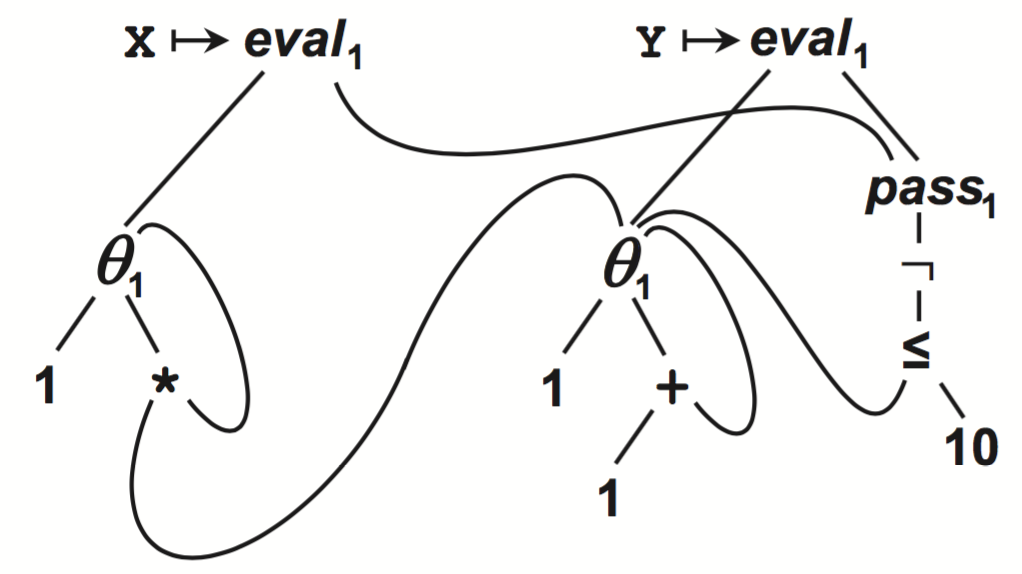
\includegraphics[width=\textwidth]{bg/fig/factorial_peg.png}
        \end{minipage}\label{bg:fig:factorial_peg}
    }
    \caption{%
        A simple loop which computes the factorial of 10, and the resulting
        PEG\@.  This example and its PEG, showing computations that lead to the
        final \texttt{x} and \texttt{y}, is taken from~\cite{tate09}.
    }\label{bg:fig:factorial}
\end{figure}

\subsubsection{Data-Flow Nodes}

All loops in the PEG are formed by $\theta$ nodes, which is used in the
following form:
\begin{center}
    \vspace{-16.5pt}
    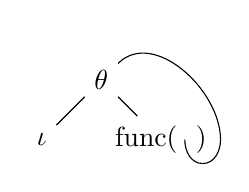
\begin{tikzpicture}
        \node (theta) at (0, 0) {$\theta$};
        \node (init) at (-5ex, -5ex) {$\iota$};
        \node (func) at (5ex, -5ex) {$\mathrm{func}(~~)$};
        \node[coordinate] (input) at (7ex, -5ex) {};
        \node[coordinate] (mid1) at (8.5ex, -7ex) {};
        \node[coordinate] (mid2) at (10ex, -5ex) {};
        \draw[-] (theta) -- (init);
        \draw[-] (theta) -- (func);
        \draw[-] (input) to[out=-90, in=180] (mid1);
        \draw[-] (mid1) to[out=0, in=-90] (mid2);
        \draw[-] (mid2) to[out=90, in=45] (theta);
    \end{tikzpicture}
    \vspace{-16.5pt}
\end{center}
where it accepts two child graphs, $\iota$ and $\mathrm{func}$, and
$\mathrm{func}$ further takes the $\theta$ node as one of its inputs to
form a complete cycle.  Evaluating a $\theta$ node produces a list of
values computed iteratively by the node's subgraph.  The first value in the
list, is the computed result of $\iota$, which we name $i$, and values in
the rest of the sequence are iteratively computed by $\mathrm{func}$.  In
functional programming, this is similar to iteratively computing the fixpoint
$\fixpoint{F}$ of an initial list $[i]$, which is defined as:
\begin{equation}
    \fixpoint{F} ([i]) = \lim_{n \to \infty} F^n ([i]),
    \quad\text{where~}
    F(v) = \mathrm{prepend}\left(
        \iota, \mathrm{map}\left( \mathrm{func}, v \right)
    \right)
\end{equation}
here, $\mathrm{map}(\mathrm{func}, v)$ applies the subgraph computation
$\mathrm{func}$ to all elements in the list $v$, and $\mathrm{prepend}(\iota,
v^\prime)$ prepends the element $\iota$ to the list $v^\prime$.

For example, the following subgraph in Figure~\ref{bg:fig:factorial_peg}
evaluates to the sequence $[1, 2, 3, 4, \mathellipsis]$:
\begin{center}
    \vspace{-16.5pt}
    \begin{tikzpicture}
        \node (theta) at (0, 0) {$\theta_1$};
        \node (init) at (-5ex, -5ex) {$1$};
        \node (add) at (5ex, -5ex) {$+$};
        \node (one) at (0, -10ex) {$1$};
        \node[coordinate] (mid) at (8ex, -5ex) {};
        \draw[-] (theta) -- (init);
        \draw[-] (theta) -- (add);
        \draw[-] (add) -- (one);
        \draw[-] (add) to[out=-45, in=-90] (mid);
        \draw[-] (mid) to[out=90, in=45] (theta);
    \end{tikzpicture}
    \vspace{-16.5pt}
\end{center}

It is noteworthy that $\theta$ nodes may have subscripts.  For instance,
in Figure~\ref{bg:fig:factorial_peg}, both nodes $\theta_1$ share the same
subscript $1$.  This is used to indicate that the two sequences produced
by both $\theta$ nodes iterate simultaneously, \ie~they share the same
iteration count so that a new value for \verb|x| can be computed as we update
\verb|y|.  Therefore, the $\theta_1$ node in the left of this figure produces
a sequence of the factorials of $[1, 2, 3, \mathellipsis]$, \ie~$[1, 2, 6, 24,
\mathellipsis]$.

Computation nodes, such as arithmetic $+$ and boolean operators $\leq$ and
$\neg$ in Figure~\ref{bg:fig:factorial_peg}, operates on a list of values, by
performing the computation on each value in the list.

For instance, the $\leq$ node accepts two inputs, the sequence $[1, 2, 3,
\mathellipsis]$ derived earlier, and a scalar $10$, computes the result of $x
\leq 10$ for each element $x$ in the sequence, and finally produces the list,
where $\truelit$ and $\falselit$ respectively denote true and false boolean
values:
\begin{equation}
    [
        \truelit, \truelit, \truelit, \truelit, \truelit,
        \truelit, \truelit, \truelit, \truelit, \truelit,
        \falselit, \falselit, \falselit, \mathellipsis
    ].
\end{equation}
The subsequent $\neg$ node then negates all elements in the list:
\begin{equation}
    [
        \falselit, \falselit, \falselit, \falselit, \falselit,
        \falselit, \falselit, \falselit, \falselit, \falselit,
        \truelit, \truelit, \truelit, \mathellipsis
    ].
    \label{bg:eq:bool_seq}
\end{equation}

\subsubsection{Control-Flow Nodes}

The $\theta$ node encodes an infinite sequence of computed values, whereas
the output value of the program is a scalar.  By further representing
control-flow information in PEG, it becomes possible to refer to a
single value in this sequence, as the output of the program.  To do so,
Tate~\etal~\cite{tate09} further introduce $\mathrm{pass}$ and $\mathrm{eval}$
nodes.  The $\mathrm{pass}$ node finds the first true ($\truelit$) value
in a sequence of boolean values, and returns the index of this value, and
$\mathrm{eval}$ takes two child nodes, where the first node evaluates to a list
$v$ of values, and the second is an scalar $n$ used to select a scalar value
from $l$, as the output of this node.

To illustrate, the $\mathrm{pass}_1$ node finds the first $\truelit$ in the
list~\eqref{bg:eq:bool_seq}, $11$.  The $\mathrm{eval}$ node of the output
variable \verb|y| subsequently fetches the $11$-th item from the list $[1, 2,
3, 4, \mathellipsis]$ we produced earlier, which is $11$.  Similarly we can
apply the same process to find that the output \verb|x| is $10!\,$, \ie~the
factorial of 10.

By using $\mathrm{pass}$ and $\mathrm{eval}$ nodes to represent the
control-flow in an algebraic fashion, and mixing data- and control-flows
together in the graphical representation, PEGs provide us with greater
opportunities to optimize data-flow across control-flow boundaries and vice
versa.  Simple equivalence rules can be defined for these nodes algebraically.
For instance, arithmetic operators can be distributed over $\theta$ and
$\mathrm{eval}$, \eg~$\mathrm{eval}(j, k) + i \equiv \mathrm{eval}(j + i, k)$.
Complex transformations can therefore be deductively constructed from these
simple equivalence rules.

\subsubsection{Equivalence Finding}

By applying transformation passes to the PEG, their approach detects the
incremental modifications, and append these changes to the original PEG\@.  The
new changes, represented as extra structures in the PEG, are linked to their
corresponding equivalent nodes by equivalence edges.  These edges indicate a
pair of subgraphs are equivalent, forming a PEG with equivalent structures,
or named E-PEG, that could capture multiple PEGs in the same structure.  The
resulting E-PEG is similar to the one in Figure~\ref{bg:fig:epeg}, where dashed
edges indicate equivalences.  It is notable that each edge allows a binary
choice, therefore the number of PEGs can be represented in an E-PEG could be
exponential in the number of equivalence edges.
\begin{figure}[ht]
    \centering
    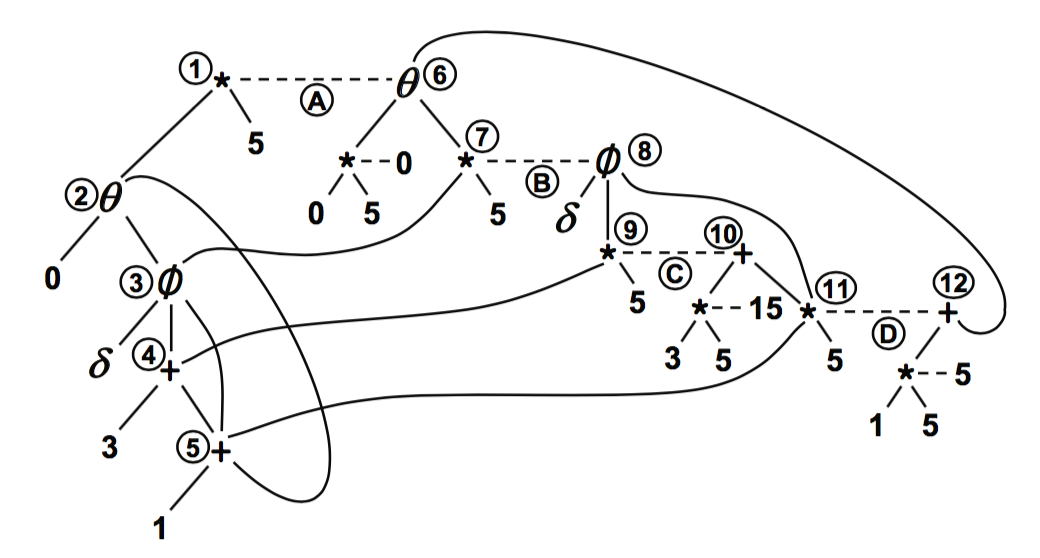
\includegraphics[width=0.8\linewidth]{bg/fig/epeg.png}
    \caption{An simple E-PEG example, taken from~\cite{tate09}.
    }\label{bg:fig:epeg}
\end{figure}

By repeatedly applying all possible passes to the E-PEG, this graph will
eventually saturate, \ie~no more equivalent structure can be added to the graph
because all possible equivalences are now discovered.  This process and the
resulting E-PEG is more space-time efficient than enumerating all possible PEGs
along the path, because E-PEG encourages sharing common subgraphs, even across
equivalent edges.  This saturated graph can always be produced regardless of in
what order we apply the passes, hence preventing the phase-ordering problem.
Furthermore, E-PEG defers the decision of whether an optimization should be
committed until we have reached full saturation, allowing the global optima to
be discovered.  In contrast, because each optimization pass in a conventional
compiler is performed once, the compilers must make the decision to commit
changes immediately after applying the optimization, which consequently often
results in local optima.

\subsection{Equivalent Structure Analysis}
\label{sub:equivalence_analysis}

In this section, we start by taking one step further from simple arithmetic
equivalence relations such as associativity, commutativity and distributivity
describe in Chapter~\ref{chp:stropt}.  We define additional equivalent
relations for substitution, conditional and fixpoint expressions to fully
enable the equivalence transformations of MIRs.  Then we go on to improve the
methods described in \soap~to explore more equivalent structures, but still in
an efficient and scalable way.

\subsubsection{Equivalence Relations}

The \soap~framework formally defines a set of equivalent relations
\begin{equation}
    \eqrel \subset \aexprset \times \aexprset \subset M \times M
\end{equation}
where $M = \sexprset \cup \mirset$, for discovering equivalent arithmetic
expressions, which consists of associativity, commutativity and distributivity,
as well as reduction rules that propagates constants and simplifies
expressions.  We now expand it by defining additional relations for $\eqrel$.
For the following rules, we assume $b, b_1, b_2 \in \bexprset$, $e, e_1, e_2
\in \sexprset$, $\mu \in \mirset$, and $\odot \in \{+, -, \times, /\}$, and
each rule has its inversed version.

For the conditional operator, we have the distributivity rules, and the
substitution operator can be also distributed across expressions:
\begin{equation}
    \begin{aligned}
        \left(\select{b}{e_1}{e_2}\right) \odot e
        & \quad \eqrel \quad
        \select{b}{e_1 \odot e}{e_2 \odot e} \\
        \select{b_1}{\left(\select{b_2}{e_1}{e_2}\right)}{e}
        & \quad \eqrel \quad
        \select{b_2}{%
            \left(\select{b_1}{e_1}{e}\right)}{%
            \left(\select{b_1}{e_2}{e}\right)} \\
        \left( e_1 \odot e_2 \right) \expand \mu
        & \quad \eqrel \quad
        \left( e_1 \expand \mu \right) \odot \left( e_2 \expand \mu \right) \\
        \left( \select{b}{e_1}{e_2} \right) \expand \mu
        & \quad \eqrel \quad
        \select{%
            \left( b \expand \mu \right)}{%
            \left( e_1 \expand \mu \right)}{%
            \left( e_2 \expand \mu \right)}
    \end{aligned}
\end{equation}

The fixpoint operator denotes loops, and loops can be partially unrolled,
similarly, we can define a set of equivalence relations to perform partial
unrolling on fixpoint expressions:
\begin{equation}
    \fixpoint{b, \mu, x}
    \quad \eqrel \quad
    \fixpoint{b, p_\mu^k(\mu), x} \quad \text{for $k \in \naturalset$}
    \label{eq:unroll}
\end{equation}
Here $x \in \varset$, $p_\mu$ is a function that computes the unrolling
of the loop MIR $\mu$, where
\begin{align}
    p_\mu^0(\mu^\prime) &= \mu^\prime \\
    p_\mu^k(\mu^\prime) &= p_\mu(p_\mu^{k - 1}(\mu^\prime))
\end{align}
and 
\begin{equation}
    p_\mu(\mu^\prime) = {\left[
        x \mapsto ( b \expand \mu ) \qop
            ( \mu^\prime(x) \expand \mu ) \colonop \mu(x)
    \right]}_{x \in \varset}
\end{equation}
This set of rules formally defines the partial unrolling of loops with
a certain number of steps $k$.  Using the rules to unroll the loop
$\whilestmt{b}{s}$ where $b \in \bexprset$, $s \in \stmtset$ is equivalent to
unrolling the loop syntactically as follows, as an example, we consider cases
when $k = 0, 1, 2$:
\begin{equation}
    \begin{aligned}
        k = 0: & \quad
        \whilestmt{b}{s} \\
        k = 1: & \quad
        \whilestmt{b}{s \semicolon \ifelsestmt{b}{s}{\skipstmt}} \\
        k = 2: & \quad
        \begin{aligned}
            & \whilelit~(b)~\dolit~(
                s \semicolon \iflit~(b)~\thenlit~( \\
            & \quad s \semicolon \ifelsestmt{b}{s}{\skipstmt} \\
            & )~\elselit~(\skipstmt))
        \end{aligned}
    \end{aligned}
\end{equation}

The next set of rules in~\eqref{eq:tree} allows us to inductively discover
equivalent structures in child expressions.  In these rules, the formulae above
the line are the premises, whereas the ones below the line are conclusions,
this means that in such a rule, if the premise is true, then the conclusion
must be true.  For instance, in a conditional expression $\select{x < y}{(x
+ y) + z}{x}$, because the subexpression $(x + y) + z$ is equivalent to $x
+ (y + z)$, it also has an equivalent expression $\select{x < y}{x + (y +
z)}{x}$.  We define similar rules respectively for the conditional, fixpoint
and substitution operators.  Finally we also have an analogous rule for MIRs,
which formalizes that if any subexpressions $\mu(x)$ of an MIR $\mu$ has
an equivalent expression $e_x$, then the MIR also has an equivalent MIR by
replacing the expression $\mu(x)$ with $e_x$.
\begin{equation}
    \begin{aligned}
        \inference{%
            b \eqrel b^\prime \quad
            e_1 \eqrel e^\prime_1 \quad
            e_2 \eqrel e^\prime_2
        }{%
            \select{b}{e_1}{e_2} \eqrel
            \select{b^\prime}{e^\prime_1}{e^\prime_2}
        }
        & \quad
        \inference{%
            b \eqrel b^\prime \quad
            \mu \eqrel \mu^\prime
        }{%
            \fixpoint{b, \mu, x} \eqrel \fixpoint{b^\prime, \mu^\prime, x}
        }
    \end{aligned}
    \nonumber
\end{equation}
\vspace{-10pt}
\begin{equation}
    \begin{aligned}
        \inference{%
            e \eqrel e^\prime \quad
            \mu \eqrel \mu^\prime
        }{%
            e \expand \mu \eqrel e^\prime \expand \mu^\prime
        }
        & \quad
        \inference{%
            \forall x \in \varset: \\
            \exists e_x \in \sexprset:
            \left( \mu(x) \eqrel e_x \right)
        }{%
            \mu \eqrel [x \mapsto e_x]_{x \in \varset}
        }
    \end{aligned}
    \label{eq:tree}
\end{equation}

\subsubsection{Discovering Equivalent Structures Efficiently}

As we discussed earlier, discovering the full set of equivalent expressions
by finding the transitive closure of the relations is infeasible because of
combinatorial explosion.  An important aspect of \soap{} is that they proposed
a new method to drastically reduce the space and time complexity of discovering
equivalent expressions, while achieving high quality optimizations explained in
Chapter~\ref{chp:stropt}.  We base our equivalent expression discovery on this
method, but extend it to support additional program transform features.  We
start by giving an overview of this method.  Equivalent expression discovery
starts from the leaf nodes (these are constants and variables) of expressions,
which equivalent expressions are the nodes themselves, \ie~for a variable or a
constant $x$ its set of equivalent expressions is simply $\{x\}$.  After this,
these equivalent expressions from the child nodes are propagated to the parent
node, to form a set of equivalent parent expressions.  Then a function, which
we name $\closure(\sigma^\sharp)$, is used to perform optimizing transforms
to this set, where $(\sigma^\sharp)$ indicates that this function optimizes
specifically for a program state $\sigma^\sharp \in \errordom$.  It consists
of interleaving iterations of two steps.  The first step is to apply the
transitive relations described in the previous section to discover more
equivalent expressions, however transformations of expressions more than
$k$ nodes deep are disallowed to limit the number of equivalent expressions
discovered.  The constant $k$ is called the \emph{depth limit}.  The next step
is to determine the accuracy and resource usage of all discovered expressions,
and find the Pareto frontier of them to keep only the optimal implementations,
which significantly reduces the computational requirements.  These two steps
are repeated iteratively until no more expressions can be discovered.  After
this, the Pareto frontier of equivalent structures of the current node is
propagated to its parent node to repeat the above process, until the root node
is reached and we arrive at a set of equivalent expressions of the original
expression under optimization.

We extend optimizations to support not only simple arithmetic expressions
but also conditional, substitution and fixpoint expressions, and MIRs.  This
enables full program transformations.  For conditional expressions of the form
$\select{b}{e_1}{e_2}$, we first optimize the Boolean expression $b$.  Then
we use each equivalent expression of $b$ to constraint the program state for
the optimization of $e_1$ and $e_2$.  Finally, after optimizing child nodes,
we combine the equivalent expressions of these three child nodes to form a
set of equivalent conditional expressions.  Substitution expressions, $e
\expand \mu$, are optimized by first finding equivalences of $\mu$, and then
for each of them discovered, we compute a new program state $\sigma^\sharp_0
= \mirerrorfunc{\mu} \sigma^\sharp$, and use it to optimize $e$.  Fixpoint
expressions are optimized in three steps.  Initially, partially unrolled
versions are discovered using the rules defined in~\eqref{eq:unroll}.  Then
for each unrolled version, we obtain its loop invariant using the algorithm
illustrated in Figure~\ref{alg:fix}, and the loop invariant is then used to
optimize its child nodes, which are the Boolean expression and the loop MIR\@.
Finally, a set of equivalent fixpoint expressions can be derived by combining
equivalent child nodes together, and $\closure(\sigma^\sharp)$ is again used to
optimize the fixpoint expressions.

MIRs can be optimized by optimizing their expressions.  However, because
an MIR consists of multiple expressions and each has its own accuracy,
we need a strategy to quantify the accuracy of an MIR\@.  As discussed
in~\cite{martel09}, programs can have multiple return variables, there are many
strategies to measure the accuracy of such a program and it could depend on
preferences and requirements of the program under optimization.  In~\newsoap,
we allow different strategies to optimize MIRs, optimization can be tuned to
minimize, such as, error bounds, mean squared errors, average errors, as well
as the geometric mean values of errors.



\chapter{Structural Optimization of Arithmetic Expressions}
\label{chp:stropt}

\section{Introduction}

Our previous chapter introduced a new methodology to efficiently restructure
arithmetic expressions for the optimized trade-off between two performance
metrics, \ie~numerical accuracy when evaluated and area usage in synthesized
FPGA implementations.  However, this method has a substantial limitation when
applied to general numerical programs, that is, it can only be applied to
straight-line codes without control structures such as branches and loops.

The structural optimization of general numerical programs is much more complex
than that of arithmetic expressions.  The reasons are two-fold.  First,
during program execution, variables are often updated with new values.  Our
optimization should therefore perform static analysis on the values of
variables, and use the result to optimize specifically for the trade-off
between accuracy and resource usage.  Second, it is much more difficult to
formally define program equivalence, and subsequently, to search efficiently
for optimized equivalent programs.  For instance, even without the introduction
of branches and loops, the following two programs are equivalent, but
syntactically, they are very different.  In practice, it is desirable to
eliminate as much as possible the need for these syntactic rewrites that do not
affect our performance metrics.

\begin{figure}[ht]
    \centering
    \subfloat[$P_1$]{%
        \shortstack[l]{%
            \texttt{x = x + 1;} \\
            \texttt{y = 2 * x;} \\
            \texttt{x = x + 3;}
        }
    } \qquad \qquad
    \subfloat[$P_2$]{%
        \shortstack[l]{%
            \texttt{y = x + 1;} \\
            \texttt{x = y;} \\
            \texttt{y = y * 2;} \\
            \texttt{x = x + 3;}
        }
    }
    \caption{Two programs that are equivalent but syntactically different.}
    \label{fig:equiv_progs}
\end{figure}

Therefore, in this chapter, we provide answers to these two above issues.  In
the meantime, we propose a new general \emph{program} optimization technique
for numerical algorithms, which allows \texttt{if} statements as well as
\texttt{while} loops, and developed its accompanied tool, \newsoap, to enable
the joint optimization of accuracy and resource usage, as well as the trade-off
between these performance metrics.  We develop a tool, which we call \newsoap,
to perform source-to-source optimization of numerical programs targeting FPGAs,
and generate implementations that trade off resource usage and numerical
accuracy.

% floating-point arithmetic has round-off errors, exploit equivalence

Similar to the approach we have proposed in Chapter~\ref{chp:stropt}, we
exploit equivalence rules such as such as \emph{associativity} $(a + b) +
c \equiv a + (b + c)$, and \emph{distributivity} $(a + b) \times c \equiv
a \times c + b \times c$ to automatically optimize implementations for
the optimal trade-off between resource usage, \ie~the number of LUTs and
DSP elements utilized, and accuracy when evaluated using floating-point
computations.  For example, with single precision floating-point format, our
tool found that give an input $x \in [0, 100]$ and $y \in [0, 2]$, then the
program:
\begin{lstlisting}
    if (x < 1) {
        x = (x + y) + 0.1;
    } else {
        x = x + (y + 0.1);
    }
\end{lstlisting}
is most accurate when rewritten in the following form:
\begin{lstlisting}
    if (x < 1) {
        x = (x + 0.1) + y;
    } else {
        x = x + (y + 0.1);
    }
\end{lstlisting}
On the other hand, the original program uses fewest resources when
subexpressions are shared and the \iflit~statement is eliminated:
\begin{lstlisting}
    x = x + (y + 0.1);
\end{lstlisting}

This kind of optimization generates a Pareto optimal set of implementations,
which trades off accuracy and area.  A na{\"\i}ve strategy to search for
the Pareto optimal implementations is to discover all possible equivalent
expressions.  However, this would result in combinatorial explosion and become
intractable even for very small expressions~\cite{ioualalen,mouilleron}.  To
remedy this, in Chapter~\ref{chp:stropt} we proposed a novel approach, known
as \soap, to significantly reduce the space and time complexity to produce a
subset of the Pareto frontier.

% program transformation why?

Our program optimization flow is \emph{safe}, \emph{semantics-directed} and
\emph{flexible}. \emph{Safety} means that because we make use of formal
mathematics to optimize programs, our approach can be proved correct, in
the sense that when executed using exact real arithmetic, the transformed
version produces exactly the same output values as the original program.
\emph{Semantics-directed} transformation means that not only do we use
program syntax, but also the semantics to guide optimization and guarantee
safety properties of the optimized program.  Our technique obtains when
necessary, by analyzing the program, a bound and a round-off error bound on
each variable in every program location.  These information are then used
to guide program optimization.  By analyzing and manipulating not only the
syntax, but also the semantics of programs.  The meaning of a \emph{flexible}
program transformation is three-fold.  First, arithmetic computations can be
optimized across assignments, \iflit~statements and \whilelit~loops.  Secondly,
we automatically explore the numerical implications of partial loop unrolling
and loop splitting, which can create more opportunity for minimizing round-off
errors, hence further increases range of options in the Pareto frontier of
trade-offs.  Finally, our method naturally subsumes constant propagation,
redundant code elimination, and also branch and loop fusions.

% Our tool fits in the familiar setting of the high-level synthesis tool flow, as a front-end that performs the source-to-source optimization of

Our main contributions in this chapter are as follows:
\begin{enumerate}
    \vspace{-6pt}
    \item
        A new intermediate representation of the behaviour of numerical
        programs, its structure is designed to be manipulated and analyzed
        with ease.  A new framework of numerical program transformations is
        developed to enable the back and forth translation between the program
        and a new intermediate representation (IR), which preserves the
        semantics of the original program.
    \vspace{-6pt}
    \item
        Semantics-based analyses that reason about not only the resource
        utilization (number of LUTs and DSP elements), and safe ranges of
        values and errors for programs, but also potential errors such as
        overflows and non-termination.
    \vspace{-6pt}
    \item
        A new tool, \newsoap, which trades off resource usage and accuracy
        by providing a safe, semantics-directed and flexible optimization
        targeting numerical programs for high-level synthesis.
    \vspace{-6pt}
\end{enumerate}

Section~\ref{sec:related_work} provides an overview of the existing work
related in both the software and high-level synthesis community.  We then
proceed to define our program syntax in Section~\ref{sec:syntax_definition}.
Using the syntax definition, we provide a detailed formal explanation
of our numerical program transformation, which consists of three
stages.  Section~\ref{sec:program_to_mir}, {}~\ref{sec:transformations},
{}~\ref{sec:code_generation} describe in sequence how numerical programs
can be translated into MIRs, how we infer bounds and error bounds on
variables and analyze resource usage estimates for the efficient discovery
of equivalent structures in the analyzed MIR, and finally, we explain how
a chosen MIR can be translated into an optimized numerical program.  Then
we present the optimization results in Section~\ref{sec:results} and
Section~\ref{sec:conclusion} concludes this chapter.

\section{Accuracy Analysis}
\label{so:sec:accuracy}

The accuracy analysis used by \soap{} follows the method based on abstract
error domain introduced by Martel~\cite{martel07} to analyze the round-off
error of restructured floating-point expressions.  As it was mentioned in
Section~\ref{bg:ssub:accuracy}, they did not have a preference for the choice
of definition of $\ulp$.  Hence, here we propose to use a definition of $\ulp$
derived from the standard IEEE 754 floating-point representation.

To begin, the concepts of the floating-point representation~\cite{ieee754}
should be introduced.  Any values $v$ representable in floating-point with
standard exponent offset can be expressed with the format given by the
following equation:
\begin{equation}
    v = s \times 2^{e - (2^{k - 1} - 1)} \times 1.{m_1 m_2 m_3 \ldots m_p}.
    \label{bg:eq:floating_point}
\end{equation}
In~\eqref{bg:eq:floating_point}, the bit $s$ is the sign bit, the $k$-bit
unsigned integer $e$ is known as the exponent bits, and the $p$-bits $m_1 m_2
m_3 \ldots m_p$ are the mantissa bits, here we use $1.{m_1 m_2 m_3 \ldots m_p}$
to indicate a fixed-point number represented in unsigned binary format.

Note that a non-zero floating-point with the smallest magnitude can be found
by setting $e = 0$ and $m_1, m_2, \ldots, m_p$ to $0$, which may still be far
away from $0$ when compared to the next non-zero floating-point value, where
$e = 0$, $m_1, m_2, \ldots, m_{p-1}$ are all $0$, and $m_p = 1$.  To solve
this discontinuous behaviour, extra logic can be used to allow a different
floating-point representation when $e = 0$:
\begin{equation}
    v = s \times 2^{-(2^{k-1} - 1)} \times 0.{m_1 m_2 m_3 \ldots m_p}.
\end{equation}
This alternative behaviour is known as gradual underflow, whereas the original
is abrupt underflow.

In \soap{}, the distance between two adjacent floating-point values $f_1$ and
$f_2$ satisfying $f_1 \leq x \leq f_2$ for a value $x$~\cite{goldberg} is known
as the \emph{unit of the last place} function $\ulp(x)$.  To characterize
this function, we further restrict that $f_1$ and $f_2$ must not equal and
no other floating-point values exists between them.  We can now provide the
definition for $\ulp(x)$, where GU and AU respectively indicate gradual and
abrupt underflow modes:
\begin{definition}
    In our analysis, the function $\ulp(x)$ is defined as:
    \begin{equation}
        \ulp(x) = \left\{
            \begin{aligned}
                & \infty,  && \text{if $x$ is $-\infty$ or $\infty$}, \\
                & 2^{e(x) - (2^{k - 1} - 1)} \times 2^{-p},
                \quad && \text{%
                    if GU and $x$ is not $-\infty$ or $\infty$
                }, \\
                & \max\left(
                    2^{-(2^{k-1} - 1)},
                    2^{e(x) - (2^{k - 1} - 1)} \times 2^{-p}
                \right) \quad && \text{%
                    if AU and $x$ is not $-\infty$ or $\infty$
                }.
            \end{aligned}
        \right.
    \end{equation}
    where $e(x)$ is the exponent of $x$, $k$ and $p$ are the parameters of the
    floating-point format as defined in~\eqref{bg:eq:floating_point}.
    {}\label{so:def:ulp}
\end{definition}

Since Martel~\cite{martel07} does not define the arithmetic operator for
division.  The following equations for division are therefore introduced in
this thesis.  Firstly, divisions on intervals can be implemented as follows:
\begin{equation}
    \frac{\interval{a}{b}}{\interval{c}{d}}
        \defeq \interval{\min(s)}{\max(s)},
\end{equation}
where $\interval{a}{b}, \interval{c}{d} \in \intervalset$ and:
\begin{equation}
    s = \left\{
    \begin{aligned}
        & \{ -\infty, \infty \}
            && \text{if~} c \leq 0 \leq d, \\
        & \left\{
            \frac{a}{c}, \frac{a}{d}, \frac{b}{c}, \frac{b}{d}
        \right\}
            \quad && \text{otherwise}.
    \end{aligned}
    \right.
\end{equation}
By evaluating the sum of error propagated $\frac{ x^\sharp_1 + \mu^\sharp_1 }{
x^\sharp_2 + \mu^\sharp_2 } - \frac{x^\sharp_1}{x^\sharp_2}$ and the round-off
error introduced by division, the division on values in the abstract error
domain can be derived as follows:
\begin{equation}
    \frac{
        \left( x^\sharp_1, \mu^\sharp_1 \right)
    }{
        \left( x^\sharp_2, \mu^\sharp_2 \right)
    }
    \defeq \left(
            \roundup{\frac{x^\sharp_1}{x^\sharp_2}},
            \frac{
                x^\sharp_2 \mu^\sharp_1 - x^\sharp_1 \mu^\sharp_2
            }{
                x^\sharp_2 \left( x^\sharp_2 + \mu^\sharp_2 \right)
            } + \rounddown{\frac{x^\sharp_1}{x^\sharp_2}}
        \right).
\end{equation}
Recall from Section~\ref{bg:ssub:accuracy} of Chapter~\ref{chp:background},
$\roundup{\frac{x^\sharp_1}{x^\sharp_2}}$ computes the range of floating-point
values by rounding values in $\frac{x^\sharp_1}{x^\sharp_2}$, and
$\rounddown{\frac{x^\sharp_1}{x^\sharp_2}}$ returns the range of errors
introduced in the rounding process.

We use the function $\error: \aexprset\to\errorset$ to represent the
analysis of round-off error in an expression tree, as described in
Section~\ref{bg:ssub:accuracy} of Chapter~\ref{chp:background}, using the above
$\ulp$ equation in Definition~\ref{so:def:ulp}, where $\aexprset$ denotes the
set of all arithmetic expressions.

For each expression in a set of equivalent expressions discovered, $e \in
\epsilon$, each expression $e$ evaluates to a distinct value in the abstract
error domain.  Section~\ref{bg:ssub:accuracy} of Chapter~\ref{chp:background}
presents a method to compare against each other with a partial ordering.
However, a total ordering is much more preferable, as all expressions can
be easily compared against one another.  In \soap, the following function
$\abserr$ is used to convert an evaluated outcome $v \in \errorset$ into a
scalar to denote the magnitude of round-off error:
\begin{equation}
    \abserr(e) = \max\left(
        \left| \mu^\sharp_{\min} \right|,
        \left| \mu^\sharp_{\max} \right|
    \right),
    \quad \text{where~}
    \left(
        x^\sharp, \left[ \mu^\sharp_{\min}, \mu^\sharp_{\max} \right]
    \right) = \error(e).
    \label{so:eq:abserr}
\end{equation}

\section{Resource Usage Analysis}
\label{po:sec:resource}

In this section we give a detailed explanation of how resources in \glspl{mir}
can be shared and how to analyze the resource utilization of \glspl{mir}.

Expressions can have common subexpressions, and eliminating them reduces
resource usage.  We identify and eliminate common subexpressions when we
construct \glspl{dag} from programs.  Resource statistics can be estimated
by accumulating \gls{lut} and \gls{dsp} counts of each operator in the
\gls{dag}\@.  However, we can further merge multiple nodes into one to reduce
the estimated resource usage of generated code.  Conventional compiler
optimizations~\cite{kuck81} such as branch and loop fusion, as well as
redundant code elimination can be applied in an equivalent fashion to our
\glspl{mir} to share conditional and fixpoint operators.  This process further
reintroduces control structures to \glspl{mir}, so that the code generation
stage can make use of the result to synthesize code without redundant control
structures.


\subsection{Sharing conditional expressions}

In its essence, the sharing of the conditional operator is equivalent to
branch fusion.  For example, we consider the \gls{mir} of the program in
Figure~\ref{po:lst:branch_example}.  The \gls{ma} of it produces the \gls{mir}
in Figure~\ref{po:fig:mir_cond_fusion_1}.

\begin{figure}[ht]
    \centering
    \newsavebox{\branchfusionlst}
    \begin{lrbox}{\branchfusionlst}
    \begin{lstlisting}
if (x < 0) {
    x = 1;
    y = 2;
} else {
    x = 3;
    y = 4;
}
    \end{lstlisting}
    \end{lrbox}
    \subfloat[The program.]{%
        \begin{minipage}{0.25\textwidth}
            \usebox{\branchfusionlst}
        \end{minipage}\label{po:lst:branch_example}
    }
    \subfloat[Before fusion.]{%
        % \includegraphics[scale=\mirfigscale]{mir_cond_fusion_1}
        \begin{tikzpicture}[mir]
            \node[mirnode] (x) at (0, 0) {\varx};
            \node[mirnode] (xq) [right=of x] {$\qop$};
            \node[mirnode] (1) [below=of xq, yshift=-2mm, inner sep=2mm] {$1$};
            \node[mirnode] (3)
                [below right=of xq, yshift=-2mm, inner sep=1mm] {$3$};

            \node[coordinate] (mid) [right=of xq, xshift=13mm] {};
            \node[mirnode] (y) [right=of mid, xshift=5mm] {\vary};
            \node[mirnode] (yq) [right=of y] {$\qop$};
            \node[mirnode] (2) [below=of yq, inner sep=2mm] {$2$};
            \node[mirnode] (4) [below right=of yq, inner sep=1mm] {$4$};

            \node[mirnode] (<) [below=of mid, yshift=-2mm] {$<$};
            \node[mirnode] (xin) [below left=of <] {\varx};
            \node[mirnode] (0) [below right=of <] {$0$};

            \draw[|->] (x) -- (xq);
            \draw[|->] (y) -- (yq);
            \draw[<-] (xq) to[out=-135, in=135] (<);
            \draw[<-] (yq) to[out=-135, in=45] (<);
            \draw[channel,-] (xq) -- (1);
            \draw[channel,-] (xq) -- (3);
            \draw[<-] (yq) -- (2);
            \draw[<-] (yq) -- (4);
            \draw[<-] (<) -- (xin);
            \draw[<-] (<) -- (0);

            \brackets{(current bounding box)};
        \end{tikzpicture}\label{po:fig:mir_cond_fusion_1}
    }\quad
    \subfloat[After fusion.]{%
        % \includegraphics[scale=\mirfigscale]{mir_cond_fusion_2}
        \begin{tikzpicture}[mir]
            \node[mirnode] (x) at (0, 0) {\varx};
            \node[coordinate] (xmid) [right=of x] {};
            \node[coordinate] (xout) [right=of xmid] {};
            \node[coordinate] (mid) [right=of xout] {};
            \node[mirnode] (y) [right=of mid] {\vary};
            \node[coordinate] (ymid) [right=of y] {};
            \node[coordinate] (yout) [right=of ymid] {};
            %\node[coordinate] (yedge) [right=of yout] {};

            \node[coordinate] (out) [below=of mid, yshift=-2mm] {};
            \node[mirnode, inner sep=2mm] (?) [below=of out] {$\qop$};
            \node[mirnode] (<) [below left=of ?, xshift=-10mm, yshift=2mm] {$<$};
            \node[coordinate] (in1) [below=of ?, yshift=-3mm] {};
            \node[coordinate] (in2) [below right=of ?, xshift=10mm] {};

            \node[mirnode] (xin) [below left=of <] {\varx};
            \node[mirnode] (0) [below right=of <] {0};
            \node[mirnode] (1) [below left=of in1] {1};
            \node[mirnode] (2) [below right=of in1] {2};
            \node[mirnode] (3) [below left=of in2] {3};
            \node[mirnode] (4) [below right=of in2] {4};

            \draw[|->] (x) -- (xmid);
            \draw[|->] (y) -- (ymid);
            \draw[<-] (yout) to[out=-90, in=45] (out);
            \draw[<-] (xout) to[out=-90, in=135] (out);
            \draw[o] (?) -- (out);

            \draw[<-] (?) -- (<);
            \draw[<-] (<) -- (xin);
            \draw[<-] (<) -- (0);
            \draw[<-] (?) -- (in1);
            \draw[<-] (?) -- (in2);
            \draw[-] (1) -- (in1);
            \draw[o] (2) -- (in1);
            \draw[-] (3) -- (in2);
            \draw[o] (4) -- (in2);

            \brackets{(current bounding box)};
        \end{tikzpicture}\label{po:fig:mir_cond_fusion_2}
    }
    \caption{The sharing of conditional expressions in a simple program.}
\end{figure}

Because we compute an abstraction of the program, the \gls{mir} does not
keep the structure of the \iflit~statement to allow them to be optimized
separately, as doing this would allow our optimization to produce more accurate
implementations.  The resulting \gls{mir} of the program consists of two
conditional expressions as shown in Figure~\ref{po:fig:mir_cond_fusion_1}.
Because of this, after optimization, the \gls{mir} may has duplicate control
paths.  To resolve this, we introduce new kinds of nodes, as shown in
Figure~\ref{po:fig:mir_cond_fusion_2}, to ``bundle up'' more than one
conditional expressions, when they all have the same Boolean expression.


\subsection{Resource sharing in composition expressions}

Composition expressions can be fused in an analogous manner.  Any \glspl{mir}
$\mu_1$ and $\mu_2$ can be merged to form a new \gls{mir} if there are no
conflicts in the variable-expression pairing, \ie~for any variable $x$ that
is assigned an expression in both $\mu_1$ and $\mu_2$, $\mu_1(x)$ is equal
to $\mu_2(x)$.  A ``bundle'' of expressions can also be created to denote
the sharing of the composition operator.  For example, a simple \gls{mir}
in Figure~\ref{po:fig:mir_sub_fusion_1} can be restructured by fusing both
variables $x$ and $y$.
\begin{figure}[ht]
    \centering
    \subfloat[Before fusion.]{%
        % \includegraphics[scale=\mirfigscale]{mir_sub_fusion_1}
        \begin{tikzpicture}[mir]
            \node[mirnode] (x) at (0, 0) {\varx};
            \node[mirnode] (x*) [right=of x] {$\expand$};
            \node[coordinate] (mid) [right=of x*, xshift=10mm] {};
            \node[mirnode] (y) [right=of mid] {\vary};
            \node[mirnode] (y*) [right=of y] {$\expand$};

            \node[mirnode] (xin) [below left=of x*] {\varx};
            \node[mirnode] (xmir) [below right=of x*] {};
            \node[mirnode] (zin) [below left=of y*] {\varz};
            \node[mirnode] (zmir) [below right=of y*] {};

            \draw[<-] (x*) -- (xin);
            \draw[<-] (x*) -- (xmir);
            \draw[<-] (y*) -- (zin);
            \draw[<-] (y*) -- (zmir);

            \node[mirnode] (xmirx) [below=of x*] {\varx};
            \node[mirnode] (xmir+) [right=of xmirx] {$+$};
            \node[mirnode] (xmirxin) [below left=of xmir+] {\varx};
            \node[mirnode] (xmir1) [below right=of xmir+] {$1$};
            \draw[|->] (xmirx) -- (xmir+);
            \draw[<-] (xmir+) -- (xmirxin);
            \draw[<-] (xmir+) -- (xmir1);
            \brackets{(xmirx) (xmir1)};

            \node[mirnode] (zmirz) [below=of y*] {\varz};
            \node[mirnode] (zmir*) [right=of zmirz] {$\times$};
            \node[mirnode] (zmirxin) [below right=of zmir*] {\varx};
            \node[mirnode] (zmirzin) [below left=of zmir*] {\varz};
            \draw[|->] (zmirz) -- (zmir*);
            \draw[<-] (zmir*) -- (zmirzin);
            \draw[<-] (zmir*) -- (zmirxin);
            \brackets{(zmirz) (zmirxin)};

            \draw[|->] (x) -- (x*);
            \draw[|->] (y) -- (y*);

            \brackets{(current bounding box)};
        \end{tikzpicture}\label{po:fig:mir_sub_fusion_1}
    }\quad
    \subfloat[After fusion.]{%
        % \includegraphics[scale=\mirfigscale]{mir_sub_fusion_2}
        \begin{tikzpicture}[mir]
            \node[mirnode] (x) at (0, 0) {\varx};
            \node[coordinate] (xmid) [right=of x] {};
            \node[coordinate] (xout) [right=of xmid] {};
            \node[coordinate] (mid) [right=of xout] {};
            \node[mirnode] (y) [right=of mid] {\vary};
            \node[coordinate] (ymid) [right=of y] {};
            \node[coordinate] (yout) [right=of ymid] {};
            \draw[|->] (x) -- (xmid);
            \draw[|->] (y) -- (ymid);

            \node[coordinate] (out) [below right=of xout, yshift=-2mm] {};
            \node[mirnode] (*) [below=of out] {$\expand$};
            \draw[<-] (xout) -- (out);
            \draw[<-] (yout) to[out=-90, in=45] (out);
            \draw[o] (*) -- (out);

            \node[coordinate] (lin) [below left=of *] {};
            \node[coordinate] (mir) [below right=of *] {};
            \node[mirnode] (xin) [below left=of lin] {\varx};
            \node[mirnode] (zin) [below right=of lin] {\varz};
            \draw[<-] (*) -- (lin);
            \draw[-] (xin) -- (lin);
            \draw[o] (zin) -- (lin);
            \draw[<-] (*) -- (mir);

            \node[mirnode] (mirz) [right=of *] {\varz};
            \node[mirnode] (mir*) [right=of mirz] {$\times$};
            \node[mirnode] (mirx) [right=of mir*] {\varx};
            \node[mirnode] (mir+) [right=of mirx] {$+$};
            \node[mirnode] (mirzin) [below left=of mir*] {\varz};
            \node[mirnode] (mirxin) [below left=of mir+] {\varx};
            \node[mirnode] (mir1) [below right=of mir+] {$1$};
            \draw[|->] (mirz) -- (mir*);
            \draw[|->] (mirx) -- (mir+);
            \draw[<-] (mir*) -- (mirzin);
            \draw[<-] (mir*) -- (mirxin);
            \draw[<-] (mir+) -- (mirxin);
            \draw[<-] (mir+) -- (mir1);
            \brackets{(mirz) (mir1)};

            \brackets{(current bounding box)};
        \end{tikzpicture}\label{po:fig:mir_sub_fusion_2}
    }
    \caption{The sharing of composition expressions.}
\end{figure}


\subsubsection{Resource sharing in fixpoint expressions}

For fixpoint expressions that represent \whilelit~loops, discovering resource
sharing opportunities is a little more complex.  We fuse fixpoint expressions
in an analogous fashion as described above for conditional expressions, and
it is related to the conventional loop fusion compiler optimization.  For
instance, the program in Figure~\ref{po:lst:loop_example} has the \gls{mir}
in Figure~\ref{po:fig:mir_fix_fusion_1}, where:
\begin{equation}
    b = \varx > \vary, \quad
    \mu_1 = [\varx \mapsto \varx / 2], \text{~and} \quad
    \mu_2 = [\varx \mapsto \varx / 2, \varz \mapsto \varz + \varx].
\end{equation}

During program optimization, the two fixpoint expressions are optimized
individually, because loop splitting could enhance the accuracy of both $x$ and
$z$.  After this, in the resulting \gls{mir}, fixpoint expressions may or may
not share computations.  The fixpoint expressions can often be fused together
to save resources in the conditional expressions and the control logic that
are formerly duplicated, if they share common computations that can be merged
without conflict.  For instance, Figure~\ref{po:fig:mir_fix_fusion_2} shows how
two expressions can be fused into one fixpoint expression.
\begin{figure}[ht]
    \centering
    \newsavebox{\loopfusionlst}
    \begin{lrbox}{\loopfusionlst}
    \begin{lstlisting}
while (x > y) {
    z = z + x;
    x = x / 2;
}
    \end{lstlisting}
    \end{lrbox}
    \subfloat[The program.]{%
        \begin{minipage}{0.26\textwidth}
            \usebox{\loopfusionlst}
        \end{minipage}\label{po:lst:loop_example}
    }
    \subfloat[Before fusion.]{%
        \begin{tikzpicture}[mir]
            \node[mirnode] (x) at (0, 0) {\varx};
            \node[mirnode] (xfix) [right=of x] {$\fix$};
            \node[mirnode] (b1) [below left=of xfix] {$b$};
            \node[mirnode] (mu1) [below=of xfix] {$\mu_1$};
            \node[mirnode] (xin) [below right=of xfix] {\varx};

            \node[mirnode] (z) [right=of xfix, xshift=5mm] {\varz};
            \node[mirnode] (zfix) [right=of z] {$\fix$};
            \node[mirnode] (b2) [below left=of zfix] {$b$};
            \node[mirnode] (mu2) [below=of zfix] {$\mu_2$};
            \node[mirnode] (zin) [below right=of zfix] {\varz};

            \node[mirnode] (y) [right=of zfix, xshift=5mm] {\vary};
            \node[mirnode] (yin) [right=of y] {\vary};

            \draw[|->] (x) -- (xfix);
            \draw[|->] (z) -- (zfix);
            \draw[|->] (y) -- (yin);
            \draw[<-] (xfix) -- (b1);
            \draw[<-] (xfix) -- (mu1);
            \draw[<-] (xfix) -- (xin);
            \draw[<-] (zfix) -- (b2);
            \draw[<-] (zfix) -- (mu2);
            \draw[<-] (zfix) -- (zin);

            \brackets{(current bounding box)};
        \end{tikzpicture}\label{po:fig:mir_fix_fusion_1}
    } \quad
    \subfloat[After fusion.]{%
        \begin{tikzpicture}[mir]
            \node[mirnode] (x) at (0, 0) {\varx};
            \node[coordinate] (xmid) [right=of x] {};
            \node[coordinate] (xout) [right=of xmid] {};

            \node[mirnode] (z) [right=of xout, xshift=5mm] {\varz};
            \node[coordinate] (zmid) [right=of z] {};
            \node[coordinate] (zout) [right=of zmid] {};

            \node[mirnode] (y) [right=of zout, xshift=5mm] {\vary};
            \node[mirnode] (yin) [right=of y] {\vary};

            \node[coordinate] (out) [below right=of xout, yshift=-2mm] {};
            \node[mirnode] (fix) [below=of out] {$\fix$};
            \draw[<-] (xout) -- (out);
            \draw[<-] (zout) to[out=-90, in=45] (out);
            \draw[o] (fix) -- (out);

            \node[mirnode] (b) [below left=of fix] {$b$};
            \node[mirnode] (mu) [below=of fix] {$\mu_2$};
            \node[coordinate] (in) [below right=of fix, xshift=5mm] {};
            \node[mirnode] (xin) [below left=of in] {\varx};
            \node[mirnode] (zin) [below right=of in] {\varz};
            \draw[<-] (fix) -- (b);
            \draw[<-] (fix) -- (mu);
            \draw[<-] (fix) -- (in);
            \draw[-] (xin) -- (in);
            \draw[o] (zin) -- (in);

            \draw[|->] (x) -- (xmid);
            \draw[|->] (z) -- (zmid);
            \draw[|->] (y) -- (yin);

            \brackets{(current bounding box)};
        \end{tikzpicture}\label{po:fig:mir_fix_fusion_2}
    }
    \caption{%
        The sharing of fixpoint expressions in a simple example program.
    }
\end{figure}

However in some cases the above transformations could create cyclic graphs.  To
illustrate this, consider the following conditional expression fusion example
in Figure~\ref{po:fig:mir_cond_fusion_3}.  By fusing both conditionals $a$ and
$b$, a cycle is created as in Figure~\ref{po:fig:mir_cond_fusion_4}.
\begin{figure}[ht]
    \centering
    \subfloat[Before fusion, the \gls{mir} is acyclic.]{%
        % \includegraphics[scale=\mirfigscale]{mir_cond_fusion_3}
        \begin{minipage}{0.35\textwidth}
        \centering
        \begin{tikzpicture}[mir]
            \node[mirnode] (x) at (0, 0) {\varx};
            \node[mirnode] (x?) [right=of x] {$\qop$};
            \node[mirnodealt] (x?2) [below=of x?] {$\qop$};
            \node[mirnode] (xin) [below right=of x?] {\varx};
            \node[mirnodealt] (1)
                [below right=of x?2, xshift=-3mm, yshift=-1mm] {$1$};
            \node[mirnodealt] (2) [below right=of x?2] {$2$};
            \node[mirnodealt] (a) [below=of x?2, yshift=-8mm] {$a$};

            \node[mirnode] (y) [right=of x?] {\vary};
            \node[mirnode] (y?) [right=of y] {$\qop$};
            \node[mirnodealt] (y?2) [below=of y?] {$\qop$};
            \node[mirnode] (yin) [below right=of y?] {\vary};
            \node[mirnodealt] (3)
                [below right=of y?2, xshift=-3mm, yshift=-1mm] {$3$};
            \node[mirnodealt] (4) [below right=of y?2] {$4$};
            \node[mirnodealt] (b) [below=of y?2, yshift=-7mm] {$b$};
            \node[coordinate] (x?2-b) [above left=of b, xshift=-4mm] {};

            \draw[|->] (x) -- (x?);
            \draw[<-] (x?) -- (x?2);
            \draw[<-] (x?) -- (xin);
            \draw[<-] (x?2) -- (1);
            \draw[<-] (x?2) -- (2);

            \draw[|->] (y) -- (y?);
            \draw[<-] (y?) -- (y?2);
            \draw[<-] (y?) -- (yin);
            \draw[<-] (y?2) -- (3);
            \draw[<-] (y?2) -- (4);

            \draw[<-] (x?) to[out=-135, in=135] (a);
            \draw[<-] (x?2) to[out=-135, in=-180] (x?2-b);
            \draw[-] (x?2-b) to[out=0, in=135] (b);
            \draw[<-] (y?) to[out=-135, in=120] (b);
            \draw[channel,<-] (y?2) to[out=-120, in=45] (a);

            \brackets{(current bounding box)};
        \end{tikzpicture}
        \end{minipage}\label{po:fig:mir_cond_fusion_3}
    }\quad
    \subfloat[%
        Fusing the two conditional operators $a$ and $b$ creates a cycle.
    ]{%
        % \includegraphics[scale=\mirfigscale]{mir_cond_fusion_4}
        \begin{tikzpicture}[mir]
            \node[mirnode] (x) at (0, 0) {\varx};
            \node[coordinate] (xmid) [right=of x] {};
            \node[coordinate] (xout) [right=of xmid] {};
            \node[mirnode] (y) [right=of xout, xshift=15mm] {\vary};
            \node[coordinate] (ymid) [right=of y] {};
            \node[coordinate] (yout) [right=of ymid] {};
            \draw[|->] (x) -- (xmid);
            \draw[|->] (y) -- (ymid);

            \node[coordinate] (o1) [below right=of xout] {};
            \node[mirnodealt] (?1) [below left=of o1] {$\qop$};
            \node[mirnode] (a) [below left=of ?1] {$a$};
            \node[coordinate] (i1) [below=of ?1, yshift=-3mm, xshift=-3mm] {};
            \node[coordinate] (i2) [below right=of ?1, xshift=2mm] {};
            \node[mirnode] (3) [below right=of i1] {$3$};
            \node[mirnode] (xin) [below left=of i2] {\varx};
            \node[mirnode] (4) [below right=of i2] {$4$};

            \node[coordinate] (o2) [below left=of y] {};
            \node[mirnodealt] (?2) [below right=of o2] {$\qop$};
            \node[mirnode] (b) [below left=of ?2] {$b$};
            \node[coordinate] (i3) [below=of ?2, xshift=5mm] {};
            \node[coordinate] (i4) [below right=of ?2, xshift=10mm] {};
            \node[mirnode] (1) [below left=of i3] {$1$};
            \node[mirnode] (2) [below left=of i4] {$2$};
            \node[mirnode] (yin) [below right=of i4] {\vary};

            \draw[-, red] (o1) -- (?1);
            \draw[<-, red] (?1) -- (i1);
            \node[coordinate] (xl) [left=of x, yshift=-7mm] {};
            \draw[-, red] (i1) to[out=-135, in=-90] (xl);
            \node[coordinate] (xa) [above=of xout, yshift=1mm] {};
            \draw[-, red] (xl) to[out=90, in=180] (xa);
            \draw[-, red] (xa) to[out=0, in=135] (o2);
            \draw[<-, red] (?2) -- (i3);
            \node[coordinate] (1b) [below=of 1] {};
            \draw[-, red] (i3) to[out=-45, in=0] (1b);
            \node[coordinate] (bb) [below=of b, yshift=1mm, xshift=-1mm] {};
            \draw[-, red] (1b) to[out=180, in=-60] (bb);
            \draw[-, red] (bb) to[out=120, in=45] (o1);

            \draw[<-] (?1) -- (a);
            \draw[<-] (?1) -- (i2);
            \draw[o] (3) -- (i1);
            \draw[-] (xin) -- (i2);
            \draw[o] (4) -- (i2);
            \draw[<-,o] (xout) -- (o1);

            \draw[<-] (?2) -- (b);
            \draw[o] (1) -- (i3);
            \draw[-] (2) -- (i4);
            \draw[-] (yin) -- (i4);
            \draw[<-,o] (?2) -- (i4);
            \draw[<-] (yout) to[out=-90, in=45] (o2);

            \draw[o, red] (?2) -- (o2);

            \brackets{(x) (3) (yin) (xl)};
        \end{tikzpicture}
        {}\label{po:fig:mir_cond_fusion_4}
    }
    \caption{Example branch fusion creates a cycle.}
\end{figure}

Not only does conditional expression fusion create dependency cycles, all
of these above transformations when performed in conjunction also have the
potential to generate cycles and there are potentially multiple ways of
restructuring and combining fixpoint expressions, such cycles in \glspl{mir}
cannot be directly translated back into the source syntax.  In our example,
only one of either $a$ or $b$ can be fused without generating a dependency
cycle in the \gls{mir}\@.  There is more than one way of restructuring an
\gls{mir}, and each way could produce a different \gls{mir} that generates a
different program.  It is therefore necessary to be specific about the strategy
to make this procedure deterministic.  Our method explores fusion opportunities
with a depth-first traversal of the \gls{mir}\@.  While traversing nodes,
we attempt to form the maximal sharing for the current node; when a cycle
is created, the algorithm backtracks to the previous acyclic version.  This
process is deterministic and ensures the order of resource sharing.


\subsubsection{Resource counting}

Finally, after applying the resource sharing transformations outlined above, we
count the number of \glspl{lut} and \glspl{dsp}, by accumulating the statistics
for each operator instance in the \gls{mir}, in the same way described in
Section~\ref{so:sec:resource} of Chapter~\ref{chp:stropt}.  For this resource
estimation, we gather statistics of individual operators by synthesizing each
arithmetic operator (addition, subtraction, multiplication, division and
comparison), for single- and double-precision floating-point, using Altera's
floating-point megafunctions~\cite{altfp}.  Similarly, the resource usage of
integer arithmetic, conditional and fixpoint operators are synthesized and
estimated from multiplexers, and the composition operator uses no resources
because it does not perform computations.

\subsection{Equivalent Structure Analysis}
\label{sub:equivalence_analysis}

In this section, we start by taking one step further from simple arithmetic
equivalence relations such as associativity, commutativity and distributivity
describe in Chapter~\ref{chp:stropt}.  We define additional equivalent
relations for substitution, conditional and fixpoint expressions to fully
enable the equivalence transformations of MIRs.  Then we go on to improve the
methods described in \soap~to explore more equivalent structures, but still in
an efficient and scalable way.

\subsubsection{Equivalence Relations}

The \soap~framework formally defines a set of equivalent relations
\begin{equation}
    \eqrel \subset \aexprset \times \aexprset \subset M \times M
\end{equation}
where $M = \sexprset \cup \mirset$, for discovering equivalent arithmetic
expressions, which consists of associativity, commutativity and distributivity,
as well as reduction rules that propagates constants and simplifies
expressions.  We now expand it by defining additional relations for $\eqrel$.
For the following rules, we assume $b, b_1, b_2 \in \bexprset$, $e, e_1, e_2
\in \sexprset$, $\mu \in \mirset$, and $\odot \in \{+, -, \times, /\}$, and
each rule has its inversed version.

For the conditional operator, we have the distributivity rules, and the
substitution operator can be also distributed across expressions:
\begin{equation}
    \begin{aligned}
        \left(\select{b}{e_1}{e_2}\right) \odot e
        & \quad \eqrel \quad
        \select{b}{e_1 \odot e}{e_2 \odot e} \\
        \select{b_1}{\left(\select{b_2}{e_1}{e_2}\right)}{e}
        & \quad \eqrel \quad
        \select{b_2}{%
            \left(\select{b_1}{e_1}{e}\right)}{%
            \left(\select{b_1}{e_2}{e}\right)} \\
        \left( e_1 \odot e_2 \right) \expand \mu
        & \quad \eqrel \quad
        \left( e_1 \expand \mu \right) \odot \left( e_2 \expand \mu \right) \\
        \left( \select{b}{e_1}{e_2} \right) \expand \mu
        & \quad \eqrel \quad
        \select{%
            \left( b \expand \mu \right)}{%
            \left( e_1 \expand \mu \right)}{%
            \left( e_2 \expand \mu \right)}
    \end{aligned}
\end{equation}

The fixpoint operator denotes loops, and loops can be partially unrolled,
similarly, we can define a set of equivalence relations to perform partial
unrolling on fixpoint expressions:
\begin{equation}
    \fixpoint{b, \mu, x}
    \quad \eqrel \quad
    \fixpoint{b, p_\mu^k(\mu), x} \quad \text{for $k \in \naturalset$}
    \label{eq:unroll}
\end{equation}
Here $x \in \varset$, $p_\mu$ is a function that computes the unrolling
of the loop MIR $\mu$, where
\begin{align}
    p_\mu^0(\mu^\prime) &= \mu^\prime \\
    p_\mu^k(\mu^\prime) &= p_\mu(p_\mu^{k - 1}(\mu^\prime))
\end{align}
and 
\begin{equation}
    p_\mu(\mu^\prime) = {\left[
        x \mapsto ( b \expand \mu ) \qop
            ( \mu^\prime(x) \expand \mu ) \colonop \mu(x)
    \right]}_{x \in \varset}
\end{equation}
This set of rules formally defines the partial unrolling of loops with
a certain number of steps $k$.  Using the rules to unroll the loop
$\whilestmt{b}{s}$ where $b \in \bexprset$, $s \in \stmtset$ is equivalent to
unrolling the loop syntactically as follows, as an example, we consider cases
when $k = 0, 1, 2$:
\begin{equation}
    \begin{aligned}
        k = 0: & \quad
        \whilestmt{b}{s} \\
        k = 1: & \quad
        \whilestmt{b}{s \semicolon \ifelsestmt{b}{s}{\skipstmt}} \\
        k = 2: & \quad
        \begin{aligned}
            & \whilelit~(b)~\dolit~(
                s \semicolon \iflit~(b)~\thenlit~( \\
            & \quad s \semicolon \ifelsestmt{b}{s}{\skipstmt} \\
            & )~\elselit~(\skipstmt))
        \end{aligned}
    \end{aligned}
\end{equation}

The next set of rules in~\eqref{eq:tree} allows us to inductively discover
equivalent structures in child expressions.  In these rules, the formulae above
the line are the premises, whereas the ones below the line are conclusions,
this means that in such a rule, if the premise is true, then the conclusion
must be true.  For instance, in a conditional expression $\select{x < y}{(x
+ y) + z}{x}$, because the subexpression $(x + y) + z$ is equivalent to $x
+ (y + z)$, it also has an equivalent expression $\select{x < y}{x + (y +
z)}{x}$.  We define similar rules respectively for the conditional, fixpoint
and substitution operators.  Finally we also have an analogous rule for MIRs,
which formalizes that if any subexpressions $\mu(x)$ of an MIR $\mu$ has
an equivalent expression $e_x$, then the MIR also has an equivalent MIR by
replacing the expression $\mu(x)$ with $e_x$.
\begin{equation}
    \begin{aligned}
        \inference{%
            b \eqrel b^\prime \quad
            e_1 \eqrel e^\prime_1 \quad
            e_2 \eqrel e^\prime_2
        }{%
            \select{b}{e_1}{e_2} \eqrel
            \select{b^\prime}{e^\prime_1}{e^\prime_2}
        }
        & \quad
        \inference{%
            b \eqrel b^\prime \quad
            \mu \eqrel \mu^\prime
        }{%
            \fixpoint{b, \mu, x} \eqrel \fixpoint{b^\prime, \mu^\prime, x}
        }
    \end{aligned}
    \nonumber
\end{equation}
\vspace{-10pt}
\begin{equation}
    \begin{aligned}
        \inference{%
            e \eqrel e^\prime \quad
            \mu \eqrel \mu^\prime
        }{%
            e \expand \mu \eqrel e^\prime \expand \mu^\prime
        }
        & \quad
        \inference{%
            \forall x \in \varset: \\
            \exists e_x \in \sexprset:
            \left( \mu(x) \eqrel e_x \right)
        }{%
            \mu \eqrel [x \mapsto e_x]_{x \in \varset}
        }
    \end{aligned}
    \label{eq:tree}
\end{equation}

\subsubsection{Discovering Equivalent Structures Efficiently}

As we discussed earlier, discovering the full set of equivalent expressions
by finding the transitive closure of the relations is infeasible because of
combinatorial explosion.  An important aspect of \soap{} is that they proposed
a new method to drastically reduce the space and time complexity of discovering
equivalent expressions, while achieving high quality optimizations explained in
Chapter~\ref{chp:stropt}.  We base our equivalent expression discovery on this
method, but extend it to support additional program transform features.  We
start by giving an overview of this method.  Equivalent expression discovery
starts from the leaf nodes (these are constants and variables) of expressions,
which equivalent expressions are the nodes themselves, \ie~for a variable or a
constant $x$ its set of equivalent expressions is simply $\{x\}$.  After this,
these equivalent expressions from the child nodes are propagated to the parent
node, to form a set of equivalent parent expressions.  Then a function, which
we name $\closure(\sigma^\sharp)$, is used to perform optimizing transforms
to this set, where $(\sigma^\sharp)$ indicates that this function optimizes
specifically for a program state $\sigma^\sharp \in \errordom$.  It consists
of interleaving iterations of two steps.  The first step is to apply the
transitive relations described in the previous section to discover more
equivalent expressions, however transformations of expressions more than
$k$ nodes deep are disallowed to limit the number of equivalent expressions
discovered.  The constant $k$ is called the \emph{depth limit}.  The next step
is to determine the accuracy and resource usage of all discovered expressions,
and find the Pareto frontier of them to keep only the optimal implementations,
which significantly reduces the computational requirements.  These two steps
are repeated iteratively until no more expressions can be discovered.  After
this, the Pareto frontier of equivalent structures of the current node is
propagated to its parent node to repeat the above process, until the root node
is reached and we arrive at a set of equivalent expressions of the original
expression under optimization.

We extend optimizations to support not only simple arithmetic expressions
but also conditional, substitution and fixpoint expressions, and MIRs.  This
enables full program transformations.  For conditional expressions of the form
$\select{b}{e_1}{e_2}$, we first optimize the Boolean expression $b$.  Then
we use each equivalent expression of $b$ to constraint the program state for
the optimization of $e_1$ and $e_2$.  Finally, after optimizing child nodes,
we combine the equivalent expressions of these three child nodes to form a
set of equivalent conditional expressions.  Substitution expressions, $e
\expand \mu$, are optimized by first finding equivalences of $\mu$, and then
for each of them discovered, we compute a new program state $\sigma^\sharp_0
= \mirerrorfunc{\mu} \sigma^\sharp$, and use it to optimize $e$.  Fixpoint
expressions are optimized in three steps.  Initially, partially unrolled
versions are discovered using the rules defined in~\eqref{eq:unroll}.  Then
for each unrolled version, we obtain its loop invariant using the algorithm
illustrated in Figure~\ref{alg:fix}, and the loop invariant is then used to
optimize its child nodes, which are the Boolean expression and the loop MIR\@.
Finally, a set of equivalent fixpoint expressions can be derived by combining
equivalent child nodes together, and $\closure(\sigma^\sharp)$ is again used to
optimize the fixpoint expressions.

MIRs can be optimized by optimizing their expressions.  However, because
an MIR consists of multiple expressions and each has its own accuracy,
we need a strategy to quantify the accuracy of an MIR\@.  As discussed
in~\cite{martel09}, programs can have multiple return variables, there are many
strategies to measure the accuracy of such a program and it could depend on
preferences and requirements of the program under optimization.  In~\newsoap,
we allow different strategies to optimize MIRs, optimization can be tuned to
minimize, such as, error bounds, mean squared errors, average errors, as well
as the geometric mean values of errors.

\section{Implementation}
\label{sec:implementation}

\todo{Write stuff.}

\section{Results}
\label{sec:results}

In this section we optimize a set of numerical programs using our tool in
a benchmark suite with six different examples.  We use the IEEE 754 32-bit
single precision format with rounding to nearest mode as the data types of the
floating-point values used in these examples.  The benchmark consists of two
introductory numerical programs, and four real applications that are frequently
encountered in numerical analyses, and round-off errors have big impacts on the
quality of their execution:
\begin{itemize}
    \item \texttt{simple}: for an input $x \in [0, 20]$, we repeatedly multiply
it with $0.9$, until the result is less than or equal to 1, the number of
iterations is dependent on $x$ and can only be determined by analyzing the
program.
    \item \texttt{basal}: the example in~\eqref{eq:syntax_example}.
    \item \texttt{taylor}: the Taylor expansion of $\cos(x + y)$, with single
precision inputs $x \in [-0.1, 0.1]$ and $y \in [0, 1]$, and an integer $n \in
[10, 20]$, which determines the bound on the iteration count.
    \item \texttt{filter}: computes the unit step response of a 3rd-order
infinite impulse response (IIR) filter, and all coefficients are bounded by
$[0.0, 0.2]$, and it has a fixed iteration count 20.
    \item \texttt{euler}, it uses Euler's method to solve the differential
equation of a harmonic oscillator $\ddot{x} + \omega^2 x = 0$, with both an
initial stationary position $x$ and $\omega^2$ bounded by $[0.0, 1.0]$, a step
size of $0.1$, and an iteration count $n \in [0, 20]$.  It returns the position
$x$ and velocity $\dot{x}$.
    \item \texttt{pid}, the example PID controller that was used as a case
study in~\cite{damouche14} as a motivation of automated accuracy optimization
of numerical programs, we make it more challenging by changing constant
coefficients to be bounds to model not only one, but a huge selection of PID
controllers, with $kp \in [9.0, 10.0]$, $ki \in [0.5, 0.7]$ and $kd \in [0,
3.0]$, and an iteration count $n \in [0, 20]$.
\end{itemize}

Our configuration for the efficient discovery of equivalent expressions
uses a depth limit $k = 2$, and a maximum 3 times of partial unrolling is
performed.  For each program we optimize it with our tool to discover a wide
range of implementations, and select the most accurate and least resource
demanding equivalent implementations for further analysis.  The selected
implementations are then simulated 1000 times, with a sample of 1000 unique
random inputs for each benchmark example, then we compare the maximum round-off
errors encountered.  Finally, our back-end transpiler produces C source codes
from MIRs, and they are synthesized with LegUp~\cite{legup}, an open source
HLS tool, with floating-point operator sharing turned off to achieve maximum
frequency, then compiled and verified with Quartus, targeting an Altera
Stratix IV device (EP4SGX530) for the actual resource usage statistics and the
frequency achieved.

Figure~\ref{fig:results} shows the results of optimizing the above benchmark
examples.  The rows labeled ``\texttt{FR}'' and ``\texttt{MA}'' respectively
show the statistics for the most resource efficient, and the most accurate
implementations.  ``Time (s)'' shows the time required for the optimization,
and ``PF'' shows the number of trade-off options in the Pareto frontier.  The
optimization runtime is longer than a typical compiler optimizer, because
during equivalent structure discovery, a significant amount of equivalent
structures are examined.  The values shown in the ``Error Bound'' column are
the maximum absolute errors found by our tool, while ``Simulation'' shows the
actual absolute value bound on round-off errors found during simulation, and
the percentage shows the actual accuracy improvement found in simulation of
``\texttt{MA}'' over ``\texttt{FR}''.  For each of these benchmark problems,
the optimization for accuracy of them translates well to the actual reduction
of simulated round-off errors in actual executions.  They all show improvements
in accuracy over the original by up to 65\% in actual execution.  The analyzed
round-off errors are larger than the simulated bounds, because our accuracy
analysis considers the worst case scenario, and the error bounds are computed
with the worst possible round-off error for each arithmetic computation,
whereas in actual computations worst case round-off errors are extremely rare.

\begin{figure}[ht]
    \centering
    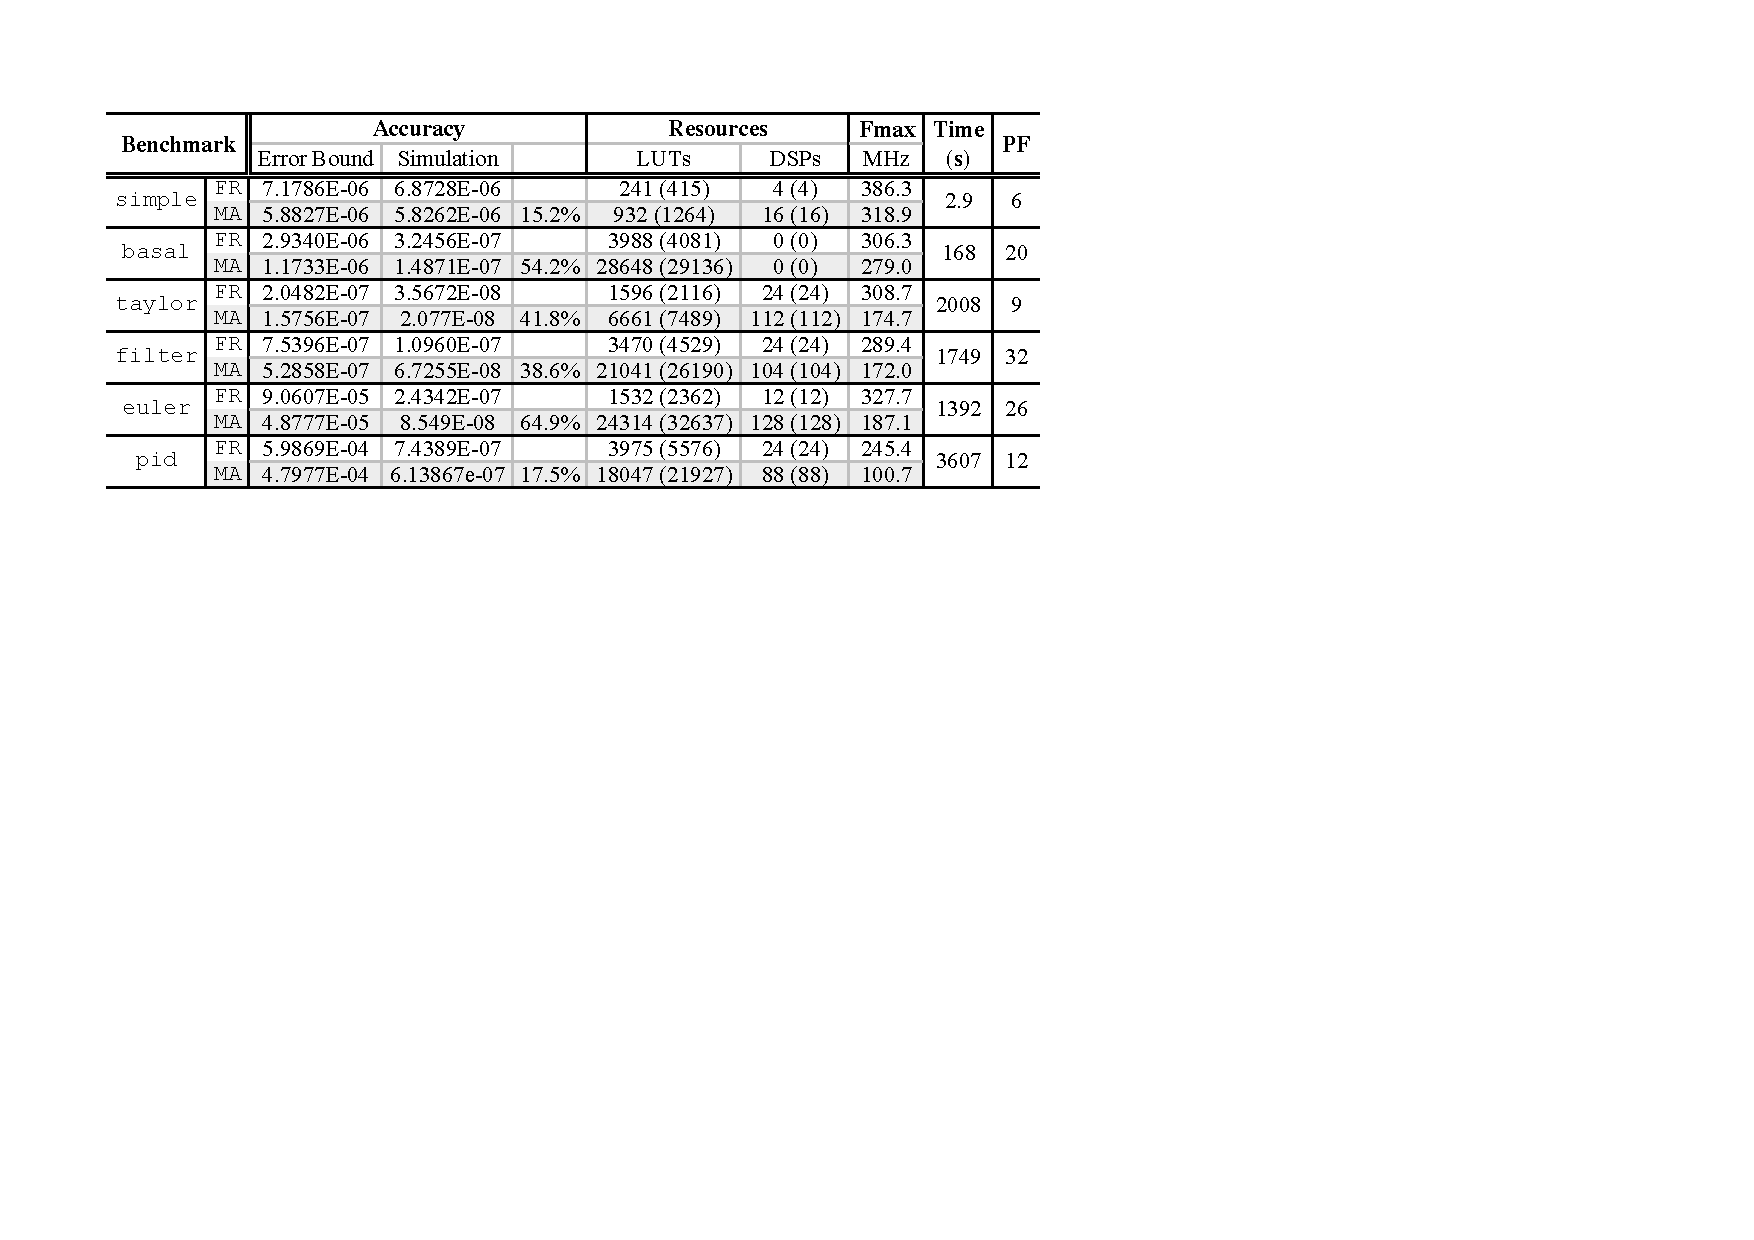
\includegraphics[width=\linewidth]{results}
    \captionof{figure}{%
    Table of optimization results.}\label{fig:results}
\end{figure}
\begin{figure}[ht]
    \centering
    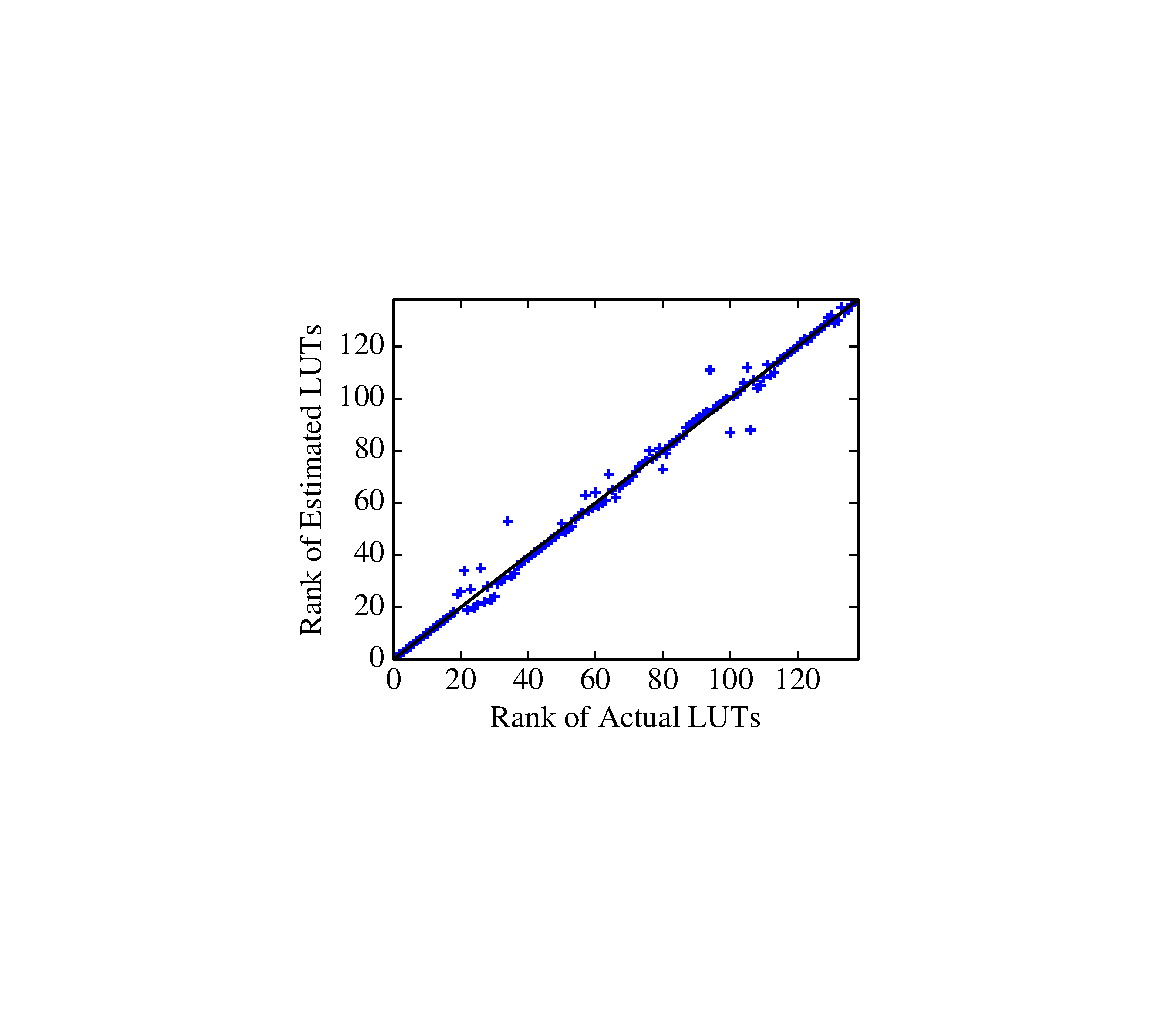
\includegraphics[scale=0.7]{rank}
    \captionof{figure}{%
    \mbox{The quality of resource estimation.}}\label{fig:rank}
\end{figure}

\begin{figure*}[ht]
    \centering
    \begin{minipage}{0.6\textwidth}
    \end{minipage}\quad\begin{minipage}{0.35\textwidth}
    \end{minipage}
\end{figure*}

The ``Resources'' columns show our estimation of the number of LUTs and
DSPs required for each of these programs, and the numbers in brackets are
the corresponding statistics obtained from Quartus synthesis.  Because
implementations on the Pareto frontier is only sensitive to how their LUTs
compare against each other, \ie~the rank, the Pareto frontier will not be
affected unless the rank is changed.  To ensure that the resource estimation
method used in our optimization can identify accurately whether an actual
implementations is on the Pareto frontier, we gathered 150 implementations
discovered across the benchmark examples, and for each one we rank its
number of estimated LUTs among them, and do the same for actual LUTs.
Figure~\ref{fig:rank} plots the rank of estimated LUTs against the rank of
actual LUTs, which shows the Pareto frontier we produced is very close to using
Quartus to count resources.

Because our benchmark examples are designed to be resource efficient, there
is no room for resource usage optimization of the original program.  However
we are able to consistently reduce the resource usage of a plain partial
loop unrolling by more than 25\%, because our optimization can discover
subexpression sharing opportunities, propagate constants values, and also
aggressively reduce the size of expressions by powerful reduction rules such as
$a - a = 0$ and $0 \times a = 0$.

Besides the choices of implementations that are either most accurate or most
resource efficient, each optimization also offers a wide selection of optimized
programs on the Pareto frontier.  For instance, Figure~\ref{fig:euler} shows
the Pareto frontier of \texttt{euler}, which has 26 different trade-off
options.  Furthermore, in the optimization of \texttt{euler}, our optimization
not only identifies that it is resource efficient when the two return variables
are computed by the same loop, but also by individually optimizing the
accuracy of the two variables, we produce a program with two loops, each with
a different goal, that is to compute their respective return variables as
accurately as possible, this generated a program that consists of two loops
that have completely different structures.  With this, we further widen the
trade-off curve with the most accurate option improving the accuracy by 65\%.
In Figure~\ref{fig:filter}, because the loop kernel of \texttt{filter} has the
expression $\sum_{i=0}^2{(a_i y_i + b_i x_i)}$, which has a large number of
equivalent expressions, without increasing the resource usage, our optimization
improves its accuracy by 14.5\%.  Because our Pareto frontier has three
dimensions, which are respectively accuracy, LUT utilization and the number of
DSPs, points within the shaded region optimize DSP count.

\begin{figure}[ht]
    \centering
    \subfloat[\texttt{euler}]{%
        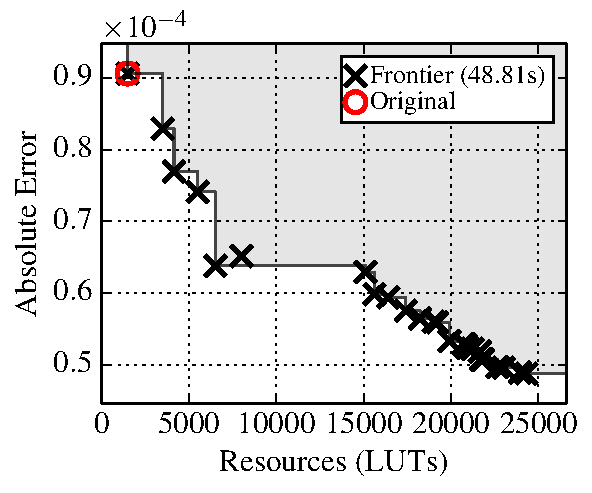
\includegraphics[width=0.6\linewidth]{euler}
        {}\label{fig:euler}
    } \\
    \subfloat[\texttt{filter}]{%
        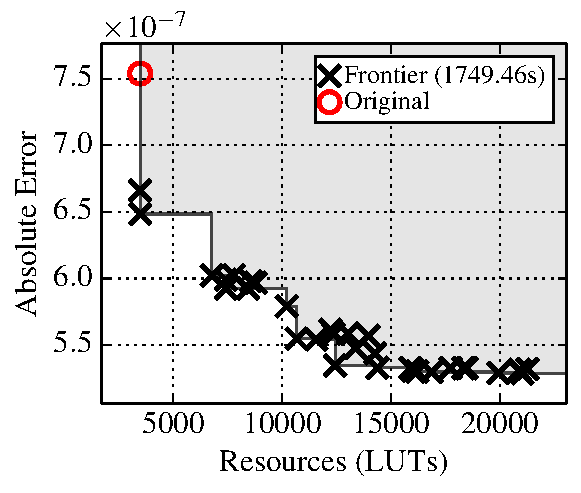
\includegraphics[width=0.6\linewidth]{filter}
        {}\label{fig:filter}
    }
    \caption{The Pareto frontier.}
\end{figure}

\section{Summary}
\label{so:sec:conclusion}

We provide a formal approach to the optimization of arithmetic expressions
for both accuracy and resource usage in high-level synthesis.  The method
proposed in this chapter and the associated tool, \soap, encompass three kind
of semantics that describe the accumulated roundoff errors, count operators in
expressions considering common subexpression elimination, and derive equivalent
expressions.  For a set of input expressions, the proposed approach works out
the respective sets of equivalent expressions in a hierarchical bottom-up
fashion, with a windowing depth limit and Pareto selection to help reduce the
complexity of equivalent expression discovery.  Using \soap, we improve either
the accuracy of our sample expressions or the resource utilization by up to
60\%, over the originals under single precision. \soap~enables a high-level
synthesis tool to optimize the structure as well as the precision of arithmetic
expressions, then to automatically choose an implementation that satisfies
accuracy and resource usage constraints.

Because we underpin our approach in formal semantics, it provides the
necessary foundation which permits us to extend the method for general
numerical program transformation in high-level synthesis.  Therefore in
Chapter~\ref{chp:progopt}, we base ourselves on the methodologies developed
in this chapter, and propose a structural approach to program optimization by
safely rewriting equivalent structures in numerical programs.



\chapter{Numerical Program Optimization}
\label{chp:progopt}

\section{Introduction}

Our previous chapter introduced a new methodology to efficiently restructure
arithmetic expressions for the optimized trade-off between two performance
metrics, \ie~numerical accuracy when evaluated and area usage in synthesized
FPGA implementations.  However, this method has a substantial limitation when
applied to general numerical programs, that is, it can only be applied to
straight-line codes without control structures such as branches and loops.

The structural optimization of general numerical programs is much more complex
than that of arithmetic expressions.  The reasons are two-fold.  First,
during program execution, variables are often updated with new values.  Our
optimization should therefore perform static analysis on the values of
variables, and use the result to optimize specifically for the trade-off
between accuracy and resource usage.  Second, it is much more difficult to
formally define program equivalence, and subsequently, to search efficiently
for optimized equivalent programs.  For instance, even without the introduction
of branches and loops, the following two programs are equivalent, but
syntactically, they are very different.  In practice, it is desirable to
eliminate as much as possible the need for these syntactic rewrites that do not
affect our performance metrics.

\begin{figure}[ht]
    \centering
    \subfloat[$P_1$]{%
        \shortstack[l]{%
            \texttt{x = x + 1;} \\
            \texttt{y = 2 * x;} \\
            \texttt{x = x + 3;}
        }
    } \qquad \qquad
    \subfloat[$P_2$]{%
        \shortstack[l]{%
            \texttt{y = x + 1;} \\
            \texttt{x = y;} \\
            \texttt{y = y * 2;} \\
            \texttt{x = x + 3;}
        }
    }
    \caption{Two programs that are equivalent but syntactically different.}
    \label{fig:equiv_progs}
\end{figure}

Therefore, in this chapter, we provide answers to these two above issues.  In
the meantime, we propose a new general \emph{program} optimization technique
for numerical algorithms, which allows \texttt{if} statements as well as
\texttt{while} loops, and developed its accompanied tool, \newsoap, to enable
the joint optimization of accuracy and resource usage, as well as the trade-off
between these performance metrics.  We develop a tool, which we call \newsoap,
to perform source-to-source optimization of numerical programs targeting FPGAs,
and generate implementations that trade off resource usage and numerical
accuracy.

% floating-point arithmetic has round-off errors, exploit equivalence

Similar to the approach we have proposed in Chapter~\ref{chp:stropt}, we
exploit equivalence rules such as such as \emph{associativity} $(a + b) +
c \equiv a + (b + c)$, and \emph{distributivity} $(a + b) \times c \equiv
a \times c + b \times c$ to automatically optimize implementations for
the optimal trade-off between resource usage, \ie~the number of LUTs and
DSP elements utilized, and accuracy when evaluated using floating-point
computations.  For example, with single precision floating-point format, our
tool found that give an input $x \in [0, 100]$ and $y \in [0, 2]$, then the
program:
\begin{lstlisting}
    if (x < 1) {
        x = (x + y) + 0.1;
    } else {
        x = x + (y + 0.1);
    }
\end{lstlisting}
is most accurate when rewritten in the following form:
\begin{lstlisting}
    if (x < 1) {
        x = (x + 0.1) + y;
    } else {
        x = x + (y + 0.1);
    }
\end{lstlisting}
On the other hand, the original program uses fewest resources when
subexpressions are shared and the \iflit~statement is eliminated:
\begin{lstlisting}
    x = x + (y + 0.1);
\end{lstlisting}

This kind of optimization generates a Pareto optimal set of implementations,
which trades off accuracy and area.  A na{\"\i}ve strategy to search for
the Pareto optimal implementations is to discover all possible equivalent
expressions.  However, this would result in combinatorial explosion and become
intractable even for very small expressions~\cite{ioualalen,mouilleron}.  To
remedy this, in Chapter~\ref{chp:stropt} we proposed a novel approach, known
as \soap, to significantly reduce the space and time complexity to produce a
subset of the Pareto frontier.

% program transformation why?

Our program optimization flow is \emph{safe}, \emph{semantics-directed} and
\emph{flexible}. \emph{Safety} means that because we make use of formal
mathematics to optimize programs, our approach can be proved correct, in
the sense that when executed using exact real arithmetic, the transformed
version produces exactly the same output values as the original program.
\emph{Semantics-directed} transformation means that not only do we use
program syntax, but also the semantics to guide optimization and guarantee
safety properties of the optimized program.  Our technique obtains when
necessary, by analyzing the program, a bound and a round-off error bound on
each variable in every program location.  These information are then used
to guide program optimization.  By analyzing and manipulating not only the
syntax, but also the semantics of programs.  The meaning of a \emph{flexible}
program transformation is three-fold.  First, arithmetic computations can be
optimized across assignments, \iflit~statements and \whilelit~loops.  Secondly,
we automatically explore the numerical implications of partial loop unrolling
and loop splitting, which can create more opportunity for minimizing round-off
errors, hence further increases range of options in the Pareto frontier of
trade-offs.  Finally, our method naturally subsumes constant propagation,
redundant code elimination, and also branch and loop fusions.

% Our tool fits in the familiar setting of the high-level synthesis tool flow, as a front-end that performs the source-to-source optimization of

Our main contributions in this chapter are as follows:
\begin{enumerate}
    \vspace{-6pt}
    \item
        A new intermediate representation of the behaviour of numerical
        programs, its structure is designed to be manipulated and analyzed
        with ease.  A new framework of numerical program transformations is
        developed to enable the back and forth translation between the program
        and a new intermediate representation (IR), which preserves the
        semantics of the original program.
    \vspace{-6pt}
    \item
        Semantics-based analyses that reason about not only the resource
        utilization (number of LUTs and DSP elements), and safe ranges of
        values and errors for programs, but also potential errors such as
        overflows and non-termination.
    \vspace{-6pt}
    \item
        A new tool, \newsoap, which trades off resource usage and accuracy
        by providing a safe, semantics-directed and flexible optimization
        targeting numerical programs for high-level synthesis.
    \vspace{-6pt}
\end{enumerate}

Section~\ref{sec:related_work} provides an overview of the existing work
related in both the software and high-level synthesis community.  We then
proceed to define our program syntax in Section~\ref{sec:syntax_definition}.
Using the syntax definition, we provide a detailed formal explanation
of our numerical program transformation, which consists of three
stages.  Section~\ref{sec:program_to_mir}, {}~\ref{sec:transformations},
{}~\ref{sec:code_generation} describe in sequence how numerical programs
can be translated into MIRs, how we infer bounds and error bounds on
variables and analyze resource usage estimates for the efficient discovery
of equivalent structures in the analyzed MIR, and finally, we explain how
a chosen MIR can be translated into an optimized numerical program.  Then
we present the optimization results in Section~\ref{sec:results} and
Section~\ref{sec:conclusion} concludes this chapter.

\section{Syntax Definition}
\label{sec:syntax_definition}

Before we discuss program transform, we first look at the syntax definition
used to write numerical programs.  Our program transformation optimizes
\numimp{} programs.  In this section, we formally introduce \numimp, a simple
imperative language which is a subset of C that supports arithmetic and Boolean
expressions, conditional branches, as well as \texttt{while} loops.  Our
language allows numerical data types $\inttype$ and $\floattype$, respectively
stand for integer and floating-point types.

We define $\aexprset, \bexprset$ as the set of arithmetic and Boolean
expressions respectively, and $\stmtset$ denotes the set of program statements.
We then have following syntax definition for expressions and \numimp{}
programs, written in the Backus-Naur Form~\cite{knuth64}:
\newcommand{\syndef}{\ensuremath\mathbin{::=}}%
\newcommand{\synor}{\ensuremath\mathbin{\mid}}%
\begin{equation}
    \begin{aligned}
        a \syndef {} &
            n \synor
            x \synor
            a_1 \odot a_2,
        \quad b \syndef x < a, \\
        s \syndef {} &
            x~\texttt{=}~a \synor
            s_1 \semicolon s_2 \synor
            \mathtt{if}~(b)~\{ s_1 \}~\mathtt{else}~\{ s_2 \} \synor
            \whilelit~(b)~\{s\}
    \end{aligned}
    \label{eq:program_syntax}
\end{equation}
We define $\odot \in \left\{ +, -, \times, / \right\}$ to be the arithmetic
operators, $n$ is a numerical constant of type either \inttype{} or \floattype;
$x \in \varset$ is a variable; $a, a_1, a_2 \in \aexprset$ are arithmetic
expressions; $b$ ranges over Boolean expressions, $\bexprset$; and similarly,
$s, s_1, s_2 \in \stmtset$ are program statements.  In our formal definition,
for the purpose of simplicity, we restrict the Boolean expressions to those
of the form $x < a$, where $x$ is a variable and $a$ is an expression;
more complex Boolean expressions are included trivially in our actual
implementation.  Although \forlit~loop is not explicitly defined in the above
syntax definition, it can be trivially derived from a \whilelit~loop.

Furthermore, we introduce the ``\verb|#pragma| \verb|soap begin|'' and
``\verb|#pragma| \verb|soap end|'' directives to delimit the code fragment
to be optimized.  We can also use ``\verb|#pragma| \verb|soap in|'' and
``\verb|#pragma| \verb|soap out|'' to provide input ranges and to declare
output variables, respectively.

As a simple example, the program in Figure~\ref{fig:syntax_example} computes an
approximate value of ${\pi^2 a}/6$.  It has two inputs $a$, a floating point
value between 0 and 1, and $n$, an integer value between 10 and 20, which
determines the number of iterations for the loop, and a return variable $y$.

\begin{figure}[ht]
    \begin{lstlisting}
    #pragma soap in \
        float a = [0.0, 1.0], int n = [10, 20]
    #pragma soap out float y
    x = 0;
    y = 0.0;
    while (x < n) {
        x = x + 1;
        y = y + a / (x * x);
    }
    \end{lstlisting}
    \caption{A simple program written with our syntax definition.}
    \label{fig:syntax_example}
\end{figure}

Despite the simplicity of our syntax, it includes all the features of
a full programming language rather than an expression language used in
Chapter~\ref{chp:stropt}.  We will add support for arrays and matrices in
Chapter~\ref{chp:latopt}, and show that this can be added with little changes
to our method.

\section{Metasemantic Intermediate Representation}
\label{po:sec:program_to_mir}

There are infinite number of ways to rewrite numerical C programs, and many of
these rewrites produce programs that have the same resource usage, accuracy and
latency characteristics.  For instance, consider the following two pairs of
programs, where each pair are equivalent, but syntactically different, as they
carry out the same (and potentially redundant) computations.
\begin{figure}[ht]
    \centering
    \newsavebox{\mirlsta}
    \begin{lrbox}{\mirlsta}
        \begin{lstlisting}
$ $
x = x + 1;
y = 2 * x;
x = x + 3;
        \end{lstlisting}
    \end{lrbox}
    \newsavebox{\mirlstb}
    \begin{lrbox}{\mirlstb}
        \begin{lstlisting}
y = x + 1;
x = y;
y = y * 2;
x = x + 3;
        \end{lstlisting}
    \end{lrbox}
    \newsavebox{\mirlstc}
    \begin{lrbox}{\mirlstc}
        \begin{lstlisting}
$ $
x = x + 1;
if ($b$)
  x = 2 * x;
        \end{lstlisting}
    \end{lrbox}
    \newsavebox{\mirlstd}
    \begin{lrbox}{\mirlstd}
        \begin{lstlisting}
if ($b$)
  x = 2*(x+1);
else
  x++;
        \end{lstlisting}
    \end{lrbox}
    \newcommand{\lstwidth}{0.25\textwidth}
    \subfloat[$P_1$]{%
        \begin{minipage}{\lstwidth}
            \usebox{\mirlsta}
        \end{minipage}
    }
    \subfloat[$P^\prime_1$]{%
        \begin{minipage}{\lstwidth}
            \usebox{\mirlstb}
        \end{minipage}
    }
    \subfloat[$P_2$]{%
        \begin{minipage}{\lstwidth}
            \usebox{\mirlstc}
        \end{minipage}
    }
    \subfloat[$P^\prime_2$]{%
        \begin{minipage}{\lstwidth}
            \usebox{\mirlstd}
        \end{minipage}
    }
    \caption{%
        Two pairs of programs that are equivalent but syntactically different.
    }\label{po:fig:equiv_progs}
\end{figure}

In practice, it is desirable to eliminate as much as possible the need for
these syntactic rewrites that do not affect our performance metrics, \eg~the
numerical accuracy and resource usage of synthesized circuits.  It is therefore
desirable to perform transformations on a \gls{dag} representation of the
program, rather than on the program text directly.  This section introduces a
new \gls{ir}, which we call the \acrfull{mir}.  It expresses how each program
variable is updated, but abstracts away the order in which the updates occur,
and ignores any temporary variables that are not marked as program outputs.

As an example, the two equivalent programs $P_1$ and $P^\prime_1$ in
Figure~\ref{po:fig:equiv_progs} can be automatically translated into an
identical \gls{mir}\@:
\begin{equation}
    \begin{tikzpicture}[mir]
        \node[mirnode] (var_x) at (0,0) {\texttt{x}};
        \node[mirnode] (plus1) [right=of var_x] {$+$};
        \node[mirnode] (n3)    [below left=of plus1] {$3$};
        \node[mirnode] (plus2) [below right=of plus1] {$+$};
        \node[mirnode] (var_y) [right=of plus1] {\texttt{y}};
        \node[mirnode] (times) [right=of var_y] {$\times$};
        \node[mirnode] (n2)    [below right=of times] {$2$};
        \node[mirnode] (x)     [below left=of plus2] {\texttt{x}};
        \node[mirnode] (n1)    [below right=of plus2] {$1$};
        \draw[|->] (var_x) -- (plus1);
        \draw[<-] (plus1) -- (n3);
        \draw[<-] (plus1) -- (plus2);
        \draw[<-] (plus2) -- (x);
        \draw[<-] (plus2) -- (n1);
        \draw[|->] (var_y) -- (times);
        \draw[<-] (times) -- (plus2);
        \draw[<-] (times) -- (n2);
        \brackets{(current bounding box)}
    \end{tikzpicture}\,.
\end{equation}

\Glspl{mir} also abstract the control structure (\ie~\iflit~branches and
\whilelit~loops) of a program, preserving only the computations that lead
to the outputs. For instance, by using the ternary conditional operator
``$\qop$'' from C, programs with conditionals such as $P_2$ and $P^\prime_2$ in
Figure~\ref{po:fig:equiv_progs} has the following \gls{mir} form:
\begin{equation}
    \begin{tikzpicture}[mir]
        \node[mirnode] (var_x) at (0,0) {\texttt{x}};
        \node[mirnode] (qop)   [right=8mm of var_x] {$\qop$};
        \node[mirnode] (b)     [below left=of qop] {$b$};
        \node[mirnode] (times) [below=6mm of qop] {$\times$};
        \node[mirnode] (n2)    [below left=of times] {$2$};
        \node[mirnode] (plus)  [below right=of times] {$+$};
        \node[mirnode] (x)     [below left=of plus] {\texttt{x}};
        \node[mirnode] (n1)    [below right=of plus] {$1$};

        \draw[|->] (var_x) -- (qop);
        \draw[<-] (qop) -- (b);
        \draw[<-] (qop) -- (times);
        \draw[<-] (times) -- (n2);
        \draw[<-] (times) -- (plus);
        \draw[<-] (plus) -- (x);
        \draw[<-] (plus) -- (n1);
        \draw[<-] (qop) to[bend left] (plus);
        \brackets{(current bounding box)}
    \end{tikzpicture}\,.
\end{equation}

This representation is useful to us, because a single \gls{mir} is able to
capture a class of syntactically-distinct programs, all of which have the
same resource usage, accuracy, and latency characteristics.  By searching for
transformations on \glspl{mir}, we drastically reduce the size of our search
space.  Note that expressions in the \gls{mir} can share common structures;
this is useful for modeling the sharing of common subexpressions and makes the
search for optimizations much more efficient.

The first step of our approach is to analyze the program return value into
a \gls{mir}\@.  This procedure is called \gls{ma}.  The \gls{ma} abstracts
away irrelevant information, and preserves the essence of program execution.
Details such as temporary variables and the ordering of program statements are
discarded, whereas the abstraction still retains data-flow dependencies and
keeps only computations that contribute to the final results.

We work with the \gls{mir} as an abstraction of the program because the
discovery of equivalent structures can be much simplified.  For instance,
the program ``\verb|x = 1; y = 2;|'' is the same as ``\verb|y = 2; x = 1;|''
because interleaving of non-dependent statements does not change program
semantics.  If we were to base our transformations on the program syntax, we
will need to enable this kind of equivalence relation even though it has zero
impact on our optimization with respect to resource usage and accuracy.  A
simpler \gls{ir} means that we can explore a much smaller search space.

Our method analyzes a program by recursively dividing the program into smaller
parts, where each part can be separately analyzed into a \gls{mir} and
composed together to form a single \gls{mir}\@.  A \gls{mir} is a mathematical
object that associates each program variable with a semantic expression.  A
semantic expression is an arithmetic expression, but with additional syntactic
features to support \iflit{} statements and \whilelit{} loops.  We represent
semantic expressions with \glspl{dag} that share common structures and define
$\sexprset$ as the set of semantic expressions, and $\mirset$ as the set of
\glspl{mir}.  Because a \gls{mir} pairs a variable with an expression, we
can view it as a function $\varset \to \sexprset$ that maps a variable into
a semantic expression.  For instance, $\mu(\varx)$ returns the associated
expression of the variable $\varx \in \varset$ for the \gls{mir} $\mu \in
\mirset$.  For each variable, its semantic expression in itself provides a
complete picture of how computations can lead to the resulting value of the
variable.  In the rest of this section, we progressively explain how each type
of program statement defined in~\eqref{po:eq:program_syntax} is analyzed into a
\gls{mir}\@.

Similar to arithmetic expressions, which can be written in a linear form
(\eg~$a + b$), or in a tree structure (\eg~\binarymir{$+$}{$a$}{$b$}),
\glspl{mir} can also be expressed in both.  The former is more concise, whereas
the latter explicitly shares common structures.

\subsection{Assignment statements}

An assignment statement is in the form of ``\texttt{x = $e$;}'', where
$\varx \in \varset$ is a program variable and $e \in \aexprset$ is an
arithmetic expression.  The metasemantic analysis of it produces a \gls{mir}
as follows:
\begin{equation}
    {\left[
        \vary \mapsto \left\{
            \begin{aligned}
                & e && \text{if~} \vary = \varx \\
                & \vary && \text{otherwise}
            \end{aligned}
        \right.
    \right]}_{\vary \in \varset}.
    \label{po:eq:mir_assign}
\end{equation}

The \gls{mir} in~\eqref{po:eq:mir_assign} signifies for a variable $\vary \in
\varset$, if $\vary$ is $\varx$, then we assign the expression $e$ to the
variable $\varx$.  In graph form, $e$ is a semantic expression represented with
a \gls{dag}\@.  The \gls{dag} shares all common subexpressions in $e$.  For
instance, an expression written as $(\varx + 1) \times (\varx + 1)$ shares the
subexpression node $\varx + 1$ by reusing the node in the \gls{dag}\@.  For
each other program variable $\vary \in \varset$, where $\vary \neq \varx$,
$\vary$ is associated with a semantic expression $\vary \in \sexprset$,
representing that the \gls{mir} does not the value of all program variables
except $\varx$, because only $\varx$ is updated in the statement.

For example, we consider a program with two variables $\varx$ and $\vary$.
Analyzing the statement ``\verb|y = x * 2;|'' produces the following \gls{mir}
graph, it is notable that the variable $\varx$ is shared between two semantic
expressions:
\begin{equation}
    \begin{tikzpicture}[mir]
        \node[mirnode] (x) at (0, 0) {\varx};
        \node[mirnode] (xexpr) [right=of x] {\varx};
        \node[coordinate] (mid) [right=of xexpr] {};
        \node[coordinate] (amid) [above=of mid] {};
        \node[mirnode] (y) [right=of mid] {\vary};
        \node[mirnode] (times) [right=of y] {$\times$};
        \node[mirnode] (two) [below right=of times] {2};

        \draw[|->] (x) -- (xexpr);
        \draw[|->] (y) -- (times);
        \draw[<-] (times) -- (two);
        \node[coordinate] (left) [below=of y] {};
        \draw[<-] (times) to[out=-135, in=0] (left);
        \draw[-] (left) to[out=180, in=-45] (amid);
        \draw[-] (amid) to[out=135, in=60] (xexpr);

        \brackets{(current bounding box)}
    \end{tikzpicture}\,.
    \label{po:eq:mir_assign_2}
\end{equation}

\subsection{Sequential statements}
\label{po:sub:sequential_statements}

A sequential statement, ``$s_1 s_2$'' is formed by joining together $s_1$
and $s_2$, where $s_1, s_2 \in \stmtset$ are statements.  It signifies that
$s_1$ and $s_2$ are executed in sequence.  Therefore, it is necessary to
\emph{append} the effect of executing $s_2$ to that of $s_1$, to arrive at the
full \gls{mir} of ``$s_1 s_2$''.  This concept can be realized by defining
a new operator $\expand$, the \emph{composition operator}, such that the
\gls{mir} of ``$s_1 s_2$'' is equal to $\mu_2 \expand \mu_1$, where $\mu_1$ and
$\mu_2$ are the \glspl{mir} of $s_1$ and $s_2$ respectively.  The resulting
\gls{mir} of $\mu_2 \expand \mu_1$ is constructed by substituting, for every
expression $e \in \sexprset$ in $\mu_2$, each variable $\varx$ in $e$ with
$\mu_1(\varx)$, which is the associated expression of $\varx$ in $\mu_1$.
Furthermore, the operator allows the format $e \expand \mu$, where $e \in
\sexprset$ is called the target expression and $\mu \in \mirset$ is the source
\gls{mir}, to mean the variables in $e$ is substituted with $\mu$ using the
composition strategy above.

We illustrate this by finding the \gls{mir} of a simple example program,
``\verb|x=x+1; y=x*2;|''.  Using the \gls{mir} of assignments, the
\glspl{mir} of the respective assignment statements can be derived, as shown
in~\eqref{po:eq:mir_seq_1}.
\begin{equation}
    \begin{tikzpicture}[mir]
        \node[mirnode] (x) at (0, 0) {\varx};
        \node[mirnode] (xexpr) [right=of x] {\varx};
        \node[coordinate] (mid) [right=of xexpr] {};
        \node[coordinate] (amid) [above=of mid] {};
        \node[mirnode] (y) [right=of mid] {\vary};
        \node[mirnode] (times) [right=of y] {$\times$};
        \node[mirnode] (two) [below right=of times] {2};

        \draw[|->] (x) -- (xexpr);
        \draw[|->] (y) -- (times);
        \draw[<-] (times) -- (two);
        \node[coordinate] (left) [below=of y] {};
        \draw[<-] (times) to[out=-135, in=0] (left);
        \draw[-] (left) to[out=180, in=-45] (amid);
        \draw[-] (amid) to[out=135, in=60] (xexpr);

        \node[coordinate] (seqleft) [right=of times, xshift=5mm] {};
        \node[mirnode] (seq) [above right=of seqleft] {$\expand$};
        \node[coordinate] (seqright) [below right=of seq] {};

        \draw[<-] (seq) -- (seqleft);
        \draw[<-] (seq) -- (seqright);

        \node[mirnode] (x2) [right=of seqright] {\varx};
        \node[mirnode] (plus2) [right=of x2] {+};
        \node[mirnode] (xto2) [below left=of plus2] {\varx};
        \node[mirnode] (one2) [below right=of plus2] {1};
        \node[coordinate] (mid2) [right=of plus2] {};
        \node[mirnode] (y2) [right=of mid2] {\vary};
        \node[mirnode] (yexpr2) [right=of y2] {\vary};

        \draw[|->] (x2) -- (plus2);
        \draw[<-] (plus2) -- (xto2);
        \draw[<-] (plus2) -- (one2);
        \draw[|->] (y2) -- (yexpr2);

        \brackets{(x) (two)};
        \brackets{(x2) (yexpr2) (one2)};
    \end{tikzpicture}\,.
    \label{po:eq:mir_seq_1}
\end{equation}
By substituting the variables with corresponding expressions, we arrive at
the \glspl{mir} as shown in~\eqref{po:eq:mir_seq_2} below.  This \gls{mir}
simplification step is always carried out when possible.
\begin{equation}
    \begin{tikzpicture}[mir]
        \node[mirnode] (x) at (0, 0) {\varx};
        \node[mirnode] (plus) [right=of x] {$+$};
        \node[mirnode] (xto) [below left=of plus] {\varx};
        \node[mirnode] (one) [below right=of plus] {1};
        \node[coordinate] (mid) [right=of plus] {};
        \node[coordinate] (amid) [above=of mid] {};
        \node[mirnode] (y) [right=of mid] {\vary};
        \node[mirnode] (times) [right=of y] {$\times$};
        \node[mirnode] (two) [below right=of times] {2};

        \draw[|->] (x) -- (plus);
        \draw[<-] (plus) -- (xto);
        \draw[<-] (plus) -- (one);
        \draw[|->] (y) -- (times);
        \draw[<-] (times) -- (two);

        \node[coordinate] (left) [below=of y] {};
        \draw[<-] (times) to[out=-135, in=0] (left);
        \draw[-] (left) to[out=180, in=-45] (amid);
        \draw[-] (amid) to[out=135, in=60] (plus);

        \brackets{(x) (two)};
    \end{tikzpicture}\,.
    \label{po:eq:mir_seq_2}
\end{equation}

\subsection{Conditional Branches}

Conditional branches, or \iflit~statements, are represented with
``\lstinline[basicstyle=\tt]|if ($b$) {$s_1$} else {$s_2$}|''.  Here $b
\in \bexprset$ is a Boolean expression, and $s_1, s_2 \in \stmtset$ are
respectively the true- and false-branches.  Our analysis of \iflit~statements
is slightly more complex, as we start to consider control flows.  The analysis
is carried out in two steps.  The first step is to compute recursively,
the \glspl{mir} $\mu_1, \mu_2 \in \mirset$ of the respective true- and
false-branches, namely, $s_1$ and $s_2$.  We introduce the conditional node
``$\qop$'' which is derived from C syntax, to signify conditional branches in
expressions.  The left-most, middle and right-most children of this node are
respectively the Boolean expression, the true- and false-expressions.  Then the
second step is to compute a new \gls{mir}, where each program variable $\varx
\in \varset$ is associated with a conditional node with three children, the
Boolean expression $b$, $\mu_1(\varx)$ and $\mu_2(\varx)$.  The final \gls{mir}
is therefore:
\begin{equation}
    {
        \left[
            \varx \mapsto \select{b}{\mu_1(\varx)}{\mu_2(\varx)}
        \right]
    }_{\varx \in \varset}.
\end{equation}

As an example, we consider the program
``\lstinline[basicstyle=\ttfamily]{if (x < 0) y = x * 2;}'', where the set
of program variables is $\{\varx, \vary\}$.  Its \gls{mir} in graph form is
therefore:
\begin{equation}
    \begin{tikzpicture}[mir]
        \node[mirnode] (x) at (0, 0) {\varx};
        \node[mirnode] (xcond) [right=of x] {$\qop$};
        \node[mirnode] (xin) [below=of xcond, yshift=-7mm] {\varx};
        \node[mirnode] (less) [below right=of xcond, xshift=5mm, yshift=-1mm]
            {$<$};
        \node[mirnode] (zero) [below right=of less, yshift=-2mm] {0};

        \node[mirnode] (y) at (25mm, 0) {\vary};
        \node[mirnode] (ycond) [right=of y] {$\qop$};
        \node[mirnode] (times) [below=of ycond] {$\times$};
        \node[mirnode] (yin) [below right=of ycond] {\vary};
        \node[mirnode] (two) [below right=of times] {2};

        \draw[|->] (x) -- (xcond);
        \draw[channel, <-] (xcond) to[out=-90, in=135] (xin);
        \draw[channel, <-] (xcond) to[out=-45, in=90] (xin);
        \draw[channel, <-] (xcond) to[out=-135, in=135] (less);
        \draw[<-] (less) -- (xin);
        \draw[channel, <-] (less) -- (zero);

        \draw[|->] (y) -- (ycond);
        \draw[<-] (ycond) to[out=-135, in=45] (less);
        \draw[<-] (ycond) -- (times);
        \draw[<-] (ycond) -- (yin);
        \draw[channel, <-] (times) -- (xin);
        \draw[channel, <-] (times) -- (two);

        \brackets{(current bounding box)};
    \end{tikzpicture}\,.
\end{equation}
Because both true- and false-expressions of $\varx$ are the same, regardless of
the truth value of $\varx < 0$, the two expressions evaluate to the same value.
In our analysis we can immediately simplify the expression of $\varx$, and the
resulting \gls{mir} is semantically equivalent to the original:
\begin{equation}
    \begin{tikzpicture}[mir]
        \node[mirnode] (x) at (0, 0) {\varx};
        \node[mirnode] (xin) [right=of x] {\varx};
        \node[mirnode] (less) [below right=of xin, xshift=3mm, yshift=-1mm]
            {$<$};
        \node[mirnode] (zero) [below right=of less, yshift=-2mm] {0};

        \node[mirnode] (y) at (25mm, 0) {\vary};
        \node[mirnode] (ycond) [right=of y] {$\qop$};
        \node[mirnode] (times) [below=of ycond] {$\times$};
        \node[mirnode] (yin) [below right=of ycond] {\vary};
        \node[mirnode] (two) [below right=of times] {2};

        \draw[|->] (x) -- (xin);
        \draw[<-] (less) to[out=-135, in=45] (xin);
        \draw[channel, <-] (less) -- (zero);

        \draw[|->] (y) -- (ycond);
        \draw[<-] (ycond) to[out=-135, in=45] (less);
        \draw[<-] (ycond) -- (times);
        \draw[<-] (ycond) -- (yin);
\begin{pgfinterruptboundingbox}
        \draw[channel, <-] (times) to[out=-135, in=60] (xin);
\end{pgfinterruptboundingbox}
        \draw[channel, <-] (times) -- (two);

        \brackets{(x) (zero) (two)};
    \end{tikzpicture}\,.
\end{equation}

The traditional approach of program abstraction uses
\glspl{cdfg}~\cite{namballa04}, which preserves the ordering of sequential
statements, uses a one-to-one mapping from assignment statements to assignment
nodes, storage nodes are used to store the result of assignments, \ie~it allows
nodes to act as a memory to store values, and finally, uses cycles in graphs
to represent program loops.  In contrast, our \glspl{mir}, from our analysis
point of view, use no local storage of temporary values, discard unnecessary
intermediate statements.  Most importantly, we treat control structures as
operators in expressions, in the same way as arithmetic computations.  In
comparison with \glspl{cdfg}, these above facts make \glspl{mir} a more
suitable candidate for exploring the search space of program transformations.

\subsection{Loops}

A possible way to represent a \whilelit~loop,
``\lstinline[basicstyle=\tt]|while ($b$) {$s$}|'', where $b \in \bexprset$
and $s \in \stmtset$, is to effectively view it as the semantic expression of
a fully unrolled loop.  Unfortunately this expression has an infinite depth,
which cannot be represented fully in a data structure.  We therefore introduce
a new operator for semantic expressions, ``$\fix$'', which we call the
\emph{fixpoint} operator.  We further use the fixpoint expression $\fix(f)$ to
represent the \whilelit~loop, where the function $f: \sexprset \to \sexprset$,
defined as $f(e_\varx) = \select{b}{e_\varx \expand \mu_s}{\varx}$, represents
the computation of one iteration of the loop, and $\mu_s$ is the \gls{mir}
of the loop body.  Finally, the fixpoint expression of a \whilelit~loop can
be written more succinctly using $lambda$-expression~\cite{barendregt13},
\ie~$\fix\left(\lambda e_\varx \dotop \select{b}{e_\varx \expand
\mu_s}{\varx}\right)$.

In graph form, for simplicity the fixpoint node admits three child nodes,
namely, the Boolean expression $b$, the loop body represented by a \gls{mir},
and the loop exit variable.  The loop body \gls{mir} can be obtained with our
\gls{ma} of the loop body, and the loop exit variable denotes which variable we
use on loop exit as the evaluated result of the fixpoint expression.  We let
$\mu_s$ to be the \gls{mir} of the loop body $s$, and derive the \gls{mir} of
the \whilelit~loop, by computing the fixpoint expression for each variable:
\begin{equation}
    {\left[
        \varx \mapsto \left\{
            \begin{aligned}
                & \fixexprmir
                    && \text{if~} \varx \in \varfunc{\mu_s} \\
                & \quad ~ ~ \varx && \text{otherwise}
            \end{aligned}
        \right.
    \right]}_{\varx \in \varset}
    \label{po:eq:mir_while}
\end{equation}
Here, $\varfunc{\mu_s}$ computes the set of variables that is assigned
in the loop body $\mu_s$.  If a program variable $\varx$ is in the set
$\varfunc{\mu_s}$, it is paired with its fixpoint expression \fixexprmir;
otherwise $\varx$ is not updated in the loop, and the loop has no effect
on its value, therefore it is paired with an expression $\varx$.  Finally,
the constructed \gls{mir} maximally shares common expressions across nested
\glspl{mir}.

As a simple example, consider the program in
Figure~\ref{po:lst:loop_share_example}.  The \gls{mir} of this example program
allows a nested \gls{mir} to reference and reuse an expression from the outer
\gls{mir} as demonstrated in Figure~\ref{po:fig:mir_fix_external_2}, where:
\begin{equation}
    \mu = [\varx \mapsto \varx + 1],
    \text{~and} \quad
    b = \varx < \vary.
\end{equation}

\begin{figure}[ht]
    \centering
    \newsavebox{\loopsharelst}
    \begin{lrbox}{\loopsharelst}
    \begin{lstlisting}
y = y + 1;
while (x < y) {
    x = x + 1;
}
    \end{lstlisting}
    \end{lrbox}
    \subfloat[The program.]{%
        \begin{minipage}{0.3\textwidth}
            \usebox{\loopsharelst}
        \end{minipage}\label{po:lst:loop_share_example}
    }
    \subfloat[The \gls{mir}.]{%
        \begin{tikzpicture}[mir]
            \node[mirnode] (x) at (0, 0) {\varx};
            \node[mirnode] (*) [right=of x] {$\expand$};
            \draw[|->] (x) -- (*);

            \node[mirnode] (fix) [below left=of *] {$\fix$};
            \node[mirnode] (b) [below left=of fix] {$b$};
            \node[mirnode] (mu) [below=of fix] {$\mu$};
            \node[mirnode] (xin) [below right=of fix] {\varx};
            \draw[<-] (*) -- (fix);
            \draw[<-] (fix) -- (b);
            \draw[<-] (fix) -- (mu);
            \draw[<-] (fix) -- (xin);

            \node[coordinate] (mir) [below right=of *] {};
            \node[mirnode] (mirx) [right=of mir, xshift=-1mm] {\varx};
            \node[mirnode] (mirxin) [right=of mirx] {\varx};
            \node[mirnode] (miry) [right=of mirxin] {\vary};
            \node[coordinate] (mirymid) [right=of miry] {};
            \node[coordinate] (miryout) [right=of mirymid] {};
            \node[coordinate] (miryedge) [right=of miryout] {};
            \draw[<-] (*) -- (mir);
            \draw[|->] (mirx) -- (mirxin);
            \draw[|->] (miry) -- (mirymid);
            \brackets{(mirx) (mirxin) (miryedge)};

            \node[mirnode] (y) [right=of *, xshift=35mm] {\vary};
            \node[mirnode] (+) [right=of y] {$+$};
            \node[mirnode] (yin) [below left=of +] {\vary};
            \node[mirnode] (1) [below right=of +] {$1$};
            \draw[|->] (y) -- (+);
            \draw[<-] (+) -- (yin);
            \draw[<-] (+) -- (1);

            \draw[<-] (miryout)
                to[out=-90, in=-180] (38mm, -7mm)
                to[out=0, in=180] (48mm, 5mm)
                to[out=0, in=135] (+);

            \brackets{(x) (b) (mu) (1)};
        \end{tikzpicture}\label{po:fig:mir_fix_external_2}
    }
    \caption{%
        A simple program which exhibits common subexpressions reuse across
        nested \glspl{mir}.
    }
\end{figure}


\subsection{Example analysis}

To illustrate all these above translation process in conjunction,
we can perform the \gls{ma} on the program \verb|basel| in
Figure~\ref{po:lst:syntax_example}.  Here, we translate it into the following
\gls{mir}, and the semantic expression for $\varx$ is omitted for simplicity:
\begin{equation}
\begin{tikzpicture}[mir]
    \node[mirnode] (x) at (0, 0) {\varx};
    \node[mirnode] (dots) [right=of x] {\textellipsis};
    \node[mirnode] (y) [right=of dots, xshift=5mm] {\vary};
    \node[mirnode] (expand) [right=of y] {$\expand$};
    \node[mirnode] (fix) [below left=of expand] {$\fix$};
    \node[mirnode] (less) [below left=of fix, xshift=-5mm] {$<$};
    \node[mirnode] (xin) [below left=of less] {\varx};
    \node[mirnode] (nin) [below right=of less] {\varn};
    \node[coordinate] (fixmir) [below=of fix, xshift=2mm, yshift=-7mm] {};
    \node[coordinate] (initmir) [right=of expand, xshift=4mm] {};
    \node[mirnode] (yin) [below right=of fix] {\vary};
    \node[mirnode] (a) [right=of expand, xshift=40mm] {\vara};
    \node[mirnode] (ain) [right=of a] {\vara};
    \node[mirnode] (n) [right=of ain] {\varn};
    \node[mirnode] (nin2) [right=of n] {\varn};
    \draw[|->] (x) -- (dots);
    \draw[|->] (y) -- (expand);
    \draw[|->] (a) -- (ain);
    \draw[|->] (n) -- (nin2);
    \draw[<-] (expand) -- (fix);
    \draw[<-] (fix) -- (less);
    \draw[<-] (less) -- (xin);
    \draw[<-] (less) -- (nin);
    \draw[<-] (fix) -- (fixmir);
    \draw[<-] (fix) -- (yin);
    \draw[<-] (expand) to[out=-45, in=135] (initmir);

    \node[mirnode] (fixx) [below=of fixmir, xshift=1mm, yshift=2mm] {\varx};
    \node[mirnode] (fixadd1) [right=of fixx] {$+$};
    \node[mirnode] (fixxin) [below left=of fixadd1] {\varx};
    \node[mirnode] (fixone) [below right=of fixadd1] {1};
    \node[mirnode] (fixy) [right=of fixadd1, xshift=5mm] {\vary};
    \node[mirnode] (fixadd2) [right=of fixy] {$+$};
    \node[mirnode] (fixyin) [below left=of fixadd2] {\vary};
    \node[mirnode] (fixdiv) [below right=of fixadd2] {$/$};
    \node[mirnode] (fixmul) [below right=of fixdiv] {$\times$};
    \node[coordinate] (fixmulin1) [left=of fixmul, xshift=-13mm] {};
    \node[coordinate] (fixmulin2) [right=of fixadd2, xshift=5mm] {};
    \node[coordinate] (fixmuledge) [right=of fixmul, xshift=-2.1mm] {};
    \node[mirnode] (fixa) [below=of fixx, yshift=-10mm] {\vara};
    \node[mirnode] (fixain) [right=of fixa] {\vara};
    \draw[|->] (fixx) -- (fixadd1);
    \draw[<-] (fixadd1) -- (fixxin);
    \draw[<-] (fixadd1) -- (fixone);
    \draw[|->] (fixy) -- (fixadd2);
    \draw[<-] (fixadd2) -- (fixyin);
    \draw[<-] (fixadd2) -- (fixdiv);
    \draw[<-] (fixdiv) -- (fixmul);
    \draw[<-] (fixmul) to[out=-135, in=-45] (fixmulin1);
    \draw[-] (fixmulin1) to[out=135, in=45] (fixadd1);
    \draw[<-] (fixmul) to[out=-45, in=-45] (fixmulin2);
    \draw[-] (fixmulin2) to[out=135, in=55] (fixadd1);
    \draw[|->] (fixa) -- (fixain);
    \draw[channel, <-] (fixdiv) to[out=-135, in=45] (fixain);
    \brackets{(fixx) (fixa) (fixmuledge)};

    \node[mirnode] (initx) [below=of initmir, xshift=2mm, yshift=2mm] {\varx};
    \node[mirnode] (initzero1) [right=of initx] {$0$};
    \node[mirnode] (inity) [below=of initx] {\vary};
    \node[mirnode] (initzero2) [right=of inity] {$0.0$};
    \node[mirnode] (inita) [right=of initzero1, xshift=5mm] {\vara};
    \node[mirnode] (initain) [right=of inita] {\vara};
    \node[mirnode] (initn) [below=of inita] {\varn};
    \node[mirnode] (initnin) [right=of initn] {\varn};
    \draw[|->] (initx) -- (initzero1);
    \draw[|->] (inity) -- (initzero2);
    \draw[|->] (inita) -- (initain);
    \draw[|->] (initn) -- (initnin);
    \brackets{(initx) (initnin)};

    \brackets{(current bounding box)};
\end{tikzpicture}\,.
\end{equation}

\section{Accuracy Analysis}
\label{so:sec:accuracy}

The accuracy analysis used by \soap{} follows the method based on abstract
error domain introduced by Martel~\cite{martel07} to analyze the round-off
error of restructured floating-point expressions.  As it was mentioned in
Section~\ref{bg:ssub:accuracy}, they did not have a preference for the choice
of definition of $\ulp$.  Hence, here we propose to use a definition of $\ulp$
derived from the standard IEEE 754 floating-point representation.

To begin, the concepts of the floating-point representation~\cite{ieee754}
should be introduced.  Any values $v$ representable in floating-point with
standard exponent offset can be expressed with the format given by the
following equation:
\begin{equation}
    v = s \times 2^{e - (2^{k - 1} - 1)} \times 1.{m_1 m_2 m_3 \ldots m_p}.
    \label{bg:eq:floating_point}
\end{equation}
In~\eqref{bg:eq:floating_point}, the bit $s$ is the sign bit, the $k$-bit
unsigned integer $e$ is known as the exponent bits, and the $p$-bits $m_1 m_2
m_3 \ldots m_p$ are the mantissa bits, here we use $1.{m_1 m_2 m_3 \ldots m_p}$
to indicate a fixed-point number represented in unsigned binary format.

Note that a non-zero floating-point with the smallest magnitude can be found
by setting $e = 0$ and $m_1, m_2, \ldots, m_p$ to $0$, which may still be far
away from $0$ when compared to the next non-zero floating-point value, where
$e = 0$, $m_1, m_2, \ldots, m_{p-1}$ are all $0$, and $m_p = 1$.  To solve
this discontinuous behaviour, extra logic can be used to allow a different
floating-point representation when $e = 0$:
\begin{equation}
    v = s \times 2^{-(2^{k-1} - 1)} \times 0.{m_1 m_2 m_3 \ldots m_p}.
\end{equation}
This alternative behaviour is known as gradual underflow, whereas the original
is abrupt underflow.

In \soap{}, the distance between two adjacent floating-point values $f_1$ and
$f_2$ satisfying $f_1 \leq x \leq f_2$ for a value $x$~\cite{goldberg} is known
as the \emph{unit of the last place} function $\ulp(x)$.  To characterize
this function, we further restrict that $f_1$ and $f_2$ must not equal and
no other floating-point values exists between them.  We can now provide the
definition for $\ulp(x)$, where GU and AU respectively indicate gradual and
abrupt underflow modes:
\begin{definition}
    In our analysis, the function $\ulp(x)$ is defined as:
    \begin{equation}
        \ulp(x) = \left\{
            \begin{aligned}
                & \infty,  && \text{if $x$ is $-\infty$ or $\infty$}, \\
                & 2^{e(x) - (2^{k - 1} - 1)} \times 2^{-p},
                \quad && \text{%
                    if GU and $x$ is not $-\infty$ or $\infty$
                }, \\
                & \max\left(
                    2^{-(2^{k-1} - 1)},
                    2^{e(x) - (2^{k - 1} - 1)} \times 2^{-p}
                \right) \quad && \text{%
                    if AU and $x$ is not $-\infty$ or $\infty$
                }.
            \end{aligned}
        \right.
    \end{equation}
    where $e(x)$ is the exponent of $x$, $k$ and $p$ are the parameters of the
    floating-point format as defined in~\eqref{bg:eq:floating_point}.
    {}\label{so:def:ulp}
\end{definition}

Since Martel~\cite{martel07} does not define the arithmetic operator for
division.  The following equations for division are therefore introduced in
this thesis.  Firstly, divisions on intervals can be implemented as follows:
\begin{equation}
    \frac{\interval{a}{b}}{\interval{c}{d}}
        \defeq \interval{\min(s)}{\max(s)},
\end{equation}
where $\interval{a}{b}, \interval{c}{d} \in \intervalset$ and:
\begin{equation}
    s = \left\{
    \begin{aligned}
        & \{ -\infty, \infty \}
            && \text{if~} c \leq 0 \leq d, \\
        & \left\{
            \frac{a}{c}, \frac{a}{d}, \frac{b}{c}, \frac{b}{d}
        \right\}
            \quad && \text{otherwise}.
    \end{aligned}
    \right.
\end{equation}
By evaluating the sum of error propagated $\frac{ x^\sharp_1 + \mu^\sharp_1 }{
x^\sharp_2 + \mu^\sharp_2 } - \frac{x^\sharp_1}{x^\sharp_2}$ and the round-off
error introduced by division, the division on values in the abstract error
domain can be derived as follows:
\begin{equation}
    \frac{
        \left( x^\sharp_1, \mu^\sharp_1 \right)
    }{
        \left( x^\sharp_2, \mu^\sharp_2 \right)
    }
    \defeq \left(
            \roundup{\frac{x^\sharp_1}{x^\sharp_2}},
            \frac{
                x^\sharp_2 \mu^\sharp_1 - x^\sharp_1 \mu^\sharp_2
            }{
                x^\sharp_2 \left( x^\sharp_2 + \mu^\sharp_2 \right)
            } + \rounddown{\frac{x^\sharp_1}{x^\sharp_2}}
        \right).
\end{equation}
Recall from Section~\ref{bg:ssub:accuracy} of Chapter~\ref{chp:background},
$\roundup{\frac{x^\sharp_1}{x^\sharp_2}}$ computes the range of floating-point
values by rounding values in $\frac{x^\sharp_1}{x^\sharp_2}$, and
$\rounddown{\frac{x^\sharp_1}{x^\sharp_2}}$ returns the range of errors
introduced in the rounding process.

We use the function $\error: \aexprset\to\errorset$ to represent the
analysis of round-off error in an expression tree, as described in
Section~\ref{bg:ssub:accuracy} of Chapter~\ref{chp:background}, using the above
$\ulp$ equation in Definition~\ref{so:def:ulp}, where $\aexprset$ denotes the
set of all arithmetic expressions.

For each expression in a set of equivalent expressions discovered, $e \in
\epsilon$, each expression $e$ evaluates to a distinct value in the abstract
error domain.  Section~\ref{bg:ssub:accuracy} of Chapter~\ref{chp:background}
presents a method to compare against each other with a partial ordering.
However, a total ordering is much more preferable, as all expressions can
be easily compared against one another.  In \soap, the following function
$\abserr$ is used to convert an evaluated outcome $v \in \errorset$ into a
scalar to denote the magnitude of round-off error:
\begin{equation}
    \abserr(e) = \max\left(
        \left| \mu^\sharp_{\min} \right|,
        \left| \mu^\sharp_{\max} \right|
    \right),
    \quad \text{where~}
    \left(
        x^\sharp, \left[ \mu^\sharp_{\min}, \mu^\sharp_{\max} \right]
    \right) = \error(e).
    \label{so:eq:abserr}
\end{equation}

\section{Resource Usage Analysis}
\label{po:sec:resource}

In this section we give a detailed explanation of how resources in \glspl{mir}
can be shared and how to analyze the resource utilization of \glspl{mir}.

Expressions can have common subexpressions, and eliminating them reduces
resource usage.  We identify and eliminate common subexpressions when we
construct \glspl{dag} from programs.  Resource statistics can be estimated
by accumulating \gls{lut} and \gls{dsp} counts of each operator in the
\gls{dag}\@.  However, we can further merge multiple nodes into one to reduce
the estimated resource usage of generated code.  Conventional compiler
optimizations~\cite{kuck81} such as branch and loop fusion, as well as
redundant code elimination can be applied in an equivalent fashion to our
\glspl{mir} to share conditional and fixpoint operators.  This process further
reintroduces control structures to \glspl{mir}, so that the code generation
stage can make use of the result to synthesize code without redundant control
structures.


\subsection{Sharing conditional expressions}

In its essence, the sharing of the conditional operator is equivalent to
branch fusion.  For example, we consider the \gls{mir} of the program in
Figure~\ref{po:lst:branch_example}.  The \gls{ma} of it produces the \gls{mir}
in Figure~\ref{po:fig:mir_cond_fusion_1}.

\begin{figure}[ht]
    \centering
    \newsavebox{\branchfusionlst}
    \begin{lrbox}{\branchfusionlst}
    \begin{lstlisting}
if (x < 0) {
    x = 1;
    y = 2;
} else {
    x = 3;
    y = 4;
}
    \end{lstlisting}
    \end{lrbox}
    \subfloat[The program.]{%
        \begin{minipage}{0.25\textwidth}
            \usebox{\branchfusionlst}
        \end{minipage}\label{po:lst:branch_example}
    }
    \subfloat[Before fusion.]{%
        % \includegraphics[scale=\mirfigscale]{mir_cond_fusion_1}
        \begin{tikzpicture}[mir]
            \node[mirnode] (x) at (0, 0) {\varx};
            \node[mirnode] (xq) [right=of x] {$\qop$};
            \node[mirnode] (1) [below=of xq, yshift=-2mm, inner sep=2mm] {$1$};
            \node[mirnode] (3)
                [below right=of xq, yshift=-2mm, inner sep=1mm] {$3$};

            \node[coordinate] (mid) [right=of xq, xshift=13mm] {};
            \node[mirnode] (y) [right=of mid, xshift=5mm] {\vary};
            \node[mirnode] (yq) [right=of y] {$\qop$};
            \node[mirnode] (2) [below=of yq, inner sep=2mm] {$2$};
            \node[mirnode] (4) [below right=of yq, inner sep=1mm] {$4$};

            \node[mirnode] (<) [below=of mid, yshift=-2mm] {$<$};
            \node[mirnode] (xin) [below left=of <] {\varx};
            \node[mirnode] (0) [below right=of <] {$0$};

            \draw[|->] (x) -- (xq);
            \draw[|->] (y) -- (yq);
            \draw[<-] (xq) to[out=-135, in=135] (<);
            \draw[<-] (yq) to[out=-135, in=45] (<);
            \draw[channel,-] (xq) -- (1);
            \draw[channel,-] (xq) -- (3);
            \draw[<-] (yq) -- (2);
            \draw[<-] (yq) -- (4);
            \draw[<-] (<) -- (xin);
            \draw[<-] (<) -- (0);

            \brackets{(current bounding box)};
        \end{tikzpicture}\label{po:fig:mir_cond_fusion_1}
    }\quad
    \subfloat[After fusion.]{%
        % \includegraphics[scale=\mirfigscale]{mir_cond_fusion_2}
        \begin{tikzpicture}[mir]
            \node[mirnode] (x) at (0, 0) {\varx};
            \node[coordinate] (xmid) [right=of x] {};
            \node[coordinate] (xout) [right=of xmid] {};
            \node[coordinate] (mid) [right=of xout] {};
            \node[mirnode] (y) [right=of mid] {\vary};
            \node[coordinate] (ymid) [right=of y] {};
            \node[coordinate] (yout) [right=of ymid] {};
            %\node[coordinate] (yedge) [right=of yout] {};

            \node[coordinate] (out) [below=of mid, yshift=-2mm] {};
            \node[mirnode, inner sep=2mm] (?) [below=of out] {$\qop$};
            \node[mirnode] (<) [below left=of ?, xshift=-10mm, yshift=2mm] {$<$};
            \node[coordinate] (in1) [below=of ?, yshift=-3mm] {};
            \node[coordinate] (in2) [below right=of ?, xshift=10mm] {};

            \node[mirnode] (xin) [below left=of <] {\varx};
            \node[mirnode] (0) [below right=of <] {0};
            \node[mirnode] (1) [below left=of in1] {1};
            \node[mirnode] (2) [below right=of in1] {2};
            \node[mirnode] (3) [below left=of in2] {3};
            \node[mirnode] (4) [below right=of in2] {4};

            \draw[|->] (x) -- (xmid);
            \draw[|->] (y) -- (ymid);
            \draw[<-] (yout) to[out=-90, in=45] (out);
            \draw[<-] (xout) to[out=-90, in=135] (out);
            \draw[o] (?) -- (out);

            \draw[<-] (?) -- (<);
            \draw[<-] (<) -- (xin);
            \draw[<-] (<) -- (0);
            \draw[<-] (?) -- (in1);
            \draw[<-] (?) -- (in2);
            \draw[-] (1) -- (in1);
            \draw[o] (2) -- (in1);
            \draw[-] (3) -- (in2);
            \draw[o] (4) -- (in2);

            \brackets{(current bounding box)};
        \end{tikzpicture}\label{po:fig:mir_cond_fusion_2}
    }
    \caption{The sharing of conditional expressions in a simple program.}
\end{figure}

Because we compute an abstraction of the program, the \gls{mir} does not
keep the structure of the \iflit~statement to allow them to be optimized
separately, as doing this would allow our optimization to produce more accurate
implementations.  The resulting \gls{mir} of the program consists of two
conditional expressions as shown in Figure~\ref{po:fig:mir_cond_fusion_1}.
Because of this, after optimization, the \gls{mir} may has duplicate control
paths.  To resolve this, we introduce new kinds of nodes, as shown in
Figure~\ref{po:fig:mir_cond_fusion_2}, to ``bundle up'' more than one
conditional expressions, when they all have the same Boolean expression.


\subsection{Resource sharing in composition expressions}

Composition expressions can be fused in an analogous manner.  Any \glspl{mir}
$\mu_1$ and $\mu_2$ can be merged to form a new \gls{mir} if there are no
conflicts in the variable-expression pairing, \ie~for any variable $x$ that
is assigned an expression in both $\mu_1$ and $\mu_2$, $\mu_1(x)$ is equal
to $\mu_2(x)$.  A ``bundle'' of expressions can also be created to denote
the sharing of the composition operator.  For example, a simple \gls{mir}
in Figure~\ref{po:fig:mir_sub_fusion_1} can be restructured by fusing both
variables $x$ and $y$.
\begin{figure}[ht]
    \centering
    \subfloat[Before fusion.]{%
        % \includegraphics[scale=\mirfigscale]{mir_sub_fusion_1}
        \begin{tikzpicture}[mir]
            \node[mirnode] (x) at (0, 0) {\varx};
            \node[mirnode] (x*) [right=of x] {$\expand$};
            \node[coordinate] (mid) [right=of x*, xshift=10mm] {};
            \node[mirnode] (y) [right=of mid] {\vary};
            \node[mirnode] (y*) [right=of y] {$\expand$};

            \node[mirnode] (xin) [below left=of x*] {\varx};
            \node[mirnode] (xmir) [below right=of x*] {};
            \node[mirnode] (zin) [below left=of y*] {\varz};
            \node[mirnode] (zmir) [below right=of y*] {};

            \draw[<-] (x*) -- (xin);
            \draw[<-] (x*) -- (xmir);
            \draw[<-] (y*) -- (zin);
            \draw[<-] (y*) -- (zmir);

            \node[mirnode] (xmirx) [below=of x*] {\varx};
            \node[mirnode] (xmir+) [right=of xmirx] {$+$};
            \node[mirnode] (xmirxin) [below left=of xmir+] {\varx};
            \node[mirnode] (xmir1) [below right=of xmir+] {$1$};
            \draw[|->] (xmirx) -- (xmir+);
            \draw[<-] (xmir+) -- (xmirxin);
            \draw[<-] (xmir+) -- (xmir1);
            \brackets{(xmirx) (xmir1)};

            \node[mirnode] (zmirz) [below=of y*] {\varz};
            \node[mirnode] (zmir*) [right=of zmirz] {$\times$};
            \node[mirnode] (zmirxin) [below right=of zmir*] {\varx};
            \node[mirnode] (zmirzin) [below left=of zmir*] {\varz};
            \draw[|->] (zmirz) -- (zmir*);
            \draw[<-] (zmir*) -- (zmirzin);
            \draw[<-] (zmir*) -- (zmirxin);
            \brackets{(zmirz) (zmirxin)};

            \draw[|->] (x) -- (x*);
            \draw[|->] (y) -- (y*);

            \brackets{(current bounding box)};
        \end{tikzpicture}\label{po:fig:mir_sub_fusion_1}
    }\quad
    \subfloat[After fusion.]{%
        % \includegraphics[scale=\mirfigscale]{mir_sub_fusion_2}
        \begin{tikzpicture}[mir]
            \node[mirnode] (x) at (0, 0) {\varx};
            \node[coordinate] (xmid) [right=of x] {};
            \node[coordinate] (xout) [right=of xmid] {};
            \node[coordinate] (mid) [right=of xout] {};
            \node[mirnode] (y) [right=of mid] {\vary};
            \node[coordinate] (ymid) [right=of y] {};
            \node[coordinate] (yout) [right=of ymid] {};
            \draw[|->] (x) -- (xmid);
            \draw[|->] (y) -- (ymid);

            \node[coordinate] (out) [below right=of xout, yshift=-2mm] {};
            \node[mirnode] (*) [below=of out] {$\expand$};
            \draw[<-] (xout) -- (out);
            \draw[<-] (yout) to[out=-90, in=45] (out);
            \draw[o] (*) -- (out);

            \node[coordinate] (lin) [below left=of *] {};
            \node[coordinate] (mir) [below right=of *] {};
            \node[mirnode] (xin) [below left=of lin] {\varx};
            \node[mirnode] (zin) [below right=of lin] {\varz};
            \draw[<-] (*) -- (lin);
            \draw[-] (xin) -- (lin);
            \draw[o] (zin) -- (lin);
            \draw[<-] (*) -- (mir);

            \node[mirnode] (mirz) [right=of *] {\varz};
            \node[mirnode] (mir*) [right=of mirz] {$\times$};
            \node[mirnode] (mirx) [right=of mir*] {\varx};
            \node[mirnode] (mir+) [right=of mirx] {$+$};
            \node[mirnode] (mirzin) [below left=of mir*] {\varz};
            \node[mirnode] (mirxin) [below left=of mir+] {\varx};
            \node[mirnode] (mir1) [below right=of mir+] {$1$};
            \draw[|->] (mirz) -- (mir*);
            \draw[|->] (mirx) -- (mir+);
            \draw[<-] (mir*) -- (mirzin);
            \draw[<-] (mir*) -- (mirxin);
            \draw[<-] (mir+) -- (mirxin);
            \draw[<-] (mir+) -- (mir1);
            \brackets{(mirz) (mir1)};

            \brackets{(current bounding box)};
        \end{tikzpicture}\label{po:fig:mir_sub_fusion_2}
    }
    \caption{The sharing of composition expressions.}
\end{figure}


\subsubsection{Resource sharing in fixpoint expressions}

For fixpoint expressions that represent \whilelit~loops, discovering resource
sharing opportunities is a little more complex.  We fuse fixpoint expressions
in an analogous fashion as described above for conditional expressions, and
it is related to the conventional loop fusion compiler optimization.  For
instance, the program in Figure~\ref{po:lst:loop_example} has the \gls{mir}
in Figure~\ref{po:fig:mir_fix_fusion_1}, where:
\begin{equation}
    b = \varx > \vary, \quad
    \mu_1 = [\varx \mapsto \varx / 2], \text{~and} \quad
    \mu_2 = [\varx \mapsto \varx / 2, \varz \mapsto \varz + \varx].
\end{equation}

During program optimization, the two fixpoint expressions are optimized
individually, because loop splitting could enhance the accuracy of both $x$ and
$z$.  After this, in the resulting \gls{mir}, fixpoint expressions may or may
not share computations.  The fixpoint expressions can often be fused together
to save resources in the conditional expressions and the control logic that
are formerly duplicated, if they share common computations that can be merged
without conflict.  For instance, Figure~\ref{po:fig:mir_fix_fusion_2} shows how
two expressions can be fused into one fixpoint expression.
\begin{figure}[ht]
    \centering
    \newsavebox{\loopfusionlst}
    \begin{lrbox}{\loopfusionlst}
    \begin{lstlisting}
while (x > y) {
    z = z + x;
    x = x / 2;
}
    \end{lstlisting}
    \end{lrbox}
    \subfloat[The program.]{%
        \begin{minipage}{0.26\textwidth}
            \usebox{\loopfusionlst}
        \end{minipage}\label{po:lst:loop_example}
    }
    \subfloat[Before fusion.]{%
        \begin{tikzpicture}[mir]
            \node[mirnode] (x) at (0, 0) {\varx};
            \node[mirnode] (xfix) [right=of x] {$\fix$};
            \node[mirnode] (b1) [below left=of xfix] {$b$};
            \node[mirnode] (mu1) [below=of xfix] {$\mu_1$};
            \node[mirnode] (xin) [below right=of xfix] {\varx};

            \node[mirnode] (z) [right=of xfix, xshift=5mm] {\varz};
            \node[mirnode] (zfix) [right=of z] {$\fix$};
            \node[mirnode] (b2) [below left=of zfix] {$b$};
            \node[mirnode] (mu2) [below=of zfix] {$\mu_2$};
            \node[mirnode] (zin) [below right=of zfix] {\varz};

            \node[mirnode] (y) [right=of zfix, xshift=5mm] {\vary};
            \node[mirnode] (yin) [right=of y] {\vary};

            \draw[|->] (x) -- (xfix);
            \draw[|->] (z) -- (zfix);
            \draw[|->] (y) -- (yin);
            \draw[<-] (xfix) -- (b1);
            \draw[<-] (xfix) -- (mu1);
            \draw[<-] (xfix) -- (xin);
            \draw[<-] (zfix) -- (b2);
            \draw[<-] (zfix) -- (mu2);
            \draw[<-] (zfix) -- (zin);

            \brackets{(current bounding box)};
        \end{tikzpicture}\label{po:fig:mir_fix_fusion_1}
    } \quad
    \subfloat[After fusion.]{%
        \begin{tikzpicture}[mir]
            \node[mirnode] (x) at (0, 0) {\varx};
            \node[coordinate] (xmid) [right=of x] {};
            \node[coordinate] (xout) [right=of xmid] {};

            \node[mirnode] (z) [right=of xout, xshift=5mm] {\varz};
            \node[coordinate] (zmid) [right=of z] {};
            \node[coordinate] (zout) [right=of zmid] {};

            \node[mirnode] (y) [right=of zout, xshift=5mm] {\vary};
            \node[mirnode] (yin) [right=of y] {\vary};

            \node[coordinate] (out) [below right=of xout, yshift=-2mm] {};
            \node[mirnode] (fix) [below=of out] {$\fix$};
            \draw[<-] (xout) -- (out);
            \draw[<-] (zout) to[out=-90, in=45] (out);
            \draw[o] (fix) -- (out);

            \node[mirnode] (b) [below left=of fix] {$b$};
            \node[mirnode] (mu) [below=of fix] {$\mu_2$};
            \node[coordinate] (in) [below right=of fix, xshift=5mm] {};
            \node[mirnode] (xin) [below left=of in] {\varx};
            \node[mirnode] (zin) [below right=of in] {\varz};
            \draw[<-] (fix) -- (b);
            \draw[<-] (fix) -- (mu);
            \draw[<-] (fix) -- (in);
            \draw[-] (xin) -- (in);
            \draw[o] (zin) -- (in);

            \draw[|->] (x) -- (xmid);
            \draw[|->] (z) -- (zmid);
            \draw[|->] (y) -- (yin);

            \brackets{(current bounding box)};
        \end{tikzpicture}\label{po:fig:mir_fix_fusion_2}
    }
    \caption{%
        The sharing of fixpoint expressions in a simple example program.
    }
\end{figure}

However in some cases the above transformations could create cyclic graphs.  To
illustrate this, consider the following conditional expression fusion example
in Figure~\ref{po:fig:mir_cond_fusion_3}.  By fusing both conditionals $a$ and
$b$, a cycle is created as in Figure~\ref{po:fig:mir_cond_fusion_4}.
\begin{figure}[ht]
    \centering
    \subfloat[Before fusion, the \gls{mir} is acyclic.]{%
        % \includegraphics[scale=\mirfigscale]{mir_cond_fusion_3}
        \begin{minipage}{0.35\textwidth}
        \centering
        \begin{tikzpicture}[mir]
            \node[mirnode] (x) at (0, 0) {\varx};
            \node[mirnode] (x?) [right=of x] {$\qop$};
            \node[mirnodealt] (x?2) [below=of x?] {$\qop$};
            \node[mirnode] (xin) [below right=of x?] {\varx};
            \node[mirnodealt] (1)
                [below right=of x?2, xshift=-3mm, yshift=-1mm] {$1$};
            \node[mirnodealt] (2) [below right=of x?2] {$2$};
            \node[mirnodealt] (a) [below=of x?2, yshift=-8mm] {$a$};

            \node[mirnode] (y) [right=of x?] {\vary};
            \node[mirnode] (y?) [right=of y] {$\qop$};
            \node[mirnodealt] (y?2) [below=of y?] {$\qop$};
            \node[mirnode] (yin) [below right=of y?] {\vary};
            \node[mirnodealt] (3)
                [below right=of y?2, xshift=-3mm, yshift=-1mm] {$3$};
            \node[mirnodealt] (4) [below right=of y?2] {$4$};
            \node[mirnodealt] (b) [below=of y?2, yshift=-7mm] {$b$};
            \node[coordinate] (x?2-b) [above left=of b, xshift=-4mm] {};

            \draw[|->] (x) -- (x?);
            \draw[<-] (x?) -- (x?2);
            \draw[<-] (x?) -- (xin);
            \draw[<-] (x?2) -- (1);
            \draw[<-] (x?2) -- (2);

            \draw[|->] (y) -- (y?);
            \draw[<-] (y?) -- (y?2);
            \draw[<-] (y?) -- (yin);
            \draw[<-] (y?2) -- (3);
            \draw[<-] (y?2) -- (4);

            \draw[<-] (x?) to[out=-135, in=135] (a);
            \draw[<-] (x?2) to[out=-135, in=-180] (x?2-b);
            \draw[-] (x?2-b) to[out=0, in=135] (b);
            \draw[<-] (y?) to[out=-135, in=120] (b);
            \draw[channel,<-] (y?2) to[out=-120, in=45] (a);

            \brackets{(current bounding box)};
        \end{tikzpicture}
        \end{minipage}\label{po:fig:mir_cond_fusion_3}
    }\quad
    \subfloat[%
        Fusing the two conditional operators $a$ and $b$ creates a cycle.
    ]{%
        % \includegraphics[scale=\mirfigscale]{mir_cond_fusion_4}
        \begin{tikzpicture}[mir]
            \node[mirnode] (x) at (0, 0) {\varx};
            \node[coordinate] (xmid) [right=of x] {};
            \node[coordinate] (xout) [right=of xmid] {};
            \node[mirnode] (y) [right=of xout, xshift=15mm] {\vary};
            \node[coordinate] (ymid) [right=of y] {};
            \node[coordinate] (yout) [right=of ymid] {};
            \draw[|->] (x) -- (xmid);
            \draw[|->] (y) -- (ymid);

            \node[coordinate] (o1) [below right=of xout] {};
            \node[mirnodealt] (?1) [below left=of o1] {$\qop$};
            \node[mirnode] (a) [below left=of ?1] {$a$};
            \node[coordinate] (i1) [below=of ?1, yshift=-3mm, xshift=-3mm] {};
            \node[coordinate] (i2) [below right=of ?1, xshift=2mm] {};
            \node[mirnode] (3) [below right=of i1] {$3$};
            \node[mirnode] (xin) [below left=of i2] {\varx};
            \node[mirnode] (4) [below right=of i2] {$4$};

            \node[coordinate] (o2) [below left=of y] {};
            \node[mirnodealt] (?2) [below right=of o2] {$\qop$};
            \node[mirnode] (b) [below left=of ?2] {$b$};
            \node[coordinate] (i3) [below=of ?2, xshift=5mm] {};
            \node[coordinate] (i4) [below right=of ?2, xshift=10mm] {};
            \node[mirnode] (1) [below left=of i3] {$1$};
            \node[mirnode] (2) [below left=of i4] {$2$};
            \node[mirnode] (yin) [below right=of i4] {\vary};

            \draw[-, red] (o1) -- (?1);
            \draw[<-, red] (?1) -- (i1);
            \node[coordinate] (xl) [left=of x, yshift=-7mm] {};
            \draw[-, red] (i1) to[out=-135, in=-90] (xl);
            \node[coordinate] (xa) [above=of xout, yshift=1mm] {};
            \draw[-, red] (xl) to[out=90, in=180] (xa);
            \draw[-, red] (xa) to[out=0, in=135] (o2);
            \draw[<-, red] (?2) -- (i3);
            \node[coordinate] (1b) [below=of 1] {};
            \draw[-, red] (i3) to[out=-45, in=0] (1b);
            \node[coordinate] (bb) [below=of b, yshift=1mm, xshift=-1mm] {};
            \draw[-, red] (1b) to[out=180, in=-60] (bb);
            \draw[-, red] (bb) to[out=120, in=45] (o1);

            \draw[<-] (?1) -- (a);
            \draw[<-] (?1) -- (i2);
            \draw[o] (3) -- (i1);
            \draw[-] (xin) -- (i2);
            \draw[o] (4) -- (i2);
            \draw[<-,o] (xout) -- (o1);

            \draw[<-] (?2) -- (b);
            \draw[o] (1) -- (i3);
            \draw[-] (2) -- (i4);
            \draw[-] (yin) -- (i4);
            \draw[<-,o] (?2) -- (i4);
            \draw[<-] (yout) to[out=-90, in=45] (o2);

            \draw[o, red] (?2) -- (o2);

            \brackets{(x) (3) (yin) (xl)};
        \end{tikzpicture}
        {}\label{po:fig:mir_cond_fusion_4}
    }
    \caption{Example branch fusion creates a cycle.}
\end{figure}

Not only does conditional expression fusion create dependency cycles, all
of these above transformations when performed in conjunction also have the
potential to generate cycles and there are potentially multiple ways of
restructuring and combining fixpoint expressions, such cycles in \glspl{mir}
cannot be directly translated back into the source syntax.  In our example,
only one of either $a$ or $b$ can be fused without generating a dependency
cycle in the \gls{mir}\@.  There is more than one way of restructuring an
\gls{mir}, and each way could produce a different \gls{mir} that generates a
different program.  It is therefore necessary to be specific about the strategy
to make this procedure deterministic.  Our method explores fusion opportunities
with a depth-first traversal of the \gls{mir}\@.  While traversing nodes,
we attempt to form the maximal sharing for the current node; when a cycle
is created, the algorithm backtracks to the previous acyclic version.  This
process is deterministic and ensures the order of resource sharing.


\subsubsection{Resource counting}

Finally, after applying the resource sharing transformations outlined above, we
count the number of \glspl{lut} and \glspl{dsp}, by accumulating the statistics
for each operator instance in the \gls{mir}, in the same way described in
Section~\ref{so:sec:resource} of Chapter~\ref{chp:stropt}.  For this resource
estimation, we gather statistics of individual operators by synthesizing each
arithmetic operator (addition, subtraction, multiplication, division and
comparison), for single- and double-precision floating-point, using Altera's
floating-point megafunctions~\cite{altfp}.  Similarly, the resource usage of
integer arithmetic, conditional and fixpoint operators are synthesized and
estimated from multiplexers, and the composition operator uses no resources
because it does not perform computations.

\subsection{Equivalent Structure Analysis}
\label{sub:equivalence_analysis}

In this section, we start by taking one step further from simple arithmetic
equivalence relations such as associativity, commutativity and distributivity
describe in Chapter~\ref{chp:stropt}.  We define additional equivalent
relations for substitution, conditional and fixpoint expressions to fully
enable the equivalence transformations of MIRs.  Then we go on to improve the
methods described in \soap~to explore more equivalent structures, but still in
an efficient and scalable way.

\subsubsection{Equivalence Relations}

The \soap~framework formally defines a set of equivalent relations
\begin{equation}
    \eqrel \subset \aexprset \times \aexprset \subset M \times M
\end{equation}
where $M = \sexprset \cup \mirset$, for discovering equivalent arithmetic
expressions, which consists of associativity, commutativity and distributivity,
as well as reduction rules that propagates constants and simplifies
expressions.  We now expand it by defining additional relations for $\eqrel$.
For the following rules, we assume $b, b_1, b_2 \in \bexprset$, $e, e_1, e_2
\in \sexprset$, $\mu \in \mirset$, and $\odot \in \{+, -, \times, /\}$, and
each rule has its inversed version.

For the conditional operator, we have the distributivity rules, and the
substitution operator can be also distributed across expressions:
\begin{equation}
    \begin{aligned}
        \left(\select{b}{e_1}{e_2}\right) \odot e
        & \quad \eqrel \quad
        \select{b}{e_1 \odot e}{e_2 \odot e} \\
        \select{b_1}{\left(\select{b_2}{e_1}{e_2}\right)}{e}
        & \quad \eqrel \quad
        \select{b_2}{%
            \left(\select{b_1}{e_1}{e}\right)}{%
            \left(\select{b_1}{e_2}{e}\right)} \\
        \left( e_1 \odot e_2 \right) \expand \mu
        & \quad \eqrel \quad
        \left( e_1 \expand \mu \right) \odot \left( e_2 \expand \mu \right) \\
        \left( \select{b}{e_1}{e_2} \right) \expand \mu
        & \quad \eqrel \quad
        \select{%
            \left( b \expand \mu \right)}{%
            \left( e_1 \expand \mu \right)}{%
            \left( e_2 \expand \mu \right)}
    \end{aligned}
\end{equation}

The fixpoint operator denotes loops, and loops can be partially unrolled,
similarly, we can define a set of equivalence relations to perform partial
unrolling on fixpoint expressions:
\begin{equation}
    \fixpoint{b, \mu, x}
    \quad \eqrel \quad
    \fixpoint{b, p_\mu^k(\mu), x} \quad \text{for $k \in \naturalset$}
    \label{eq:unroll}
\end{equation}
Here $x \in \varset$, $p_\mu$ is a function that computes the unrolling
of the loop MIR $\mu$, where
\begin{align}
    p_\mu^0(\mu^\prime) &= \mu^\prime \\
    p_\mu^k(\mu^\prime) &= p_\mu(p_\mu^{k - 1}(\mu^\prime))
\end{align}
and 
\begin{equation}
    p_\mu(\mu^\prime) = {\left[
        x \mapsto ( b \expand \mu ) \qop
            ( \mu^\prime(x) \expand \mu ) \colonop \mu(x)
    \right]}_{x \in \varset}
\end{equation}
This set of rules formally defines the partial unrolling of loops with
a certain number of steps $k$.  Using the rules to unroll the loop
$\whilestmt{b}{s}$ where $b \in \bexprset$, $s \in \stmtset$ is equivalent to
unrolling the loop syntactically as follows, as an example, we consider cases
when $k = 0, 1, 2$:
\begin{equation}
    \begin{aligned}
        k = 0: & \quad
        \whilestmt{b}{s} \\
        k = 1: & \quad
        \whilestmt{b}{s \semicolon \ifelsestmt{b}{s}{\skipstmt}} \\
        k = 2: & \quad
        \begin{aligned}
            & \whilelit~(b)~\dolit~(
                s \semicolon \iflit~(b)~\thenlit~( \\
            & \quad s \semicolon \ifelsestmt{b}{s}{\skipstmt} \\
            & )~\elselit~(\skipstmt))
        \end{aligned}
    \end{aligned}
\end{equation}

The next set of rules in~\eqref{eq:tree} allows us to inductively discover
equivalent structures in child expressions.  In these rules, the formulae above
the line are the premises, whereas the ones below the line are conclusions,
this means that in such a rule, if the premise is true, then the conclusion
must be true.  For instance, in a conditional expression $\select{x < y}{(x
+ y) + z}{x}$, because the subexpression $(x + y) + z$ is equivalent to $x
+ (y + z)$, it also has an equivalent expression $\select{x < y}{x + (y +
z)}{x}$.  We define similar rules respectively for the conditional, fixpoint
and substitution operators.  Finally we also have an analogous rule for MIRs,
which formalizes that if any subexpressions $\mu(x)$ of an MIR $\mu$ has
an equivalent expression $e_x$, then the MIR also has an equivalent MIR by
replacing the expression $\mu(x)$ with $e_x$.
\begin{equation}
    \begin{aligned}
        \inference{%
            b \eqrel b^\prime \quad
            e_1 \eqrel e^\prime_1 \quad
            e_2 \eqrel e^\prime_2
        }{%
            \select{b}{e_1}{e_2} \eqrel
            \select{b^\prime}{e^\prime_1}{e^\prime_2}
        }
        & \quad
        \inference{%
            b \eqrel b^\prime \quad
            \mu \eqrel \mu^\prime
        }{%
            \fixpoint{b, \mu, x} \eqrel \fixpoint{b^\prime, \mu^\prime, x}
        }
    \end{aligned}
    \nonumber
\end{equation}
\vspace{-10pt}
\begin{equation}
    \begin{aligned}
        \inference{%
            e \eqrel e^\prime \quad
            \mu \eqrel \mu^\prime
        }{%
            e \expand \mu \eqrel e^\prime \expand \mu^\prime
        }
        & \quad
        \inference{%
            \forall x \in \varset: \\
            \exists e_x \in \sexprset:
            \left( \mu(x) \eqrel e_x \right)
        }{%
            \mu \eqrel [x \mapsto e_x]_{x \in \varset}
        }
    \end{aligned}
    \label{eq:tree}
\end{equation}

\subsubsection{Discovering Equivalent Structures Efficiently}

As we discussed earlier, discovering the full set of equivalent expressions
by finding the transitive closure of the relations is infeasible because of
combinatorial explosion.  An important aspect of \soap{} is that they proposed
a new method to drastically reduce the space and time complexity of discovering
equivalent expressions, while achieving high quality optimizations explained in
Chapter~\ref{chp:stropt}.  We base our equivalent expression discovery on this
method, but extend it to support additional program transform features.  We
start by giving an overview of this method.  Equivalent expression discovery
starts from the leaf nodes (these are constants and variables) of expressions,
which equivalent expressions are the nodes themselves, \ie~for a variable or a
constant $x$ its set of equivalent expressions is simply $\{x\}$.  After this,
these equivalent expressions from the child nodes are propagated to the parent
node, to form a set of equivalent parent expressions.  Then a function, which
we name $\closure(\sigma^\sharp)$, is used to perform optimizing transforms
to this set, where $(\sigma^\sharp)$ indicates that this function optimizes
specifically for a program state $\sigma^\sharp \in \errordom$.  It consists
of interleaving iterations of two steps.  The first step is to apply the
transitive relations described in the previous section to discover more
equivalent expressions, however transformations of expressions more than
$k$ nodes deep are disallowed to limit the number of equivalent expressions
discovered.  The constant $k$ is called the \emph{depth limit}.  The next step
is to determine the accuracy and resource usage of all discovered expressions,
and find the Pareto frontier of them to keep only the optimal implementations,
which significantly reduces the computational requirements.  These two steps
are repeated iteratively until no more expressions can be discovered.  After
this, the Pareto frontier of equivalent structures of the current node is
propagated to its parent node to repeat the above process, until the root node
is reached and we arrive at a set of equivalent expressions of the original
expression under optimization.

We extend optimizations to support not only simple arithmetic expressions
but also conditional, substitution and fixpoint expressions, and MIRs.  This
enables full program transformations.  For conditional expressions of the form
$\select{b}{e_1}{e_2}$, we first optimize the Boolean expression $b$.  Then
we use each equivalent expression of $b$ to constraint the program state for
the optimization of $e_1$ and $e_2$.  Finally, after optimizing child nodes,
we combine the equivalent expressions of these three child nodes to form a
set of equivalent conditional expressions.  Substitution expressions, $e
\expand \mu$, are optimized by first finding equivalences of $\mu$, and then
for each of them discovered, we compute a new program state $\sigma^\sharp_0
= \mirerrorfunc{\mu} \sigma^\sharp$, and use it to optimize $e$.  Fixpoint
expressions are optimized in three steps.  Initially, partially unrolled
versions are discovered using the rules defined in~\eqref{eq:unroll}.  Then
for each unrolled version, we obtain its loop invariant using the algorithm
illustrated in Figure~\ref{alg:fix}, and the loop invariant is then used to
optimize its child nodes, which are the Boolean expression and the loop MIR\@.
Finally, a set of equivalent fixpoint expressions can be derived by combining
equivalent child nodes together, and $\closure(\sigma^\sharp)$ is again used to
optimize the fixpoint expressions.

MIRs can be optimized by optimizing their expressions.  However, because
an MIR consists of multiple expressions and each has its own accuracy,
we need a strategy to quantify the accuracy of an MIR\@.  As discussed
in~\cite{martel09}, programs can have multiple return variables, there are many
strategies to measure the accuracy of such a program and it could depend on
preferences and requirements of the program under optimization.  In~\newsoap,
we allow different strategies to optimize MIRs, optimization can be tuned to
minimize, such as, error bounds, mean squared errors, average errors, as well
as the geometric mean values of errors.

\section{Code Generation}
\label{po:sec:code_generation}

The final stage is to translate the optimized \gls{mir} back to a program
in its original syntax.  As discussed earlier, the \gls{ma} produces an
abstraction of the program, which means there are generally many ways of
generating different programs from the same \gls{mir}\@.  For this reason,
certain heuristic optimizations are performed before or during code generation,
such as branch- and loop-fusion transformations explained in our resource
usage analysis to produce a unique and deterministic translation from the
\gls{mir}\@.

Our code generation is carried out in three stages.  The first stage applies
the transformations outlined in Section~\ref{po:sec:resource} to perform
loop- and branch-fusion, and to allow sharing of expressions across nested
\glspl{mir}.

After the first stage, we create a topological sort of all nodes, which
produces a linear ordering of all nodes such that the control- and
data-dependences are preserved.  We then perform a simple one-to-one mapping
from the list of nodes to program code.  An arithmetic node is translated into
an assignment statement which assigns a temporary variable with the result
of the arithmetic computation.  A ternary conditional and a fixpoint node
respectively generate an \iflit~statement and a \whilelit~loop.  Finally,
a composition node \binarymir{$\expand$}{$e$}{$\mu$} ensures that $\mu$ is
generated before $e$.

The final and optional step of our code generation, is to perform code sinking,
which moves parts of the code so that when their results are not needed, they
are not executed~\cite{llvm}.  For instance, the result of the statement
``\lstinline[basicstyle=\tt]{y = x + 1;}'' is only used in the true-branch of
the program:
\begin{lstlisting}
    y = x + 1;
    if (x < 1)
        y = y * 2;
    else
        y = x;
\end{lstlisting}
This statement can therefore be moved into the true-branch of the
\iflit~statement, so it may be evaluated only when needed.  This final step
further allows \gls{hls} tools to apply \iflit-conversion to revert the changes
if the tool believe this improves the resulting circuit.

\section{Results}
\label{sec:results}

In this section we optimize a set of numerical programs using our tool in
a benchmark suite with six different examples.  We use the IEEE 754 32-bit
single precision format with rounding to nearest mode as the data types of the
floating-point values used in these examples.  The benchmark consists of two
introductory numerical programs, and four real applications that are frequently
encountered in numerical analyses, and round-off errors have big impacts on the
quality of their execution:
\begin{itemize}
    \item \texttt{simple}: for an input $x \in [0, 20]$, we repeatedly multiply
it with $0.9$, until the result is less than or equal to 1, the number of
iterations is dependent on $x$ and can only be determined by analyzing the
program.
    \item \texttt{basal}: the example in~\eqref{eq:syntax_example}.
    \item \texttt{taylor}: the Taylor expansion of $\cos(x + y)$, with single
precision inputs $x \in [-0.1, 0.1]$ and $y \in [0, 1]$, and an integer $n \in
[10, 20]$, which determines the bound on the iteration count.
    \item \texttt{filter}: computes the unit step response of a 3rd-order
infinite impulse response (IIR) filter, and all coefficients are bounded by
$[0.0, 0.2]$, and it has a fixed iteration count 20.
    \item \texttt{euler}, it uses Euler's method to solve the differential
equation of a harmonic oscillator $\ddot{x} + \omega^2 x = 0$, with both an
initial stationary position $x$ and $\omega^2$ bounded by $[0.0, 1.0]$, a step
size of $0.1$, and an iteration count $n \in [0, 20]$.  It returns the position
$x$ and velocity $\dot{x}$.
    \item \texttt{pid}, the example PID controller that was used as a case
study in~\cite{damouche14} as a motivation of automated accuracy optimization
of numerical programs, we make it more challenging by changing constant
coefficients to be bounds to model not only one, but a huge selection of PID
controllers, with $kp \in [9.0, 10.0]$, $ki \in [0.5, 0.7]$ and $kd \in [0,
3.0]$, and an iteration count $n \in [0, 20]$.
\end{itemize}

Our configuration for the efficient discovery of equivalent expressions
uses a depth limit $k = 2$, and a maximum 3 times of partial unrolling is
performed.  For each program we optimize it with our tool to discover a wide
range of implementations, and select the most accurate and least resource
demanding equivalent implementations for further analysis.  The selected
implementations are then simulated 1000 times, with a sample of 1000 unique
random inputs for each benchmark example, then we compare the maximum round-off
errors encountered.  Finally, our back-end transpiler produces C source codes
from MIRs, and they are synthesized with LegUp~\cite{legup}, an open source
HLS tool, with floating-point operator sharing turned off to achieve maximum
frequency, then compiled and verified with Quartus, targeting an Altera
Stratix IV device (EP4SGX530) for the actual resource usage statistics and the
frequency achieved.

Figure~\ref{fig:results} shows the results of optimizing the above benchmark
examples.  The rows labeled ``\texttt{FR}'' and ``\texttt{MA}'' respectively
show the statistics for the most resource efficient, and the most accurate
implementations.  ``Time (s)'' shows the time required for the optimization,
and ``PF'' shows the number of trade-off options in the Pareto frontier.  The
optimization runtime is longer than a typical compiler optimizer, because
during equivalent structure discovery, a significant amount of equivalent
structures are examined.  The values shown in the ``Error Bound'' column are
the maximum absolute errors found by our tool, while ``Simulation'' shows the
actual absolute value bound on round-off errors found during simulation, and
the percentage shows the actual accuracy improvement found in simulation of
``\texttt{MA}'' over ``\texttt{FR}''.  For each of these benchmark problems,
the optimization for accuracy of them translates well to the actual reduction
of simulated round-off errors in actual executions.  They all show improvements
in accuracy over the original by up to 65\% in actual execution.  The analyzed
round-off errors are larger than the simulated bounds, because our accuracy
analysis considers the worst case scenario, and the error bounds are computed
with the worst possible round-off error for each arithmetic computation,
whereas in actual computations worst case round-off errors are extremely rare.

\begin{figure}[ht]
    \centering
    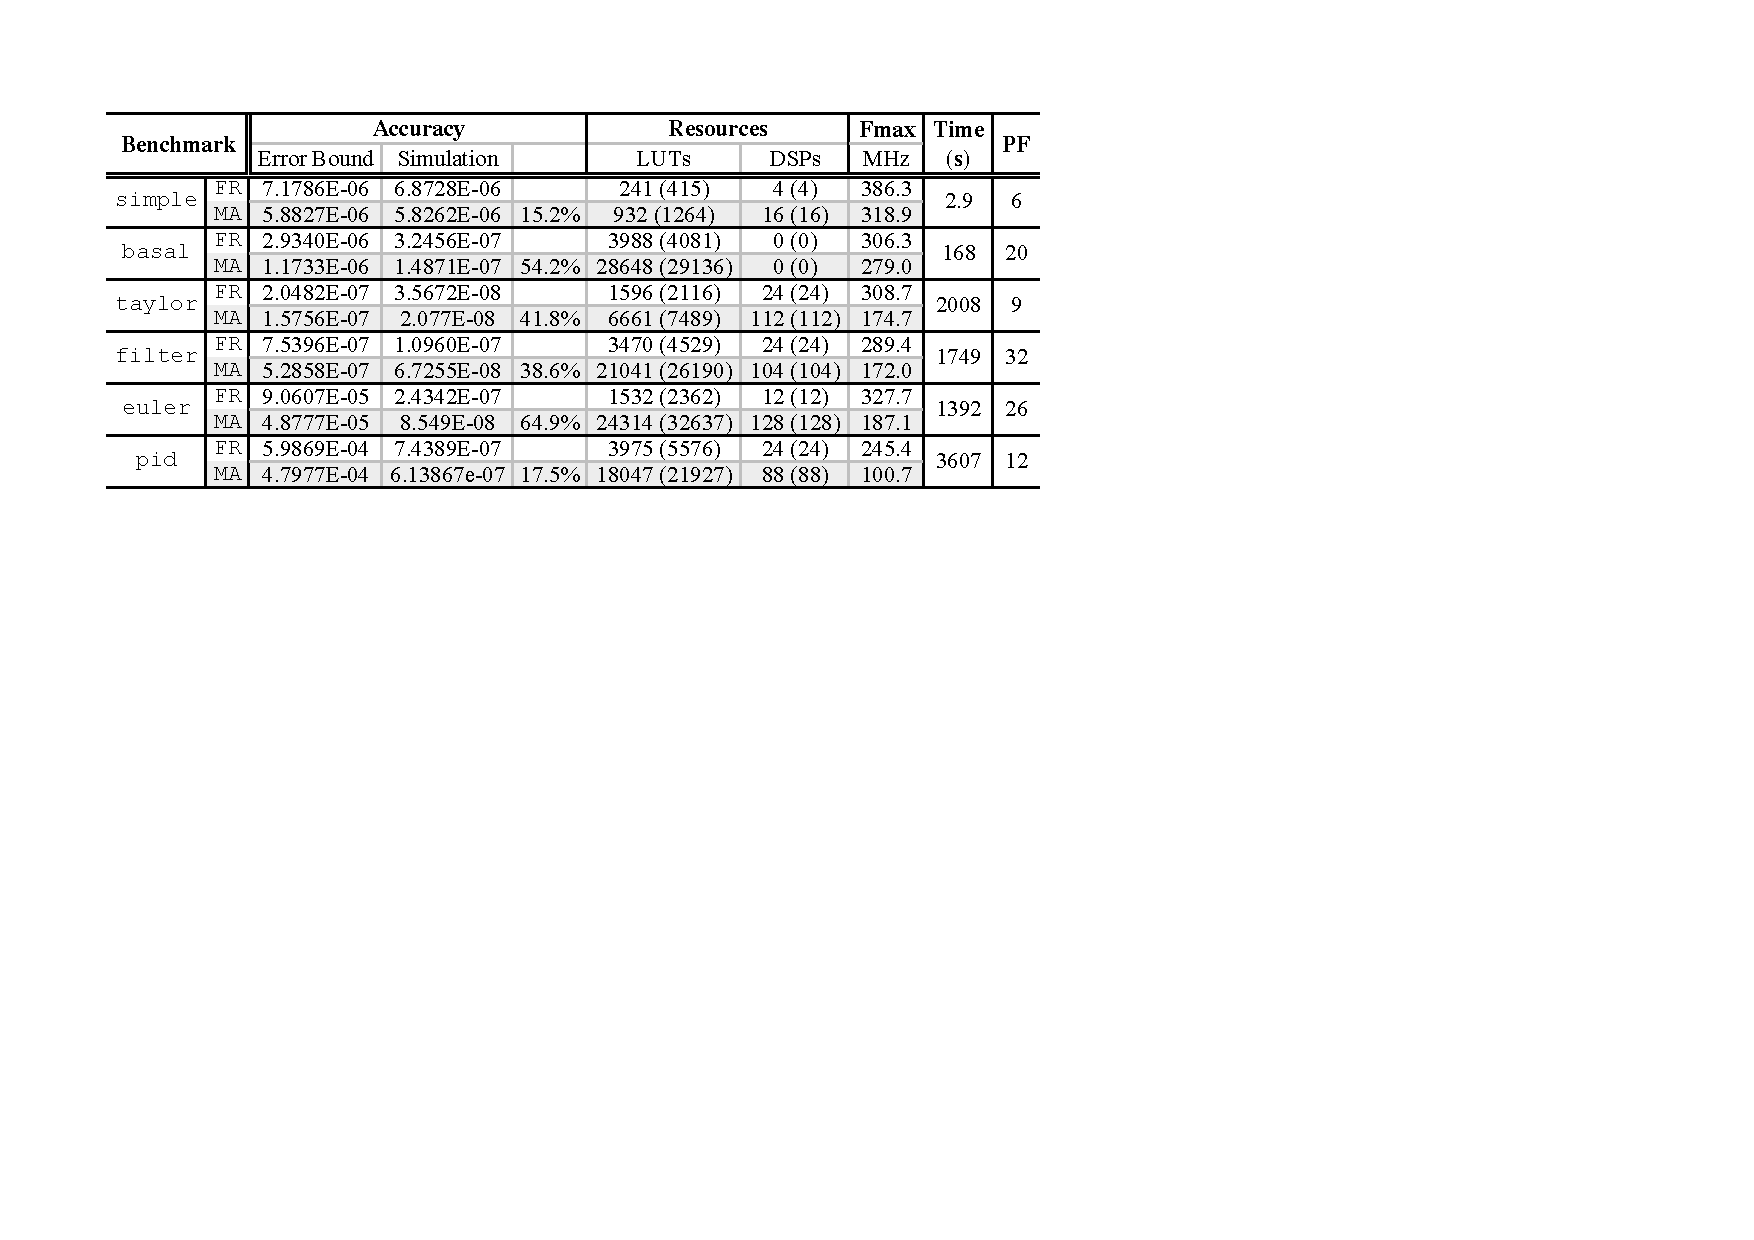
\includegraphics[width=\linewidth]{results}
    \captionof{figure}{%
    Table of optimization results.}\label{fig:results}
\end{figure}
\begin{figure}[ht]
    \centering
    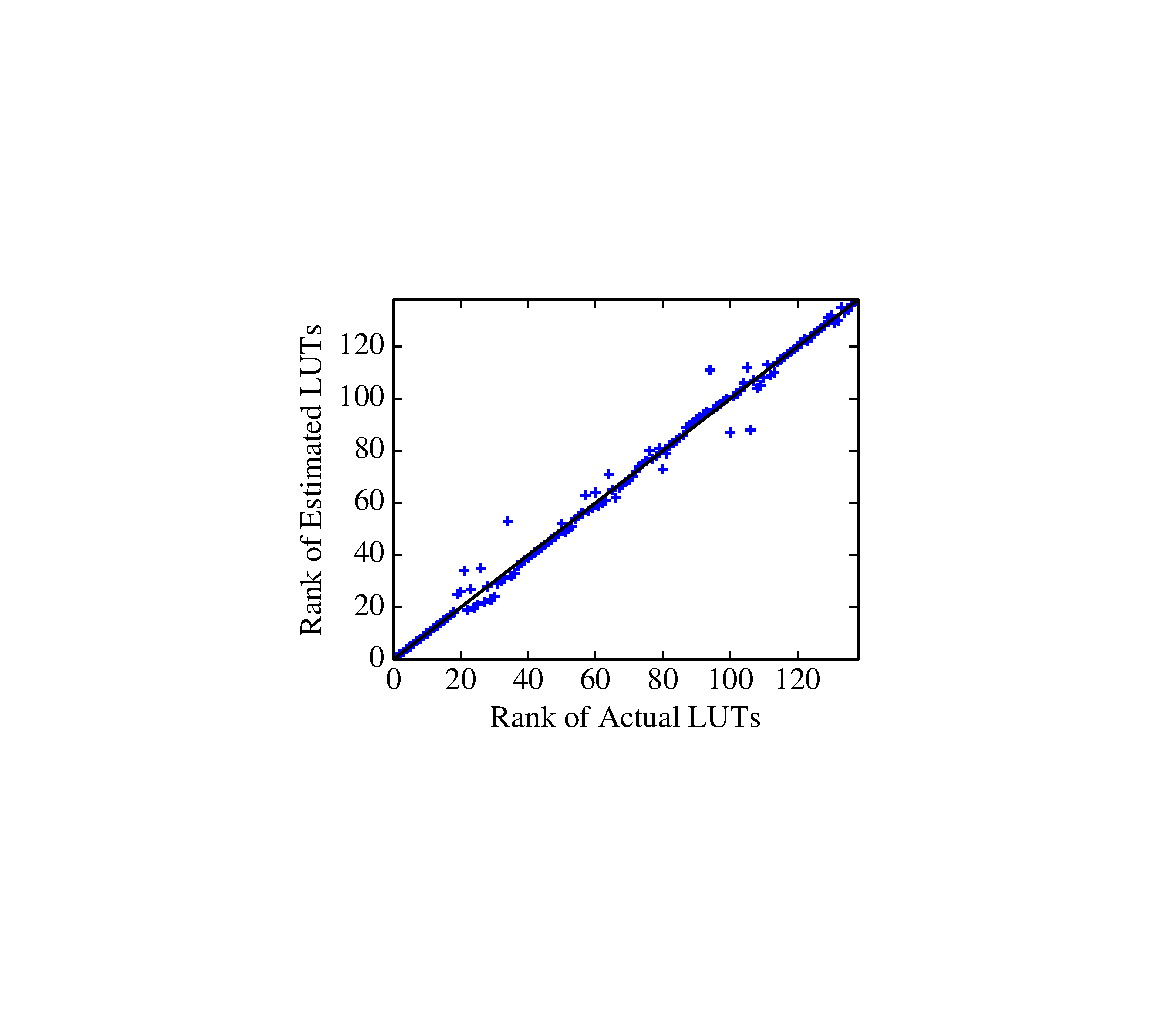
\includegraphics[scale=0.7]{rank}
    \captionof{figure}{%
    \mbox{The quality of resource estimation.}}\label{fig:rank}
\end{figure}

\begin{figure*}[ht]
    \centering
    \begin{minipage}{0.6\textwidth}
    \end{minipage}\quad\begin{minipage}{0.35\textwidth}
    \end{minipage}
\end{figure*}

The ``Resources'' columns show our estimation of the number of LUTs and
DSPs required for each of these programs, and the numbers in brackets are
the corresponding statistics obtained from Quartus synthesis.  Because
implementations on the Pareto frontier is only sensitive to how their LUTs
compare against each other, \ie~the rank, the Pareto frontier will not be
affected unless the rank is changed.  To ensure that the resource estimation
method used in our optimization can identify accurately whether an actual
implementations is on the Pareto frontier, we gathered 150 implementations
discovered across the benchmark examples, and for each one we rank its
number of estimated LUTs among them, and do the same for actual LUTs.
Figure~\ref{fig:rank} plots the rank of estimated LUTs against the rank of
actual LUTs, which shows the Pareto frontier we produced is very close to using
Quartus to count resources.

Because our benchmark examples are designed to be resource efficient, there
is no room for resource usage optimization of the original program.  However
we are able to consistently reduce the resource usage of a plain partial
loop unrolling by more than 25\%, because our optimization can discover
subexpression sharing opportunities, propagate constants values, and also
aggressively reduce the size of expressions by powerful reduction rules such as
$a - a = 0$ and $0 \times a = 0$.

Besides the choices of implementations that are either most accurate or most
resource efficient, each optimization also offers a wide selection of optimized
programs on the Pareto frontier.  For instance, Figure~\ref{fig:euler} shows
the Pareto frontier of \texttt{euler}, which has 26 different trade-off
options.  Furthermore, in the optimization of \texttt{euler}, our optimization
not only identifies that it is resource efficient when the two return variables
are computed by the same loop, but also by individually optimizing the
accuracy of the two variables, we produce a program with two loops, each with
a different goal, that is to compute their respective return variables as
accurately as possible, this generated a program that consists of two loops
that have completely different structures.  With this, we further widen the
trade-off curve with the most accurate option improving the accuracy by 65\%.
In Figure~\ref{fig:filter}, because the loop kernel of \texttt{filter} has the
expression $\sum_{i=0}^2{(a_i y_i + b_i x_i)}$, which has a large number of
equivalent expressions, without increasing the resource usage, our optimization
improves its accuracy by 14.5\%.  Because our Pareto frontier has three
dimensions, which are respectively accuracy, LUT utilization and the number of
DSPs, points within the shaded region optimize DSP count.

\begin{figure}[ht]
    \centering
    \subfloat[\texttt{euler}]{%
        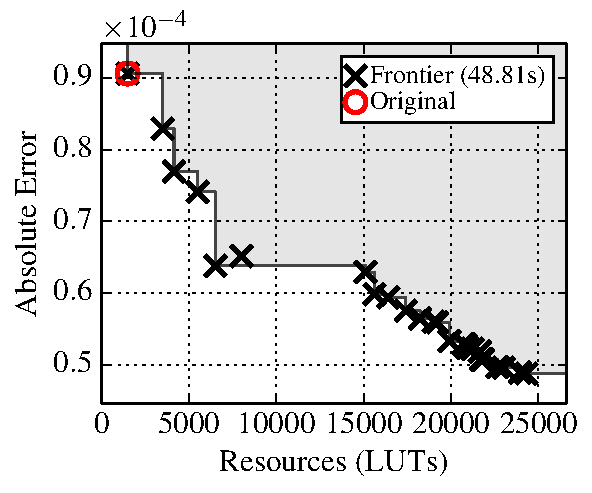
\includegraphics[width=0.6\linewidth]{euler}
        {}\label{fig:euler}
    } \\
    \subfloat[\texttt{filter}]{%
        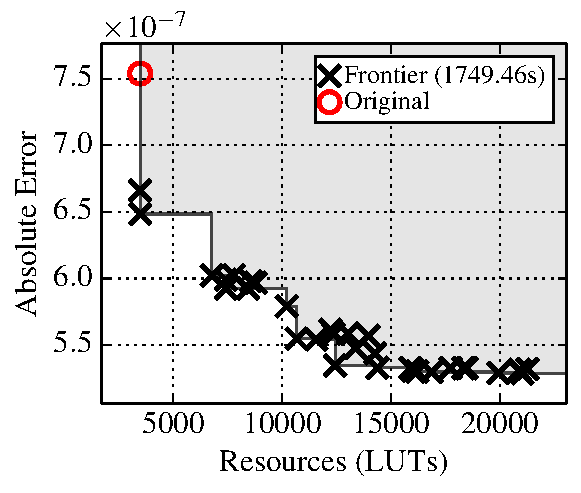
\includegraphics[width=0.6\linewidth]{filter}
        {}\label{fig:filter}
    }
    \caption{The Pareto frontier.}
\end{figure}

\section{Summary}
\label{so:sec:conclusion}

We provide a formal approach to the optimization of arithmetic expressions
for both accuracy and resource usage in high-level synthesis.  The method
proposed in this chapter and the associated tool, \soap, encompass three kind
of semantics that describe the accumulated roundoff errors, count operators in
expressions considering common subexpression elimination, and derive equivalent
expressions.  For a set of input expressions, the proposed approach works out
the respective sets of equivalent expressions in a hierarchical bottom-up
fashion, with a windowing depth limit and Pareto selection to help reduce the
complexity of equivalent expression discovery.  Using \soap, we improve either
the accuracy of our sample expressions or the resource utilization by up to
60\%, over the originals under single precision. \soap~enables a high-level
synthesis tool to optimize the structure as well as the precision of arithmetic
expressions, then to automatically choose an implementation that satisfies
accuracy and resource usage constraints.

Because we underpin our approach in formal semantics, it provides the
necessary foundation which permits us to extend the method for general
numerical program transformation in high-level synthesis.  Therefore in
Chapter~\ref{chp:progopt}, we base ourselves on the methodologies developed
in this chapter, and propose a structural approach to program optimization by
safely rewriting equivalent structures in numerical programs.



\chapter{Accurate and Resource Efficient Pipelining of Numerical Programs}
\label{chp:latopt}

\section{Introduction}

Our previous chapter introduced a new methodology to efficiently restructure
arithmetic expressions for the optimized trade-off between two performance
metrics, \ie~numerical accuracy when evaluated and area usage in synthesized
FPGA implementations.  However, this method has a substantial limitation when
applied to general numerical programs, that is, it can only be applied to
straight-line codes without control structures such as branches and loops.

The structural optimization of general numerical programs is much more complex
than that of arithmetic expressions.  The reasons are two-fold.  First,
during program execution, variables are often updated with new values.  Our
optimization should therefore perform static analysis on the values of
variables, and use the result to optimize specifically for the trade-off
between accuracy and resource usage.  Second, it is much more difficult to
formally define program equivalence, and subsequently, to search efficiently
for optimized equivalent programs.  For instance, even without the introduction
of branches and loops, the following two programs are equivalent, but
syntactically, they are very different.  In practice, it is desirable to
eliminate as much as possible the need for these syntactic rewrites that do not
affect our performance metrics.

\begin{figure}[ht]
    \centering
    \subfloat[$P_1$]{%
        \shortstack[l]{%
            \texttt{x = x + 1;} \\
            \texttt{y = 2 * x;} \\
            \texttt{x = x + 3;}
        }
    } \qquad \qquad
    \subfloat[$P_2$]{%
        \shortstack[l]{%
            \texttt{y = x + 1;} \\
            \texttt{x = y;} \\
            \texttt{y = y * 2;} \\
            \texttt{x = x + 3;}
        }
    }
    \caption{Two programs that are equivalent but syntactically different.}
    \label{fig:equiv_progs}
\end{figure}

Therefore, in this chapter, we provide answers to these two above issues.  In
the meantime, we propose a new general \emph{program} optimization technique
for numerical algorithms, which allows \texttt{if} statements as well as
\texttt{while} loops, and developed its accompanied tool, \newsoap, to enable
the joint optimization of accuracy and resource usage, as well as the trade-off
between these performance metrics.  We develop a tool, which we call \newsoap,
to perform source-to-source optimization of numerical programs targeting FPGAs,
and generate implementations that trade off resource usage and numerical
accuracy.

% floating-point arithmetic has round-off errors, exploit equivalence

Similar to the approach we have proposed in Chapter~\ref{chp:stropt}, we
exploit equivalence rules such as such as \emph{associativity} $(a + b) +
c \equiv a + (b + c)$, and \emph{distributivity} $(a + b) \times c \equiv
a \times c + b \times c$ to automatically optimize implementations for
the optimal trade-off between resource usage, \ie~the number of LUTs and
DSP elements utilized, and accuracy when evaluated using floating-point
computations.  For example, with single precision floating-point format, our
tool found that give an input $x \in [0, 100]$ and $y \in [0, 2]$, then the
program:
\begin{lstlisting}
    if (x < 1) {
        x = (x + y) + 0.1;
    } else {
        x = x + (y + 0.1);
    }
\end{lstlisting}
is most accurate when rewritten in the following form:
\begin{lstlisting}
    if (x < 1) {
        x = (x + 0.1) + y;
    } else {
        x = x + (y + 0.1);
    }
\end{lstlisting}
On the other hand, the original program uses fewest resources when
subexpressions are shared and the \iflit~statement is eliminated:
\begin{lstlisting}
    x = x + (y + 0.1);
\end{lstlisting}

This kind of optimization generates a Pareto optimal set of implementations,
which trades off accuracy and area.  A na{\"\i}ve strategy to search for
the Pareto optimal implementations is to discover all possible equivalent
expressions.  However, this would result in combinatorial explosion and become
intractable even for very small expressions~\cite{ioualalen,mouilleron}.  To
remedy this, in Chapter~\ref{chp:stropt} we proposed a novel approach, known
as \soap, to significantly reduce the space and time complexity to produce a
subset of the Pareto frontier.

% program transformation why?

Our program optimization flow is \emph{safe}, \emph{semantics-directed} and
\emph{flexible}. \emph{Safety} means that because we make use of formal
mathematics to optimize programs, our approach can be proved correct, in
the sense that when executed using exact real arithmetic, the transformed
version produces exactly the same output values as the original program.
\emph{Semantics-directed} transformation means that not only do we use
program syntax, but also the semantics to guide optimization and guarantee
safety properties of the optimized program.  Our technique obtains when
necessary, by analyzing the program, a bound and a round-off error bound on
each variable in every program location.  These information are then used
to guide program optimization.  By analyzing and manipulating not only the
syntax, but also the semantics of programs.  The meaning of a \emph{flexible}
program transformation is three-fold.  First, arithmetic computations can be
optimized across assignments, \iflit~statements and \whilelit~loops.  Secondly,
we automatically explore the numerical implications of partial loop unrolling
and loop splitting, which can create more opportunity for minimizing round-off
errors, hence further increases range of options in the Pareto frontier of
trade-offs.  Finally, our method naturally subsumes constant propagation,
redundant code elimination, and also branch and loop fusions.

% Our tool fits in the familiar setting of the high-level synthesis tool flow, as a front-end that performs the source-to-source optimization of

Our main contributions in this chapter are as follows:
\begin{enumerate}
    \vspace{-6pt}
    \item
        A new intermediate representation of the behaviour of numerical
        programs, its structure is designed to be manipulated and analyzed
        with ease.  A new framework of numerical program transformations is
        developed to enable the back and forth translation between the program
        and a new intermediate representation (IR), which preserves the
        semantics of the original program.
    \vspace{-6pt}
    \item
        Semantics-based analyses that reason about not only the resource
        utilization (number of LUTs and DSP elements), and safe ranges of
        values and errors for programs, but also potential errors such as
        overflows and non-termination.
    \vspace{-6pt}
    \item
        A new tool, \newsoap, which trades off resource usage and accuracy
        by providing a safe, semantics-directed and flexible optimization
        targeting numerical programs for high-level synthesis.
    \vspace{-6pt}
\end{enumerate}

Section~\ref{sec:related_work} provides an overview of the existing work
related in both the software and high-level synthesis community.  We then
proceed to define our program syntax in Section~\ref{sec:syntax_definition}.
Using the syntax definition, we provide a detailed formal explanation
of our numerical program transformation, which consists of three
stages.  Section~\ref{sec:program_to_mir}, {}~\ref{sec:transformations},
{}~\ref{sec:code_generation} describe in sequence how numerical programs
can be translated into MIRs, how we infer bounds and error bounds on
variables and analyze resource usage estimates for the efficient discovery
of equivalent structures in the analyzed MIR, and finally, we explain how
a chosen MIR can be translated into an optimized numerical program.  Then
we present the optimization results in Section~\ref{sec:results} and
Section~\ref{sec:conclusion} concludes this chapter.

\section{Motivation}
\label{lo:sec:motivation}

\newcommand\barr[3]{\texttt{\underline{#1[#2][#3]}}}

Figure~\ref{lo:fig:seidel_prog} gives an implementation of the Seidel stencil
computation, extracted from PolyBench~\cite{polybench}, where initially all
values in the array \verb|A| are single-precision floating-point values between
$0$ and $1$.  It resembles the typical code frequently used in fluid dynamic
simulations for solving partial differential equations and systems of linear
equations.

\begin{figure}[ht]
\begin{lstlisting}
  #define N 1024
  for (int t = 0; t < 20; t++)
    for (int i = 1; i < N-1; i++)
      for (int j = 1; j < N-1; j++)
        $\barr{A}{i}{j}$ = 0.2 * (A[i-1][j] + $\barr{A}{i}{j-1}$ +
            A[i][j] + A[i][j+1] + A[i+1][j]);
\end{lstlisting}
    \caption{%
        An excerpt from the Seidel stencil~\cite{polybench}.  The
        inter-iteration data dependence of the innermost loop is underlined
        ($\barr{A}{i}{j}$ and $\barr{A}{i}{j-1}$).
    }\label{lo:fig:seidel_prog}
\end{figure}

We start by synthesizing this program in \gls{vhls}\@.  We enable \emph{loop
pipelining} in \gls{vhls}, which asks it to optimize the loop by overlapping
its iterations.  However, we can observe that this program has very limited
opportunity for pipelining, because each iteration \verb|j| of the innermost
loop ends by writing to \verb|A[i][j]|, and the next iteration \verb|j+1|
begins by reading from \verb|A[i][j]|; this inter-iteration dependence is
highlighted in Figure~\ref{lo:fig:seidel_prog}.  Hence, it serves as our
example to motivate a better \soap~to efficiently pipeline loops.

\Gls{vhls} generates a schedule where the depth of the loop $D$ is $49$, and
\gls{ii} as enforced by the data-dependences above is $46$.  The trip count of
the innermost loop is $N = 1022$.  The overall latency of the innermost loop is
therefore $((N-1) \times \II) + D = 47,015$ cycles.

We then enable \gls{vhls}'s \gls{eb} optimization.  When synthesized, this
optimization pass tries to reorder the sequence of additions in the loop body
into a tree structure, thus reducing the $\II$ to 28 cycles, and the depth $D$
to 42 cycles, while the trip count $N = 1022$ remains the same.  The overall
latency is now $((N-1) \times \II) + D = 28,630$ cycles.  The overall resource
usage remains roughly the same.

However, as mentioned in Section~\ref{bg:sec:discovering_equivalent_programs}
of Chapter~\ref{chp:background}, \gls{vhls}'s \gls{eb} has two shortcomings.
Firstly, it is not aware of the inter-iteration data dependence and misses the
opportunity to further pipeline this loop.  Secondly, and most importantly,
\gls{vhls} does not guarantee that this optimization will not result in
catastrophic numerical inaccuracies.

We further discovered that if the loop is partially unrolled, \gls{vhls}'s
\gls{eb} did not improve the total run time, despite using a lot more
resources.  Additionally, \gls{eb} only makes use of associativity, but
not other equivalence rules.  These limitations pose great restrictions on
\gls{vhls}'s ability to produce a significantly faster implementation.

We then use the enhanced \soap~of this chapter to automatically discover
equivalent programs from the program in Figure~\ref{lo:fig:seidel_prog}.
Because our tool explores a large number of paths that lead to a Pareto
frontier of implementations, here we illustrate one of the many paths that
could be taken by minimizing latency, while trying to optimize accuracy and
resource usage.  By using just arithmetic equivalences, our tool specifically
applies transformations to alleviate the constraints on the inter-iteration
dependence, and discovers that the innermost loop can be rewritten to minimize
latency as shown in Figure~\ref{lo:fig:seidel_prog_2}.

\begin{figure}[ht]
\begin{lstlisting}
  for (int j = 1; j < 1023; j++)
    A[i][j] = 0.2 * (A[i][j-1] +
      ((A[i][j] + A[i][j+1]) + (A[i+1][j] + A[i-1][j])));
\end{lstlisting}
    \caption{The optimized program using only arithmetic equivalences.}
    \label{lo:fig:seidel_prog_2}
\end{figure}

Although this loop still has a data dependence between consecutive iterations,
this transformation greatly reduces latency because most of the loop iterations
can now be overlapped.  We find that this simple transformation can reduce
$\II$ to 19, which speeds up the original program by 2.3$\times$, using almost
the same number of \glspl{lut} and \gls{dsp} elements as the original program.
At the same time, the sequence of additions are now reordered to minimize
round-off errors, improving the accuracy by 18\%.

Our tool also supports more complex control-flow restructuring transformations,
such as partial loop unrolling, in tandem with rules that optimize memory
accesses and arithmetic calculations.  This can further reduce the loop's
latency.  In this example, unrolling the loop by a factor of two (\ie~updating
two matrix elements on every iteration and halving the trip count) and applying
other rules, results in a program with $\II = 19, D = 152, N = 511$.  When
implemented on a device it is 4.8$\times$ faster than the original, and
almost twice as accurate, at a cost of 17\% more \glspl{lut}, as shown in
Figure~\ref{lo:fig:seidel_prog_3}.

\begin{figure}[ht]
\begin{lstlisting}
  for (int j = 1; j < 1023; j += 2) {
    float t0 = A[i][j-1], t1 = A[i][j+1];
    float t2 = (A[i][j] + t1) + (A[i+1][j] + A[i-1][j]);
    float t3 = 0.04f * t2 + 0.2f *
        ((t1 + A[i][j+2]) + (A[i+1][j+1] + A[i-1][j+1]));
    A[i][j] = 0.2f * (t0 + t2);
    A[i][j+1] = 0.04f * t0 + t3;
  }
\end{lstlisting}
    \caption{The optimized program using arithmetic equivalences in tandem with
    control-flow restructuring and memory access optimization.}
    \label{lo:fig:seidel_prog_3}
\end{figure}

Further increasing the optimization effort, which enables the loop to be
deeper partially unrolled, leads to a program that is 7$\times$ faster
than the original, but uses 2.8$\times$ \glspl{lut}.  To summarize, in
Table~\ref{lo:tab:seidel_results}, we compare \gls{vhls} with \gls{eb}, against
one of the many implementations that we have explored using our tool with
the increased optimization effort.  The three columns respectively shows the
original program with loop pipelining enabled, what \gls{vhls} can achieve
alone, and the capability of our tool.  It is important to note that the
round-off error is unknown for \gls{vhls} with \gls{eb}, because it cannot
predict the impact of its unsafe optimizations on accuracy.  We performed
place-and-route for exact statistics.

\begin{table}[ht]
    \centering
    \renewcommand\arraycolsep{1.0mm}
    \newcommand\unitk{\,\text{k}}
    \newcommand\unitm{\,\text{m}}
    \newcommand\unitmu{\,\text{\textmu}}
    \newcommand\unitM{\,\text{M}}
    \newcommand\unitG{\,\text{G}}
    \newcommand\Mid[1]{\multirow{2}*{$#1$}}
    \newcommand\Shade{\cellcolor{black!10}}
    \newcommand\name[1]{\texttt{\scriptsize #1}}
    \caption{%
        Comparison among the optimized implementations generated by
        \gls{vhls}'s expression balancing and our optimizer.  The row ``Total
        run time (s)'' indicates the wall-clock time in seconds of running the
        synthesized circuits.
    }\label{lo:tab:seidel_results}
    $\begin{array}{r||r|r|r}
        \hline
        \multicolumn{1}{c||}{} &
        \multicolumn{1}{c|}{\text{\gls{vhls}}} &
        \multicolumn{1}{c|}{\text{\gls{vhls} with \gls{eb}}} &
        \multicolumn{1}{c}{\text{\gls{vhls} with \soap}} \\

        % & &
        % \multicolumn{1}{c|}{\text{with \gls{eb}}} &
        % \multicolumn{1}{c}{\text{with our tool}} \\
        \hline\hline

        \text{Clock period (ns)} &
        2.60 & 2.65 & 2.66 \\ \hline

        \Shade \text{Inner latency (cycles)} &
        \Shade 47.0\unitk & \Shade 28.6\unitk & \Shade 6.59\unitk \\ \hline

        \text{Total run time (s)} &
        2.50\unitm & 1.56\unitm & 0.358\unitm \\ \hline

        \Shade \text{\glspl{lut}} &
        \Shade 620 & \Shade 623 & \Shade 1778 \\ \hline

        \text{\gls{dsp} elements} &
        5 & 5 & 8 \\ \hline

        \Shade \text{Round-off error} &
        \Shade 10.68\unitmu &
        \Shade \text{unknown} &
        \Shade 4.31\unitmu \\ \hline
    \end{array}$
\end{table}

\section{Syntax Definition}
\label{sec:syntax_definition}

Before we discuss program transform, we first look at the syntax definition
used to write numerical programs.  Our program transformation optimizes
\numimp{} programs.  In this section, we formally introduce \numimp, a simple
imperative language which is a subset of C that supports arithmetic and Boolean
expressions, conditional branches, as well as \texttt{while} loops.  Our
language allows numerical data types $\inttype$ and $\floattype$, respectively
stand for integer and floating-point types.

We define $\aexprset, \bexprset$ as the set of arithmetic and Boolean
expressions respectively, and $\stmtset$ denotes the set of program statements.
We then have following syntax definition for expressions and \numimp{}
programs, written in the Backus-Naur Form~\cite{knuth64}:
\newcommand{\syndef}{\ensuremath\mathbin{::=}}%
\newcommand{\synor}{\ensuremath\mathbin{\mid}}%
\begin{equation}
    \begin{aligned}
        a \syndef {} &
            n \synor
            x \synor
            a_1 \odot a_2,
        \quad b \syndef x < a, \\
        s \syndef {} &
            x~\texttt{=}~a \synor
            s_1 \semicolon s_2 \synor
            \mathtt{if}~(b)~\{ s_1 \}~\mathtt{else}~\{ s_2 \} \synor
            \whilelit~(b)~\{s\}
    \end{aligned}
    \label{eq:program_syntax}
\end{equation}
We define $\odot \in \left\{ +, -, \times, / \right\}$ to be the arithmetic
operators, $n$ is a numerical constant of type either \inttype{} or \floattype;
$x \in \varset$ is a variable; $a, a_1, a_2 \in \aexprset$ are arithmetic
expressions; $b$ ranges over Boolean expressions, $\bexprset$; and similarly,
$s, s_1, s_2 \in \stmtset$ are program statements.  In our formal definition,
for the purpose of simplicity, we restrict the Boolean expressions to those
of the form $x < a$, where $x$ is a variable and $a$ is an expression;
more complex Boolean expressions are included trivially in our actual
implementation.  Although \forlit~loop is not explicitly defined in the above
syntax definition, it can be trivially derived from a \whilelit~loop.

Furthermore, we introduce the ``\verb|#pragma| \verb|soap begin|'' and
``\verb|#pragma| \verb|soap end|'' directives to delimit the code fragment
to be optimized.  We can also use ``\verb|#pragma| \verb|soap in|'' and
``\verb|#pragma| \verb|soap out|'' to provide input ranges and to declare
output variables, respectively.

As a simple example, the program in Figure~\ref{fig:syntax_example} computes an
approximate value of ${\pi^2 a}/6$.  It has two inputs $a$, a floating point
value between 0 and 1, and $n$, an integer value between 10 and 20, which
determines the number of iterations for the loop, and a return variable $y$.

\begin{figure}[ht]
    \begin{lstlisting}
    #pragma soap in \
        float a = [0.0, 1.0], int n = [10, 20]
    #pragma soap out float y
    x = 0;
    y = 0.0;
    while (x < n) {
        x = x + 1;
        y = y + a / (x * x);
    }
    \end{lstlisting}
    \caption{A simple program written with our syntax definition.}
    \label{fig:syntax_example}
\end{figure}

Despite the simplicity of our syntax, it includes all the features of
a full programming language rather than an expression language used in
Chapter~\ref{chp:stropt}.  We will add support for arrays and matrices in
Chapter~\ref{chp:latopt}, and show that this can be added with little changes
to our method.

\section{Intermediate Representations}
\label{bg:sec:intermediate}

Intermediate representations (IRs) are data structures designed to be
independent of the machine architecture and source language.  They are often
invented with the intention to ease program analysis and optimization in mind,
by abstracting information from the original program that are irrelevant to our
objectives.  In this section, we introduce several categories of existing IRs,
and delve deeper into the advantages and disadvantages of each.

\subsection{Static Single Assignment Form and Control-Flow Graph}
\label{bg:sub:ssa_cfg}

Traditionally, \emph{static single assignment} (SSA) form~\cite{alpern88,
rau92} together with \emph{control-flow graph} (CFG) are used to represent
data- and control-flow of a program~\cite{cytron91}, because they are more
favorable program representations on which optimization passes can be
implemented, when compared to the original HLL or the output language.  SSA can
be advantageous in implementing conventional optimization techniques, \eg~code
motion~\cite{cytron86}, removing redundant computations~\cite{rosen88},
and constant propagation~\cite{cytron91}.  Because the LLVM intermediate
representation (LLVM IR)~\cite{llvm_ir} is based on SSA and CFG, and is
commonly used in many HLS tools such as LegUp~\cite{legup}, we introduce SSA
and CFG by compiling the dot-product example in Figure~\ref{bg:lst:dotprod}
into as shown in Figure~\ref{bg:lst:dotprod_ll}.
\begin{figure}[ht]
    \centering
    \begin{lstlisting}[language=LLVM]
define float @dotprod(
    float* nocapture readonly %A,
    float* nocapture readonly %B) #0
{
; <label>:0
  br label %2

; <label>:1         ; preds = %2
  ret float %8

; <label>:2         ; preds = %2, %0
  %i.02 = phi i32 [ 0, %0 ], [ %9, %2 ]
  %d.01 = phi float [ 0.000000e+00, %0 ], [ %8, %2 ]
  %3 = getelementptr inbounds float, float* %A, i32 %i.02
  %4 = load float, float* %3, align 4, !tbaa !2
  %5 = getelementptr inbounds float, float* %B, i32 %i.02
  %6 = load float, float* %5, align 4, !tbaa !2
  %7 = fmul float %4, %6
  %8 = fadd float %d.01, %7
  %9 = add nuw nsw i32 %i.02, 1
  %exitcond = icmp eq i32 %9, 1024
  br i1 %exitcond, label %1, label %2
}
    \end{lstlisting}
    \caption{%
        The compiled and optimized LLVM IR output from the dot-product example
        in Figure~\ref{bg:lst:dotprod}.
    }\label{bg:lst:dotprod_ll}
\end{figure}

The LLVM IR of our example function consists of parts that are known as
\emph{basic blocks} (BB), each BB in turn often contains a label that
uniquely identifies the BB, a list of LLVM IR statements in SSA form
without any branches, \ie~the statements are executed sequentially, and a
terminator instruction, which is typically a branch instruction that leads
the control-flow to a different BB, by referencing a BB label, or a function
return.

The LLVM framework implicitly constructs a CFG from the IR code, which is a
directed graph representing the control-flow of a program.  The vertices in
the CFG constitute BBs, while the edges indicate the control-flow directions
(\ie~branches to other BBs), often with predicate attributes to determine
whether the branch is taken.  For instance, we consider the first line of third
BB in Figure~\ref{bg:lst:dotprod_ll}:
\begin{lstlisting}[language=LLVM, basicstyle=\tt]
    ; <label>:2     ; preds = %2 %0
\end{lstlisting}\vspace{-16.5pt}
which indicates it has a label value $2$ and the control-flow coming to this
BB is from either BB2 or BB0, here we use BB$n$ as a shorthand denoting a
BB labelled $n$.  Additionally, this BB ends with the branch terminator
instruction:
\begin{lstlisting}[language=LLVM, basicstyle=\tt]
    br i1 %exitcond, label %1, label %2
\end{lstlisting}\vspace{-16.5pt}
This instruction directs the control-flow to BB1 or BB2, and the variable
\verb|%exitcond| in the terminator instruction decides which branch is taken.
Finally, the complete CFG is shown in Figure~\ref{bg:fig:dotprod_cfg}.  It is
noteworthy that BB2 has two edges that leads to either \verb|BB1| or \verb|BB2|
itself.  If \verb|%exitcond| evaluates to false (\textbf{ff}), then another
iteration of BB2 will commence, otherwise (\textbf{tt}) the exit condition is
satisfied and will lead the control-flow to \verb|BB1|.
\begin{figure}[ht]
    \centering
    \tikzstyle{block} = [
        draw, fill=white, rectangle, minimum height=2em, minimum width=3em
    ]
    \tikzstyle{tmp} = [coordinate]
    \begin{tikzpicture}
        \node [] (entry) {Entry};
        \node [block, below of=entry, node distance=4em] (bb0) {\texttt{BB0}};
        \node [block, below of=bb0, node distance=4em] (bb1) {\texttt{BB1}};
        \node [block, below of=bb1, node distance=4em] (bb2) {\texttt{BB2}};
        \node [tmp, right of=bb1, node distance=5em] (bb1tr) {};
        \node [tmp, left of=bb2, node distance=8em] (bb2tl) {};
        \node [tmp, right of=bb2, node distance=8em] (bb2tr) {};
        \node [below of=bb2, node distance=4em] (exit) {Exit};
        \draw [->] (entry) -- (bb0);
        \draw [- ] (bb0)    to[out=0, in=90]    (bb1tr);
        \draw [->] (bb1tr)  to[out=-90, in=0]   (bb2);
        \draw [- ] (bb1)    to[out=180, in=90]  (bb2tl);
        \draw [->] (bb2tl)  to[out=-90, in=180] (exit);
        \draw [->] (bb2) -- node[auto, swap]{\textbf{tt}} (bb1);
        \draw [->] (bb2) to[out=-150, in=150, loop]
            node[auto, swap]{\textbf{ff}} (bb2);
    \end{tikzpicture}
    \caption{The CFG of the LLVM IR code in Figure~\ref{bg:lst:dotprod_ll}.
    }\label{bg:fig:dotprod_cfg}
\end{figure}

Each BB contains sequential computations that are represented by SSA
instructions.  The SSA form describes the operations in the original
program, such that each variable in it is assigned exactly one value.

The sequence of instructions that assigns to \verb|%3|-\verb|%9| in
Figure~\ref{bg:lst:dotprod_ll} carries out most of the computations in the
program.  It starts by reading \verb|A[i]| and \verb|B[i]|, multiplying them
together, then add the result with \verb|d| to form a new variable, and
finally, the iteration value is accumulated by $1$.  It may seem unusual that
both the accumulated sum of products and the iteration value are not assigned
to \verb|d| and \verb|i| respectively.  We can imagine two BBs, one initializes
\verb|d| and \verb|i| to zeros, the other accumulates these two variables in
a loop.  As all variables must be assigned once only, one of the BBs should
use different names for these two variables.  When the control-flow of these
two BBs join, we must introduce a way to read from the variables that are
assigned in the two BBs in the succeeding BB\@.  A new instruction, called the
$\phi$-function is therefore defined for our purpose.  The $\phi$-function
accepts two variable names as its inputs, and produce the value of either
variable as its output, determined by which preceding BB the control-flow came
from.  For example, in LLVM IR, the instruction:
\begin{lstlisting}[language=LLVM, basicstyle=\tt]
    %d.01 = phi float [ 0.000000e+00, %0 ], [ %8, %2 ]
\end{lstlisting}\vspace{-16.5pt}
shows that if the control-flow originated from BB0, then a constant zero is
returned, otherwise the control-flow had to come from BB2 and the value of
\verb|%8| is used instead.

The rationale of SSA is that we can abstract away anti- and output dependences
by never assigning to the same variable twice, while only true data-flow
dependences remain.  Anti-dependence is a dependence relation when a read
operation must precede a write to the same variable, and output dependence is
when two writes refer to the same location.  By removing these dependences
and deferring the analysis of them, certain program optimization analyses
can run much more efficiently.  Analyses that may benefit from this include
scheduling~\cite{rau94}, and liveness analysis (figure out the life time
of variables to reduce register requirements)~\cite{cytron91}, detecting
opportunities of parallelism~\cite{cytron87}, and finding equivalent parts in
the program~\cite{alpern88}.

In a cyclic CFG, the control-flow could potentially revisit a BB, and
instructions in this BB will inevitably assign a different value to the
same variable, which forms anti- and output dependences, which could have a
detrimental effect on efficient loop pipelining in some computing machines.  An
alternative IR, the \emph{dynamic single assignment} (DSA) form~\cite{rau92}
can therefore be used in place of the SSA to address this issue.  The DSA
defines a linear sequence of virtual registers for each variable, such that
every time the variable is assigned in a dynamic execution path, a new virtual
register is used.

\subsubsection{Alternatives to SSA and CFG}

There are a number of alternative IRs that are similar in construction to
the SSA and CFG approach in LLVM IR\@.  For instance, the data-dependence
graph~\cite{rau94} introduced in Section~\ref{bg:sub:sdc} are designed
for the purpose of capturing data-flow dependences in polyhedral methods.
\emph{Data-flow graph} (DFG) is a popular alternative to SSA, which is often
a directed acyclic graph (DAG) that do not contain cyclic paths.  In general,
a DFG's vertices are input, output and operation nodes, and the edges capture
the dependences between these nodes.  Both of them, however, generally do
not preserve enough information for us to reconstruct a program from the
graph itself.  A group of data structures, known as \emph{control/data flow
graphs} (CDFGs)~\cite{orailoglu86}, is commonly used to represent programs in
HLS tools, \eg~SPARK~\cite{gupta04}.  A CDFG resembles a CFG such as the one
used in LLVM IR, but in lieu of using sequential instructions in SSA form in
graph vertices, each vertex contains a \emph{data-flow graph} (DFG), where no
SSA temporary variables are used and data-flow dependences can by explicitly
identified by edges.


\subsection{Equality Saturation}
\label{bg:sub:equality_saturation}

The IRs we discussed above are all used to analyze and transform the underlying
program structure, so as to produce a new representation of the optimized
program.  In a conventional optimizing compiler, program optimization is
often carried out in a sequence of transformation passes, where each pass
accepts a program, often written in a certain IR, and produces an optimized
program in the IR\@.  The traditional practice is to always apply these
optimization phases in a fixed order, but a good ordering of these phases
is crucial to achieve a good optimized result, and the optimal ordering
varies across applications being compiled~\cite{almagor04}.  The process of
finding the optimal ordering is known as the \emph{phase-ordering problem},
which is in general undecidable~\cite{touati06} and hence is a difficult
problem.  Moreover, programs running CPUs or GPUs usually care only about
their throughput, in contrast, designs on FPGAs concern us with additional
objectives besides run time, such as power consumption and resource utilization
that impact the quality of synthesized circuit.  Multiple designs that
trade-off these objectives could exist, and which design to choose relies
on the specifics of the use case.  It is therefore sensible to explore the
design space by optimizing multiple objectives simultaneously.  For the
above reasons, it is desirable to have an IR and the associated optimization
procedures to efficiently discover equivalent structures that lead to different
implementations of the original program.

In software, a novel approach called \emph{equality saturation} is proposed
in~\cite{tate09} to find multiple possible optimized variants of the original
program, and subsequently deal with the phase-ordering problem.  It creates
a new graph-based IR, \emph{program expression graph} (PEG), to encode the
effects of executing the program.

To begin, we review the structure of the PEG, by considering a simple loop
example in Figure~\ref{bg:fig:factorial}.  By understanding how the PEG can
be evaluated for the output values, we can interpret how the PEG captures the
control- and data-flow information of the program.  PEGs, similar to arithmetic
expressions expressed in a tree structure, can be evaluated in a bottom-up
fashion, by recursively propagating computed values from the leave nodes to the
root of the tree.  However, unlike arithmetic expressions which are acyclic,
edges in PEGs may form cycles to express loops in the original program.
\begin{figure}[ht]
    \newsavebox{\factlstbox}
    \begin{lrbox}{\factlstbox}
    \begin{lstlisting}
int x = 1;
int y = 1;
while (y <= 10)
{
    x = y * x;
    y = y + 1;
}
    \end{lstlisting}
    \end{lrbox}
    \centering
    \subfloat[The original program.]{%
        \begin{minipage}{0.4\textwidth}
            \usebox{\factlstbox}
        \end{minipage}\label{bg:lst:factorial_c}
    }
    \subfloat[The resulting PEG.]{%
        \begin{minipage}{0.5\textwidth}
            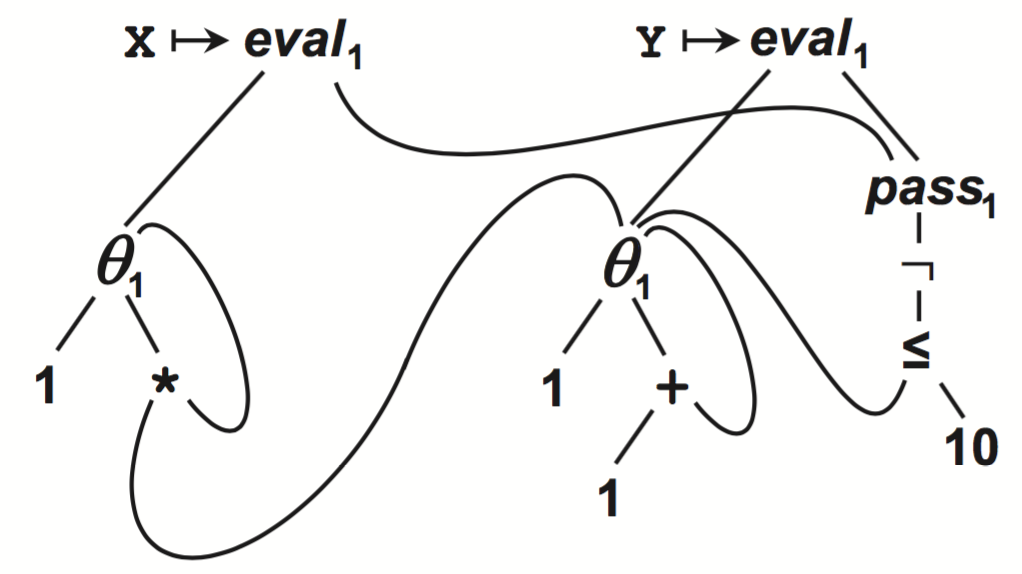
\includegraphics[width=\textwidth]{bg/fig/factorial_peg.png}
        \end{minipage}\label{bg:fig:factorial_peg}
    }
    \caption{%
        A simple loop which computes the factorial of 10, and the resulting
        PEG\@.  This example and its PEG, showing computations that lead to the
        final \texttt{x} and \texttt{y}, is taken from~\cite{tate09}.
    }\label{bg:fig:factorial}
\end{figure}

\subsubsection{Data-Flow Nodes}

All loops in the PEG are formed by $\theta$ nodes, which is used in the
following form:
\begin{center}
    \vspace{-16.5pt}
    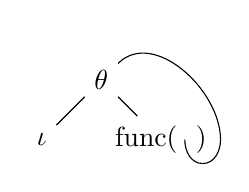
\begin{tikzpicture}
        \node (theta) at (0, 0) {$\theta$};
        \node (init) at (-5ex, -5ex) {$\iota$};
        \node (func) at (5ex, -5ex) {$\mathrm{func}(~~)$};
        \node[coordinate] (input) at (7ex, -5ex) {};
        \node[coordinate] (mid1) at (8.5ex, -7ex) {};
        \node[coordinate] (mid2) at (10ex, -5ex) {};
        \draw[-] (theta) -- (init);
        \draw[-] (theta) -- (func);
        \draw[-] (input) to[out=-90, in=180] (mid1);
        \draw[-] (mid1) to[out=0, in=-90] (mid2);
        \draw[-] (mid2) to[out=90, in=45] (theta);
    \end{tikzpicture}
    \vspace{-16.5pt}
\end{center}
where it accepts two child graphs, $\iota$ and $\mathrm{func}$, and
$\mathrm{func}$ further takes the $\theta$ node as one of its inputs to
form a complete cycle.  Evaluating a $\theta$ node produces a list of
values computed iteratively by the node's subgraph.  The first value in the
list, is the computed result of $\iota$, which we name $i$, and values in
the rest of the sequence are iteratively computed by $\mathrm{func}$.  In
functional programming, this is similar to iteratively computing the fixpoint
$\fixpoint{F}$ of an initial list $[i]$, which is defined as:
\begin{equation}
    \fixpoint{F} ([i]) = \lim_{n \to \infty} F^n ([i]),
    \quad\text{where~}
    F(v) = \mathrm{prepend}\left(
        \iota, \mathrm{map}\left( \mathrm{func}, v \right)
    \right)
\end{equation}
here, $\mathrm{map}(\mathrm{func}, v)$ applies the subgraph computation
$\mathrm{func}$ to all elements in the list $v$, and $\mathrm{prepend}(\iota,
v^\prime)$ prepends the element $\iota$ to the list $v^\prime$.

For example, the following subgraph in Figure~\ref{bg:fig:factorial_peg}
evaluates to the sequence $[1, 2, 3, 4, \mathellipsis]$:
\begin{center}
    \vspace{-16.5pt}
    \begin{tikzpicture}
        \node (theta) at (0, 0) {$\theta_1$};
        \node (init) at (-5ex, -5ex) {$1$};
        \node (add) at (5ex, -5ex) {$+$};
        \node (one) at (0, -10ex) {$1$};
        \node[coordinate] (mid) at (8ex, -5ex) {};
        \draw[-] (theta) -- (init);
        \draw[-] (theta) -- (add);
        \draw[-] (add) -- (one);
        \draw[-] (add) to[out=-45, in=-90] (mid);
        \draw[-] (mid) to[out=90, in=45] (theta);
    \end{tikzpicture}
    \vspace{-16.5pt}
\end{center}

It is noteworthy that $\theta$ nodes may have subscripts.  For instance,
in Figure~\ref{bg:fig:factorial_peg}, both nodes $\theta_1$ share the same
subscript $1$.  This is used to indicate that the two sequences produced
by both $\theta$ nodes iterate simultaneously, \ie~they share the same
iteration count so that a new value for \verb|x| can be computed as we update
\verb|y|.  Therefore, the $\theta_1$ node in the left of this figure produces
a sequence of the factorials of $[1, 2, 3, \mathellipsis]$, \ie~$[1, 2, 6, 24,
\mathellipsis]$.

Computation nodes, such as arithmetic $+$ and boolean operators $\leq$ and
$\neg$ in Figure~\ref{bg:fig:factorial_peg}, operates on a list of values, by
performing the computation on each value in the list.

For instance, the $\leq$ node accepts two inputs, the sequence $[1, 2, 3,
\mathellipsis]$ derived earlier, and a scalar $10$, computes the result of $x
\leq 10$ for each element $x$ in the sequence, and finally produces the list,
where $\truelit$ and $\falselit$ respectively denote true and false boolean
values:
\begin{equation}
    [
        \truelit, \truelit, \truelit, \truelit, \truelit,
        \truelit, \truelit, \truelit, \truelit, \truelit,
        \falselit, \falselit, \falselit, \mathellipsis
    ].
\end{equation}
The subsequent $\neg$ node then negates all elements in the list:
\begin{equation}
    [
        \falselit, \falselit, \falselit, \falselit, \falselit,
        \falselit, \falselit, \falselit, \falselit, \falselit,
        \truelit, \truelit, \truelit, \mathellipsis
    ].
    \label{bg:eq:bool_seq}
\end{equation}

\subsubsection{Control-Flow Nodes}

The $\theta$ node encodes an infinite sequence of computed values, whereas
the output value of the program is a scalar.  By further representing
control-flow information in PEG, it becomes possible to refer to a
single value in this sequence, as the output of the program.  To do so,
Tate~\etal~\cite{tate09} further introduce $\mathrm{pass}$ and $\mathrm{eval}$
nodes.  The $\mathrm{pass}$ node finds the first true ($\truelit$) value
in a sequence of boolean values, and returns the index of this value, and
$\mathrm{eval}$ takes two child nodes, where the first node evaluates to a list
$v$ of values, and the second is an scalar $n$ used to select a scalar value
from $l$, as the output of this node.

To illustrate, the $\mathrm{pass}_1$ node finds the first $\truelit$ in the
list~\eqref{bg:eq:bool_seq}, $11$.  The $\mathrm{eval}$ node of the output
variable \verb|y| subsequently fetches the $11$-th item from the list $[1, 2,
3, 4, \mathellipsis]$ we produced earlier, which is $11$.  Similarly we can
apply the same process to find that the output \verb|x| is $10!\,$, \ie~the
factorial of 10.

By using $\mathrm{pass}$ and $\mathrm{eval}$ nodes to represent the
control-flow in an algebraic fashion, and mixing data- and control-flows
together in the graphical representation, PEGs provide us with greater
opportunities to optimize data-flow across control-flow boundaries and vice
versa.  Simple equivalence rules can be defined for these nodes algebraically.
For instance, arithmetic operators can be distributed over $\theta$ and
$\mathrm{eval}$, \eg~$\mathrm{eval}(j, k) + i \equiv \mathrm{eval}(j + i, k)$.
Complex transformations can therefore be deductively constructed from these
simple equivalence rules.

\subsubsection{Equivalence Finding}

By applying transformation passes to the PEG, their approach detects the
incremental modifications, and append these changes to the original PEG\@.  The
new changes, represented as extra structures in the PEG, are linked to their
corresponding equivalent nodes by equivalence edges.  These edges indicate a
pair of subgraphs are equivalent, forming a PEG with equivalent structures,
or named E-PEG, that could capture multiple PEGs in the same structure.  The
resulting E-PEG is similar to the one in Figure~\ref{bg:fig:epeg}, where dashed
edges indicate equivalences.  It is notable that each edge allows a binary
choice, therefore the number of PEGs can be represented in an E-PEG could be
exponential in the number of equivalence edges.
\begin{figure}[ht]
    \centering
    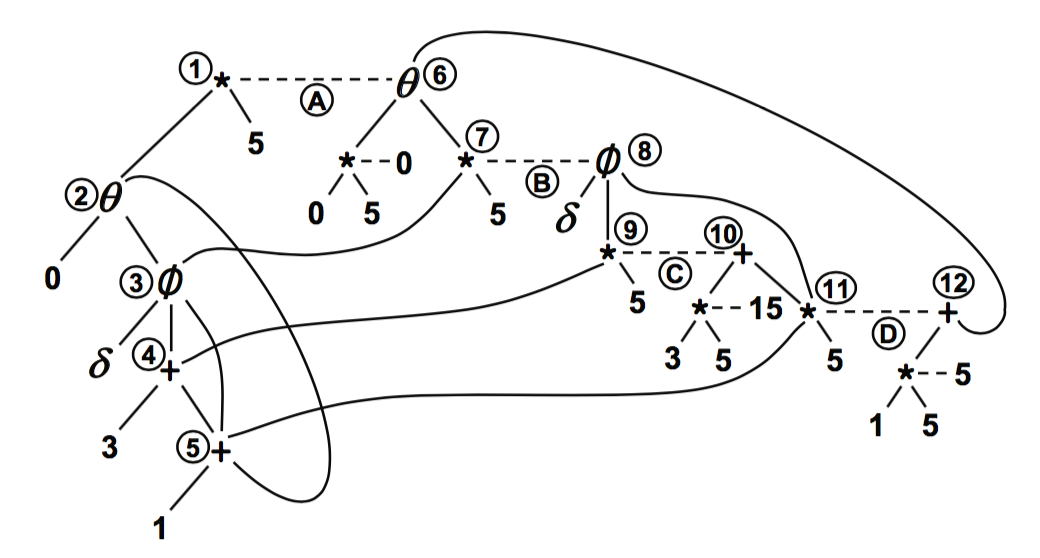
\includegraphics[width=0.8\linewidth]{bg/fig/epeg.png}
    \caption{An simple E-PEG example, taken from~\cite{tate09}.
    }\label{bg:fig:epeg}
\end{figure}

By repeatedly applying all possible passes to the E-PEG, this graph will
eventually saturate, \ie~no more equivalent structure can be added to the graph
because all possible equivalences are now discovered.  This process and the
resulting E-PEG is more space-time efficient than enumerating all possible PEGs
along the path, because E-PEG encourages sharing common subgraphs, even across
equivalent edges.  This saturated graph can always be produced regardless of in
what order we apply the passes, hence preventing the phase-ordering problem.
Furthermore, E-PEG defers the decision of whether an optimization should be
committed until we have reached full saturation, allowing the global optima to
be discovered.  In contrast, because each optimization pass in a conventional
compiler is performed once, the compilers must make the decision to commit
changes immediately after applying the optimization, which consequently often
results in local optima.

\section{Structural Optimization}
\label{lo:sec:structural_optimization}

From a numerical program, we can generate an MIR using the translation in
Section~\ref{lo:sec:intermediate}.  The next step is to transform the MIR, and
discover MIRs that are equivalent to the original MIR in real arithmetic, but
may execute differently in finite-precision arithmetic because of round-off
errors.

\subsection{Algorithm}
\label{lo:sub:algorithm}

% Our optimization starts by partitioning the MIR into sub-MIRs.  This further
% reduces the size of the search space, \ie~equivalent MIRs reachable using our
% transformation rules.  This speeds up the rest of the optimization process,
% because these rules are not applied on partition boundaries.

As discussed in Section~\ref{lo:sec:introduction}, even a small expression
could have a huge number of equivalent ones.  Exhaustively discovering all
equivalent MIRs would result in combinatorial explosion of the number of
equivalent MIRs in the search space.  For this reason, we base ourselves on an
algorithm from \SOAP{} that search efficiently, by discovering equivalences
in a bottom-up hierarchy.  In this section we discuss the improvements we
have made to the algorithm which further increases the performance of this
algorithm.

Our first contribution is that instead of optimizing the MIR immediately, we
start by partitioning the MIR into multiple smaller sub-MIRs.  In turn, each
are optimized separately and generate a set of equivalent sub-MIRs.  We then
select combinations from these sub-MIRs to be merged, this generates a set of
MIRs that are equivalent to the original.  Finally, we preserve those MIRs
merged on the Pareto frontier.

Figure~\ref{lo:alg:optimize} shows the pseudocode of the optimization
algorithm, it takes as an input an MIR graph, and produces a set of equivalent
graphs that are estimated to be Pareto-optimal when converted into C programs
and synthesized into circuits.  Although this algorithm deals with a special
case, \ie~a root node $op$ with two child subtrees $e_1, e_2$, it can
easily be generalized to an arbitrary number of child subtrees.  Here, $e
\stackrel{r}{\rightsquigarrow} e'$ means $e^\prime$ can be obtained by
transforming part of the graph $e$ in accordance with the transformation rule
$r$.  The next section discusses the transformation rules we used.

The algorithm starts by discovering equivalences in the leaves of an MIR,
and progress upwards for equivalent structures of the individual components
that make up the graph, until the roots of the graph, where we have a set of
equivalent MIRs to the original MIR\@.  As it traverses through the MIR, the
algorithm calculates the performance metrics at each node, using the analyses
presented in the next section.  Transformations that are not Pareto-optimal are
immediately pruned from the search space, thus reducing the average complexity
of the algorithm.

Our second contribution is the \textsc{Prune} function.  We rely on this
function to efficiently steer the direction of our Pareto frontier as we
discover new candidates.  It takes as an input the set of equivalent MIRs
that we have discovered, and prune MIRs in this set to reduce its size, this
keeps the size of discovered MIRs tractable.  The \SOAP{} framework prunes the
MIRs that are Pareto-suboptimal, leaving only those that are on the Pareto
frontier.  However, because our Pareto frontier is three-dimensional, there is
a large increase in the number of Pareto-optimal MIRs.  This Pareto pruning
approach is no longer feasible for our benchmark examples.  To tackle this,
we introduce another step in \textsc{Prune} to further decrease the number of
MIRs in the set by sampling.  We developed a new sampling algorithm, inspired
by Poisson-disk sampling algorithm~\cite{bridson07}, which samples the Pareto
frontier by first randomly selecting one point, then iteratively grows the set
of points by adding the neighbours from the point that are separated by at
lease a certain distance, we search by bisection for the distance that keeps
20\% of all point in the Pareto frontier.  This method is superior to random
sampling, because random sampling often samples points that are close together,
which usually are very similar implementations.

We found that with our improvements, the algorithm is significantly faster than
the original optimization algorithm in \SOAP, with a 5-fold increase in speed,
at a cost of less points on the Pareto frontier.

\begin{figure}[ht]
    \centering
    \begin{algorithmic}
\Function{Optimize}{$op(e_1, e_2)$}
    \State{$s_1 \gets$ \Call{Optimize}{$e_1$}}
    \State{$s_2 \gets$ \Call{Optimize}{$e_2$}}
    \State{$s^\prime \gets \varnothing$}
    \State{%
        $s \gets \left\{
            op(e^\prime_1, e^\prime_2) \mid
            e^\prime_1 \in s_1 \wedge e^\prime_2 \in s_2
        \right\}$}
    \While{$s \neq s^\prime$}
        \State{$s^\prime \gets s$}
        \State{$s^{\prime\prime} \gets \varnothing$}
        \For{$r \in \mathrm{transformation\_rules}, e \in s$}
            \For{%
                $e^\prime \text{~where~}
                    e \stackrel{r}{\rightsquigarrow} e^\prime$
            }
                \State{%
                    $s^{\prime\prime} \gets
                        s^{\prime\prime} \cup \left\{ e^\prime \right\}$}
            \EndFor
        \EndFor
        \State{$s \gets$ \Call{Prune}{$s^{\prime\prime}$}}
    \EndWhile
    \State{\Return{$s$}}
\EndFunction
    \end{algorithmic}
    \caption{%
        The algorithm we used for the efficient discovery of equivalent
        structures in MIRs.
    }
    \label{lo:alg:optimize}
\end{figure}

\subsection{Transformation Rules}
\label{lo:sub:transformation_rules}

This section details the transformation rules used in our structural
optimization algorithm in Figure~\ref{lo:alg:optimize}.  These transformation
rules, each on its own is not revolutionary, but for the first time, we bring
them together to show a much better automatic structural optimization on the
latency, resource usage and accuracy of numerical programs, than using only a
subset of them.

\begin{table}[t]
\newcommand\tstack[1]{\begin{tabular}[t]{@{}l@{}}#1\end{tabular}}
    \centering
\begin{tabular}{@{}l@{~~~}l@{}}
\hline
\multicolumn{2}{c}{\bf Arithmetic Rules}
\\\hline
\emph{Associativity} & \texttt{(a + b) + c} $~\rightsquigarrow~$ {\tt a + (b +
c)}
\\\hline
\emph{Commutativity} & \texttt{a + b} $~\rightsquigarrow~$ \texttt{b + a}
\\\hline
\emph{Distributivity} & \texttt{(a + b) * c} $~\rightsquigarrow~$ \texttt{a * c + b * c}
\\\hline
\emph{Negation} & \texttt{a - b} $~\rightsquigarrow~$ \texttt{a + (-b)}
\\\hline
\emph{Subtraction} & \texttt{(a + b) - (a + b)} $~\rightsquigarrow~$ \texttt{0}
\\\hline
\emph{Const.\ prop.} & \texttt{(a * b + c / d) * 0} $~\rightsquigarrow~$ \texttt{0}
\\\hline
\emph{Division} & \texttt{a / (5 / b)} $~\rightsquigarrow~$ \texttt{a * b * 0.2}
\\\hline\hline
\multicolumn{2}{c}{\bf Control Flow Restructuring Rules}
\\\hline
\emph{Partial loop unrolling} & \tstack{\texttt{for(i=0;i<1000;i++)\string{C\textsubscript{i};\string}} $~\rightsquigarrow~$ \\ \texttt{for(i=0;i<1000;i+=2)\string{C\textsubscript{i}; C\textsubscript{i+1};\string}}}
\\\hline\hline
\multicolumn{2}{c}{\bf Access Reduction Rules}
\\\hline
\emph{Multiple reads} & \texttt{x=A[i-{}-]; y=A[i+1];} $~\rightsquigarrow~$ \texttt{x=A[i-{}-]; y=x;}
\\\hline
\emph{Multiple writes} & \texttt{A[i++]=x; A[i-1]=y;} $~\rightsquigarrow~$ \texttt{A[i++]=y;}
\\\hline
\emph{Read after write} & \texttt{A[i++]=x; y=A[i-1];} $~\rightsquigarrow~$ \texttt{A[i++]=x; y=x;}
\\\hline
\emph{Indep.\ accesses} (where $\texttt{i}\not\equiv\texttt{j}$) & \texttt{A[i]=x; y=A[j];} $~\rightsquigarrow~$ \texttt{y=A[j]; A[i]=x;}
\\\hline
\end{tabular}
\caption{%
    Before-and-after examples to demonstrate the transformation rules
    we used. The arithmetic and control flow rules are inherited from
    Chapter~\ref{chp:progopt}; the access reduction rules are introduced in
    this work.}\label{lo:tab:rules}
\end{table}

\SOAP{} provides a range of equivalence rules that are used in the
optimization, such as associativity, distributivity, commutativity, constant
propagation, and partial loop unrolling.  In Table~\ref{lo:tab:rules}, we list
those rules that proved effective when minimizing loop latencies.  Although
these rules are used to transform MIRs, we present before-and-after examples
written in C to allow the effect of each rule to be readily understand.

Our new rules, the access reduction rules, with formal definitions below and
examples in Table~\ref{lo:tab:rules}, remove extraneous data dependences that
arise after partial unrolling.  These rules, along with partial loop unrolling,
mostly do not really impact latency, because they are very well studied in
polyhedral compilation, and tools such as Vivado HLS can make use of them
automatically.  However, they give the necessary freedom to arithmetic rules
to affect latency.  The rules are as follows, where $A$ is an array, $\bar{i},
\bar{j}$ are subscripts, and $e, e^\prime$ are expressions:
\begin{itemize}

    \item \emph{Multiple reads}, eliminates the second of two reads of the same
    location.  It arises naturally from the MIR, as common subexpressions are
    shared.

    \item \emph{Multiple writes}, eliminates a write that is overwritten:
    \begin{equation}
        \update{\update{A}{\bar{i}}{e}}{\bar{i}}{e^\prime}
            \rightsquigarrow \update{A}{\bar{i}}{e^\prime}
    \end{equation}

    \item \emph{Read after write}, eliminates a read from a location
    that has just been written:
    \begin{equation}
        \access{\update{A}{\bar{i}}{e}}{\bar{i}} \rightsquigarrow e
    \end{equation}

    \item \emph{Independent accesses}, allows two array operations to be
    reordered if it can be proved that they never access the same location:
    \begin{equation}
        \access{\update{A}{\bar{i}}{e}}{\bar{j}}
            \rightsquigarrow \access{A}{\bar{j}},
        \text{if~} \bar{i} \not\equiv \bar{j}
    \end{equation}
    We visualize this rule also in the following sample MIR transformation:
    \begin{equation}
        \label{lo:eq:indep_reads_mir}
        \begin{tikzpicture}[mir]
            \node[mirnode] (var_y) at (0,0) {\texttt{y}};
            \node[mirnode] (access)[right=of var_y] {$\accessop$};
            \node[mirnode] (j1)    [below right=of access, xshift=-2mm] {\texttt{j}};
            \node[mirnode] (update)[below left=of access, xshift=6mm] {$\updateop$};
            \node[mirnode] (var_A) [left=of update] {\texttt{A}};
            \node[mirnode] (a2)    [below left=of update] {\texttt{A}};
            \node[mirnode] (i2)    [below=of update] {\texttt{i}};
            \node[mirnode] (x2)    [below right=of update] {\texttt{x}};

            \draw[|->] (var_y) -- (access);
            \draw[|->] (var_A) -- (update);
            \draw[<-] (access) -- (j1);
            \draw[<-] (access) -- (update);
            \draw[<-] (update) -- (x2);
            \draw[<-] (update) -- (i2);
            \draw[<-] (update) -- (a2);
            \brackets{(current bounding box)}
        \end{tikzpicture}
        \rightsquigarrow
        \begin{tikzpicture}[mir]
            \node[mirnode] (var_y) at (0,0) {\texttt{y}};
            \node[mirnode] (access)[right=of var_y] {$\accessop$};
            \node[mirnode] (j1)    [below right=of access, xshift=-2mm] {\texttt{j}};
            \node[mirnode] (update)[below left=of access] {$\updateop$};
            \node[mirnode] (var_A) [left=of update] {\texttt{A}};
            \node[mirnode] (a2)    [below left=of update] {\texttt{A}};
            \node[mirnode] (i2)    [below=of update] {\texttt{i}};
            \node[mirnode] (x2)    [below right=of update] {\texttt{x}};

            \draw[|->] (var_y) -- (access);
            \draw[|->] (var_A) -- (update);
            \draw[<-] (access) -- (j1);
            \draw[<-] (access) to[bend left=20] (a2);
            \draw[<-] (update) -- (x2);
            \draw[<-] (update) -- (i2);
            \draw[<-] (update) -- (a2);
            \brackets{(current bounding box)}
        \end{tikzpicture}
    \end{equation}

\end{itemize}

These rules may not seem powerful on their own, but when combined with other
structural rules, they enable our tool to detect dependences that can be
removed in the MIR\@.  This could in turn allow more opportunities for the
rules to further reduce loop latency.  By way of illustration, we optimize the
following program for latency, which computes a Fibonacci series generalized to
real numbers:
\begin{lstlisting}
    for (int i = 2; i < 1023; i++)
        A[i] = A[i - 1] + A[i - 2];
\end{lstlisting}
If we simply partially unroll this loop, we can see that because of the
rigid array access pattern, associativity cannot be applied easily to the
loop kernel.
\begin{lstlisting}
    for (int i = 2; i < 1023; i++) {
        A[i] = A[i - 1] + A[i - 2];
        A[i + 1] = A[i] + A[i - 1];
    }
\end{lstlisting}
By applying the above access reduction rules first, we give associativity the
freedom to reduces latency by half and improves accuracy by 50\%:
\begin{lstlisting}
    for (int i = 2; i < 1023; i += 2) {
        float t1 = A[i - 1], t2 = A[i - 2];
        A[i] = t1 + t2;
        A[i + 1] = 2 * t1 + t2;
    }
\end{lstlisting}
Therefore, without the above access reduction rules, it is not possible to
reach this optimized implementation.  Conversely, it is not possible to relax
scheduling constraints due to inter-iteration dependences without arithmetic
equivalence rules, as these reduction rules are there to assist transformation
rules that could really make a difference in latency.  Therefore all these
rules in Table~\ref{lo:tab:rules} are essential to the optimization of latency
in numerical programs.

\section{Performance Analysis}
\label{lo:sec:performance_analysis}

This section explains how we analyze \glspl{mir} for our three performance
metrics: latency, resource usage, and accuracy.

\subsection{Latency Analysis}
\label{lo:sub:latency}

The purpose of our latency analysis is not to create a complete scheduling
of numerical programs, as this would be computationally expensive, and would
need to be repeated for tens of thousands of equivalent programs.  Instead, it
computes a lower bound of the loop's \gls{ii}, the \acrfull{mii}.  (Recall that
the initiation interval is the number of clock cycles that must elapse between
the starts of two consecutive loop iterations, and is determined by data
dependences and resource constraints.)  We then compute the overall latency of
the loop, and subsequently, the total latency of the program.

Following LegUp~\cite{legup}, we compute \gls{mii} values using the first
few steps of modulo \gls{sdc} scheduling~\cite{canis14} introduced in depth
in Section~\ref{bg:sub:sdc} of Chapter~\ref{chp:background}, by viewing
\glspl{mir} as dependence graphs, as the structure of \glspl{mir} already
captures intra-iteration data-dependences.  In addition to this, we add extra
latency information as attributes on the edges of \glspl{mir}, plus new edges
to form cycles that capture inter-iteration data-dependences.  The analysis is
carried out in three stages.

The analysis starts with the \gls{mir} of the loop under analysis. Each edge
in the \gls{mir}, say $s\rightarrow t$, represents a data-dependence: the
operation at node $s$ must be evaluated fully before the operation at $t$
can begin.  The first step is to add a pair $\pair{l}{d}$ for each edge of
the \gls{mir}\@.  Here, $l$ is the \emph{latency} of the edge (the number of
\emph{clock cycles} that must elapse between the start of $s$ and the start
of $t$) and $d$ is the \emph{dependence distance} (the number of \emph{loop
iterations} that must elapse between the start of $s$ and the start of $t$).
Because all operations in the \gls{mir} are performed in a single iteration,
all edges have $d=0$.  The value of $l$ is given by the latency of the
operation at node $s$; if $s$ corresponds to an input variable or a numerical
constant, then $l=0$.

The second stage is to add edges to form a cyclic dependence graph that
captures \gls{raw} dependences across loop iterations.  This step involves
checking whether each pair of ``$\accessop$'' and ``$\updateop$'' nodes
has a dependence, and if so, adding a new edge between them with latency
and dependence distance attributes.  As an example, consider the \gls{mir}
in~\eqref{lo:eq:array_example} and assume each iteration increments \verb|i|
by 1.  Because in the original program, \verb|A[i]| and \verb|A[i+1]| are
respectively reading from and writing to the same array \verb|A|, we need to
check if these accesses could touch the same memory location in different
iterations.  For this, our analysis formulates an \gls{ilp} problem for
the dependence distance, and solves it using the \gls{isl}~\cite{isl}.
In this example, the dependence distance is 1 because the value written
to \verb|A[i+1]| in the current iteration \verb|i| is immediately used
in the next iteration \verb|i+1|.  Similarly, we also add new edges
for reads and writes to the same variable, which can be treated as a
special array with only one element. Our analysis yields the \gls{mir} in
Figure~\ref{lo:fig:example_latency}.

\begin{figure}[ht]
    \centering
    \begin{tikzpicture}[mir, node distance=8mm, inner sep=0]
        \node[mirnode] (A) at (0,0) {\texttt{A}};
        \node[mirnode, inner sep=1.5mm] (update) [right=of A] {$\updateop$};
        \node[mirnode] (A1)    [below left=of update] {\texttt{A}};
        \node[mirnode] (plus)  [below=of update] {$+$};
        \node[mirnode] (i1)    [below left=of plus] {\texttt{i}};
        \node[mirnode] (n1)    [below right=of plus] {$1$};
        \node[mirnode] (times) [below right=of update, xshift=11mm] {$\times$};
        \node[mirnode] (n2)    [below left=of times] {$2$};
        \node[mirnode] (access)[below right=of times] {$\accessop$};
        \node[mirnode] (A2)    [below left=of access] {\texttt{A}};
        \node[mirnode] (i2)    [below right=of access] {\texttt{i}};

        \draw[|->] (A) -- (update);
        \draw[<-] (update) to[auto, swap, pos=0.8] node{\smallpair00} (A1);
        \draw[<-] (update) to[auto] node{\smallpair{10}0} (plus);
        \draw[<-] (update) to[auto] node{\smallpair70} (times);
        \draw[<-] (plus) to[auto, swap] node{\smallpair00} (i1);
        \draw[<-] (plus) to[auto] node{\smallpair00} (n1);
        \draw[<-] (times) to[auto, swap] node{\smallpair00} (n2);
        \draw[<-] (times) to[auto] node{\smallpair20} (access);
        \draw[<-] (access) to[auto, swap] node{\smallpair00} (A2);
        \draw[<-] (access) to[auto] node{\smallpair00} (i2);
        \brackets{(current bounding box)}
\begin{pgfinterruptboundingbox}
        \draw[<-,dashed] (access) to[auto, swap, pos=0.2, out=45, in=30]
        node{\smallpair{-2}1} (update);
\end{pgfinterruptboundingbox}
    \end{tikzpicture}
    \caption{%
        The \acrshort{mir} with edges labelled with latency attributes.
    }\label{lo:fig:example_latency}
\end{figure}

Note the new dashed edge from the $\updateop$ node to the $\accessop$ node,
which is labeled $\pair{-2}{1}$.  The first value, $-2$, signifies that the
latency of the edge between $\times$ and $\accessop$, which is 2 cycles, is
canceled out because the multiplier can reuse its output from the previous
iteration as the input for the current iteration. The second value, $1$,
indicates that there is a data flow dependence from iteration $i$ to iteration
$i+1$.

We assume no limit on the number of operators we can allocate, so operators
do not constraint \gls{ii}.  However, in \gls{vhls}, each array is usually
translated into a dual-port \gls{ram}, which allows only two accesses per
clock cycle~\cite{vivado_hls}, and thus constraints \gls{mii}.  Following
Section~\ref{bg:sub:sdc}, we evaluate:
\begin{equation}
    \ResMII = \max_{a\,\in\,A} \left\lceil \frac{n_a}{r_a} \right\rceil,
\end{equation}
where $a \in A$ ranges over all arrays in the loop body, $n_a$ is the number of
accesses to the array $a$, \ie~the number of shared $\accessop$ and $\updateop$
nodes accessing the array $a$ in the dependence graph, and $r_a = 2$ is the
maximum number of accesses allowed per cycle per array.

The final step is to calculate \acrfull{recmii} which is defined in
Section~\ref{bg:sub:sdc} as:
\begin{equation}
    \RecMII = \max_{c\,\in\,C} \left\lceil \frac{l_c}{d_c} \right\rceil,
\end{equation}
where $c \in C$ ranges over all cycles in the graph, and $l_c$ and $d_c$ are
respectively the sums of all latencies and dependence distances of the edges in
the cycle.  Because a typical \gls{mir} with array accesses could have a very
large number of cycles, we efficiently search for an \gls{mii} using a modified
Floyd--Warshall algorithm~\cite{floyd62}, following~\cite{rau94}.

Finally, we estimate the total latency $L$ of the loop with:
\begin{equation}
    L = (N - 1) \MII + D,
    \text{~where~}
        \MII = \max\left(\RecMII, \ResMII\right).
    \nonumber
\end{equation}
Recalling from Section~\ref{bg:sub:sdc} in Chapter~\ref{chp:background}, $N$ is
the maximum \emph{trip count}, \ie~the loop's total number of iterations, and
$D$ is the loop's depth, \ie~the total number of cycles per iteration.

Because we optimize \glspl{mir} in a bottom-up hierarchy, when an
expression that does not constitute a inter-iteration dependence is
optimized, its latency is estimated by scheduling its operations by using
an \gls{alap}~\cite{wang_hls} scheduling algorithm, where each operation
is scheduled to the latest opportunity, while respecting the order of data
dependences.

Because the expression is eventually used in a loop, and the \gls{ii} of
the loop is critical to how fast the loop can execute, it is necessary
to start optimizing for \gls{ii} as soon as possible.  Therefore, in our
latency analysis of a \gls{mir} or an expression that is a fragment of a
inter-iteration dependence cycle, our algorithm automatically shortens any
paths between any pairs of dependent accesses in the \gls{mir}\@, as we use the
latency analysis as a component to manoeuvre our optimization on the Pareto
frontier.  Moreover, we place greater weights on dependent accesses with
smaller dependence distances, because these impact the resulting loop \gls{ii}
more significantly than larger distances.  For instance, consider a loop body
that has two dependent accesses across iterations, \ie~the graph contains two
cycles:
\begin{lstlisting}
    A[i] = $f\left( \texttt{A[i-1]},\,\texttt{A[i-2]} \right)$;
\end{lstlisting}
Here as we optimize this program in a bottom-up hierarchy, $f$ is optimized
before the loop body.  For \gls{mii} considerations, the subexpression tree $f$
is thus rewritten such that the following latency cost is minimized:
\begin{equation}
    L = \max \left(
        \frac{l_1}{d_1}, \frac{l_2}{d_2}
    \right).
\end{equation}
Here, $l_1$ and $l_2$ are respectively the lengths
of the longest latency-weighted paths from the nodes
$\access{\texttt{A}}{\overline{\texttt{i}-1}}$ and
$\access{\texttt{A}}{\overline{\texttt{i}-2}}$ to the root of $f$, and $d_1$
and $d_2$ are respectively the dependence distances of the two nodes to the
write of \verb|A|, where $d_1 = 1$ and $d_2 = 2$.


\subsection{Resource Utilization Analysis}
\label{lo:sub:resource}

The hardware resource usage analysis of Chapter~\ref{chp:stropt} captures the
sharing of common subexpressions, but cannot analyze resource binding, which
allows common operations to be shared across clock cycles. For instance, in the
floating-point expression $\vara + (\varb + \varc)$, the two additions can be
computed using one addition operator only.  In this section, we develop a new
resource usage analysis that fully understands how resources are shared in an
\gls{fpga} implementation of numerical programs.

We rely on the foundation of resource usage analysis from
Chapters~\ref{chp:stropt} and~\ref{chp:progopt}, which counts the number
$n_\opsymbol$ of each type of operation $\opsymbol \in \opset$, while maximally
sharing common subexpressions.  In a pipelined loop, we compute a lower bound
$a_\opsymbol$ on the number of instances of $\opsymbol$ that must be allocated,
using the following formula:
\begin{equation}
    a_\opsymbol = \left\{
        \begin{aligned}
            & \left\lceil \frac{n_\opsymbol}{\MII} \right\rceil
            && \quad \text{if $\opsymbol$ is shared}, \\
            & \quad n_\opsymbol
            && \quad \text{otherwise}.
        \end{aligned}
    \right.
\end{equation}
Here, integer operators are typically not shared~\cite{cong15}, so the number
of operations is the number of allocated instances.

For instance, if we know that a pipelined loop has $\MII = 3$, and each
iteration uses 6 multiplications, then we can compute that we need to
synthesize at least 2 multipliers.

For straight-line code, non-pipelined loops, and different loops, we use a
simple \gls{alap} scheduling~\cite{wang_hls} to estimate resource utilization.

Finally, we accumulate the number of \glspl{lut} and \gls{dsp} elements
for all allocated operators.  In addition, we estimate the number of
\glspl{lut} required by multiplexers generated for sharing operators, where
$R^\mathrm{LUTs}_\mathrm{mux}$ approximates $1/n$ of the number of \glspl{lut}
required by an $n$-to-1 multiplexer.  The final result is the estimated
resource utilization for the full program:
\begin{equation}
    \begin{aligned}
        r_\mathrm{LUT} &=
            \sum_{\opsymbol \in \opset} \left(
                a_\opsymbol R^\mathrm{LUTs}_\opsymbol +
                \left( n_\opsymbol - a_\opsymbol \right)
                    R^\mathrm{LUTs}_\mathrm{mux}
            \right), \\
        r_\mathrm{DSP} &=
            \sum_{\opsymbol \in \opset} a_\opsymbol R^\mathrm{DSPs}_\opsymbol,
    \end{aligned}
\end{equation}
where $R^\mathrm{LUTs}_\opsymbol$ and $R^\mathrm{DSPs}_\opsymbol$ denote the
number of \glspl{lut} and \glspl{dsp} required by one operator $\opsymbol$
respectively.


\subsection{Accuracy Analysis}
\label{lo:sub:accuracy}

We extend the accuracy analysis of Chapter~\ref{chp:progopt} to support arrays.
Because our benchmark suite consists of programs with large arrays, we keep
the analysis efficient by treating an \emph{entire} array as a pair of a
floating-point interval and an interval of accumulated round-off errors.  These
intervals accumulate all values that are assigned to the array, and never
shrink the range bounded by these intervals when we assign new values to an
array location.  We therefore define the read and write accesses to an array as
follows in the accuracy analysis:
\begin{equation}
    \begin{aligned}
        \exprerrorfunc{\access{A}{\bar\imath}}\sigma^\sharp
        &= \exprerrorfunc{A}\sigma^\sharp, \\
        \exprerrorfunc{\update{A}{\bar\imath}{e}}\sigma^\sharp
        &= \exprerrorfunc{A}\sigma^\sharp \sqcup
           \exprerrorfunc{e}\sigma^\sharp,
    \end{aligned}
\end{equation}
where $A \in \varset$ is an array variable, $\bar\imath$ is a subscript
to index an element in $A$, $e \in \sexprset$ is an expression, and
$\sigma^\sharp \in \errordom$ is the input abstract program state (recall from
Section~\ref{po:sec:accuracy_analysis} of Chapter~\ref{chp:progopt}).

Alternatively, we can view each element $A[i]$, where $i$ is a tuple with $N$
non-negative integers, in an $N$-dimensional array $A$ as a variable.  Updating
$A$ thus produces an abstract state which collects all elements in $A$:
\begin{equation}
    \begin{aligned}
        \exprerrorfunc{\access{A}{\bar\imath}}\sigma^\sharp
        &= \bigsqcup_{i \in \exprerrorfunc{\bar\imath}\sigma^\sharp}
            \sigma^\sharp \left( A[i] \right), \\
        \exprerrorfunc{\update{A}{\bar\imath}{e}}\sigma^\sharp
        &= {\left[
            A[i] \mapsto \sigma^\sharp \left( A[i] \right) \sqcup
                \exprerrorfunc{e}\sigma^\sharp
        \right]}_{i \in \exprerrorfunc{\bar\imath}\sigma^\sharp},
    \end{aligned}
\end{equation}
where $i \in \exprerrorfunc{\bar\imath}\sigma^\sharp$ ranges over all possible
indices that are tuples with $N$ non-negative integers, where $A$ is an
$N$-dimensional array.

Additionally, because most of the loops in our benchmark programs consist
of nested loops and have large iterations, the fixpoint analysis routine
in Section~\ref{po:sub:fixpoint} is modified to analyze only a small
fraction of the innermost loop execution of a loop nest.  By ensuring the
innermost loop iterator increments by the same amount, we can guarantee the
accuracy analysis to be fair for each equivalent implementation for fixpoint
expressions with different unroll factors.  For the experimental outcomes in
Section~\ref{lo:sec:results}, we analyze $10\%$ of the total executions of an
innermost loop for the purpose of optimization.

Finally, we further use the dependence analysis in the \gls{mir} graph
explained in Section~\ref{lo:sub:latency} to detect whether errors are
accumulated across iterations.  This process is carried out by first analyzing
the \gls{mir} of the loop body for intra-iteration dependences.  The absence
of such dependences indicates the round-off errors do not accumulate across
iterations, and it suffices to analyze the fixpoint expression for one loop
iteration.

\section{Results}
\label{sec:results}

In this section we optimize a set of numerical programs using our tool in
a benchmark suite with six different examples.  We use the IEEE 754 32-bit
single precision format with rounding to nearest mode as the data types of the
floating-point values used in these examples.  The benchmark consists of two
introductory numerical programs, and four real applications that are frequently
encountered in numerical analyses, and round-off errors have big impacts on the
quality of their execution:
\begin{itemize}
    \item \texttt{simple}: for an input $x \in [0, 20]$, we repeatedly multiply
it with $0.9$, until the result is less than or equal to 1, the number of
iterations is dependent on $x$ and can only be determined by analyzing the
program.
    \item \texttt{basal}: the example in~\eqref{eq:syntax_example}.
    \item \texttt{taylor}: the Taylor expansion of $\cos(x + y)$, with single
precision inputs $x \in [-0.1, 0.1]$ and $y \in [0, 1]$, and an integer $n \in
[10, 20]$, which determines the bound on the iteration count.
    \item \texttt{filter}: computes the unit step response of a 3rd-order
infinite impulse response (IIR) filter, and all coefficients are bounded by
$[0.0, 0.2]$, and it has a fixed iteration count 20.
    \item \texttt{euler}, it uses Euler's method to solve the differential
equation of a harmonic oscillator $\ddot{x} + \omega^2 x = 0$, with both an
initial stationary position $x$ and $\omega^2$ bounded by $[0.0, 1.0]$, a step
size of $0.1$, and an iteration count $n \in [0, 20]$.  It returns the position
$x$ and velocity $\dot{x}$.
    \item \texttt{pid}, the example PID controller that was used as a case
study in~\cite{damouche14} as a motivation of automated accuracy optimization
of numerical programs, we make it more challenging by changing constant
coefficients to be bounds to model not only one, but a huge selection of PID
controllers, with $kp \in [9.0, 10.0]$, $ki \in [0.5, 0.7]$ and $kd \in [0,
3.0]$, and an iteration count $n \in [0, 20]$.
\end{itemize}

Our configuration for the efficient discovery of equivalent expressions
uses a depth limit $k = 2$, and a maximum 3 times of partial unrolling is
performed.  For each program we optimize it with our tool to discover a wide
range of implementations, and select the most accurate and least resource
demanding equivalent implementations for further analysis.  The selected
implementations are then simulated 1000 times, with a sample of 1000 unique
random inputs for each benchmark example, then we compare the maximum round-off
errors encountered.  Finally, our back-end transpiler produces C source codes
from MIRs, and they are synthesized with LegUp~\cite{legup}, an open source
HLS tool, with floating-point operator sharing turned off to achieve maximum
frequency, then compiled and verified with Quartus, targeting an Altera
Stratix IV device (EP4SGX530) for the actual resource usage statistics and the
frequency achieved.

Figure~\ref{fig:results} shows the results of optimizing the above benchmark
examples.  The rows labeled ``\texttt{FR}'' and ``\texttt{MA}'' respectively
show the statistics for the most resource efficient, and the most accurate
implementations.  ``Time (s)'' shows the time required for the optimization,
and ``PF'' shows the number of trade-off options in the Pareto frontier.  The
optimization runtime is longer than a typical compiler optimizer, because
during equivalent structure discovery, a significant amount of equivalent
structures are examined.  The values shown in the ``Error Bound'' column are
the maximum absolute errors found by our tool, while ``Simulation'' shows the
actual absolute value bound on round-off errors found during simulation, and
the percentage shows the actual accuracy improvement found in simulation of
``\texttt{MA}'' over ``\texttt{FR}''.  For each of these benchmark problems,
the optimization for accuracy of them translates well to the actual reduction
of simulated round-off errors in actual executions.  They all show improvements
in accuracy over the original by up to 65\% in actual execution.  The analyzed
round-off errors are larger than the simulated bounds, because our accuracy
analysis considers the worst case scenario, and the error bounds are computed
with the worst possible round-off error for each arithmetic computation,
whereas in actual computations worst case round-off errors are extremely rare.

\begin{figure}[ht]
    \centering
    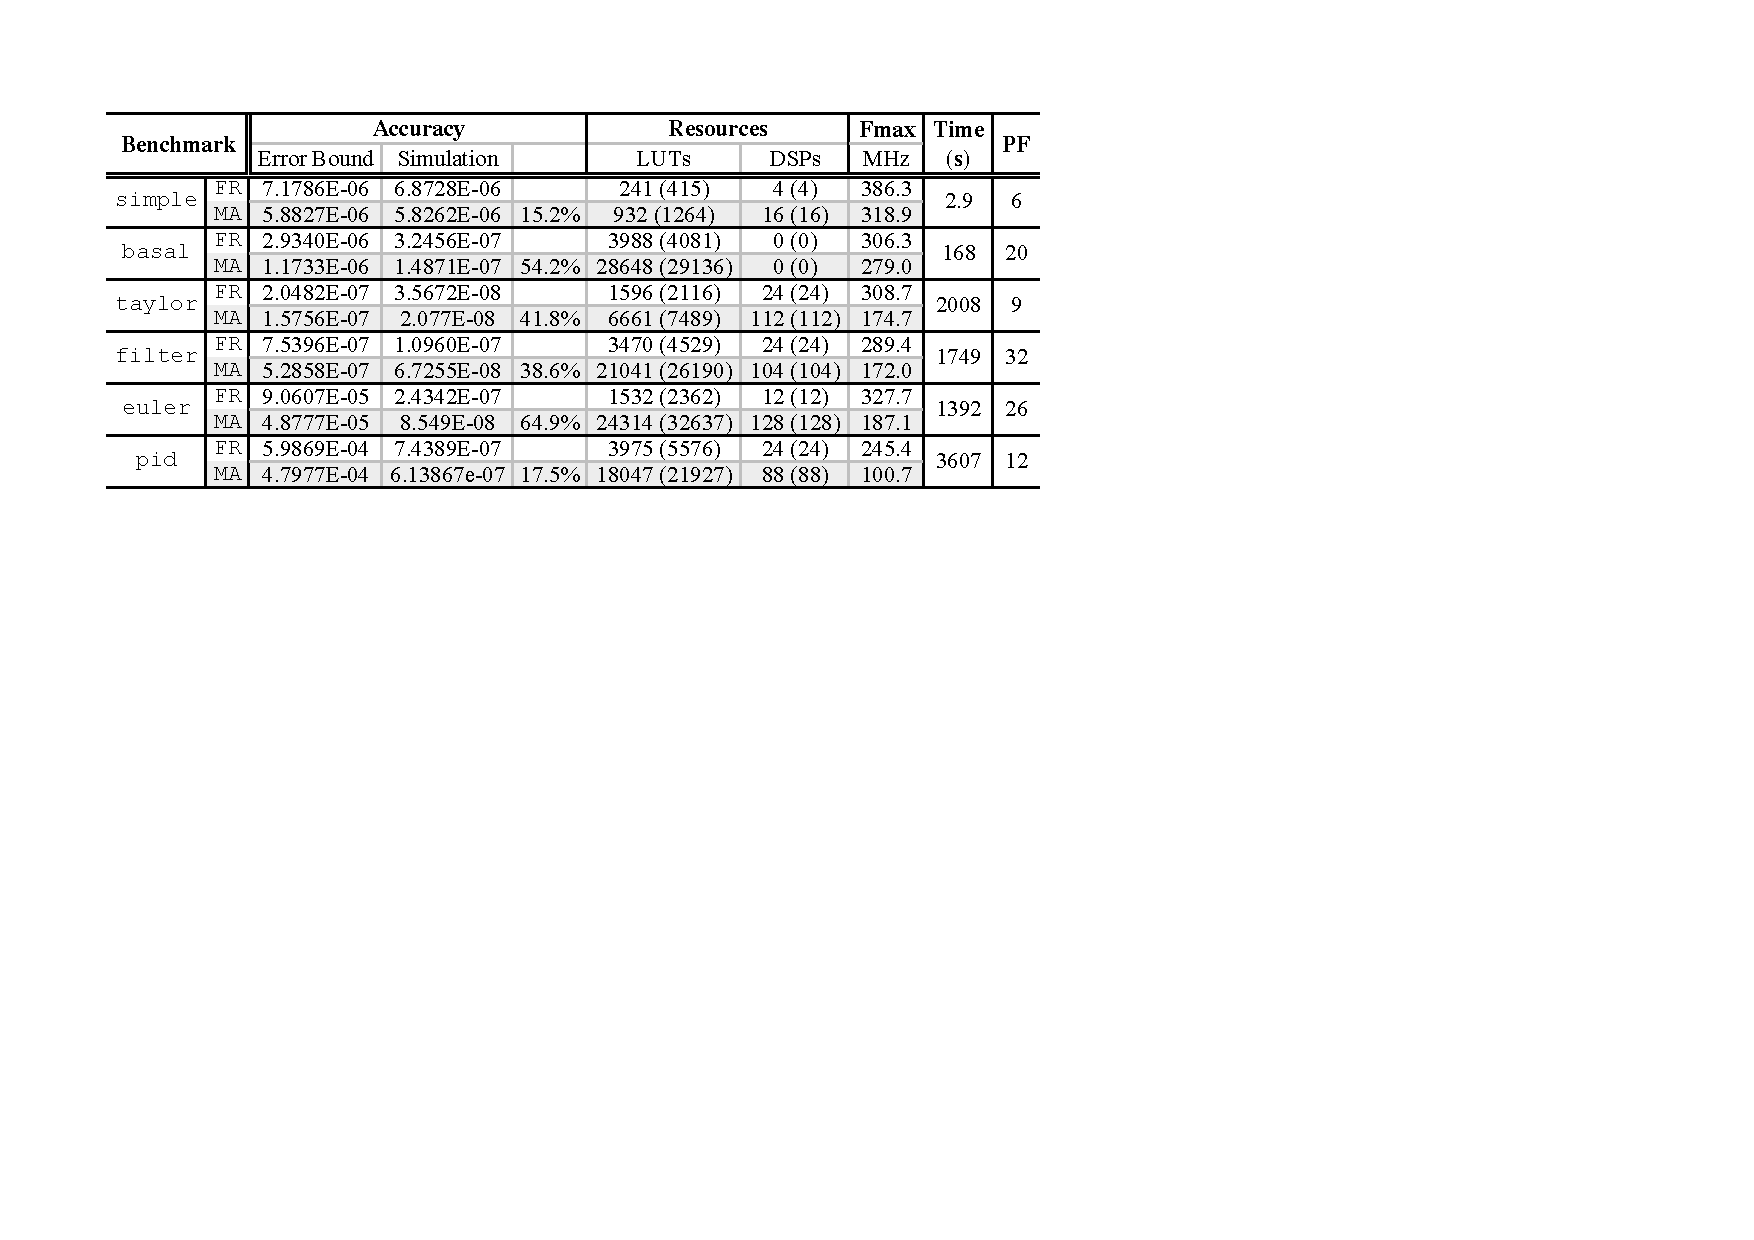
\includegraphics[width=\linewidth]{results}
    \captionof{figure}{%
    Table of optimization results.}\label{fig:results}
\end{figure}
\begin{figure}[ht]
    \centering
    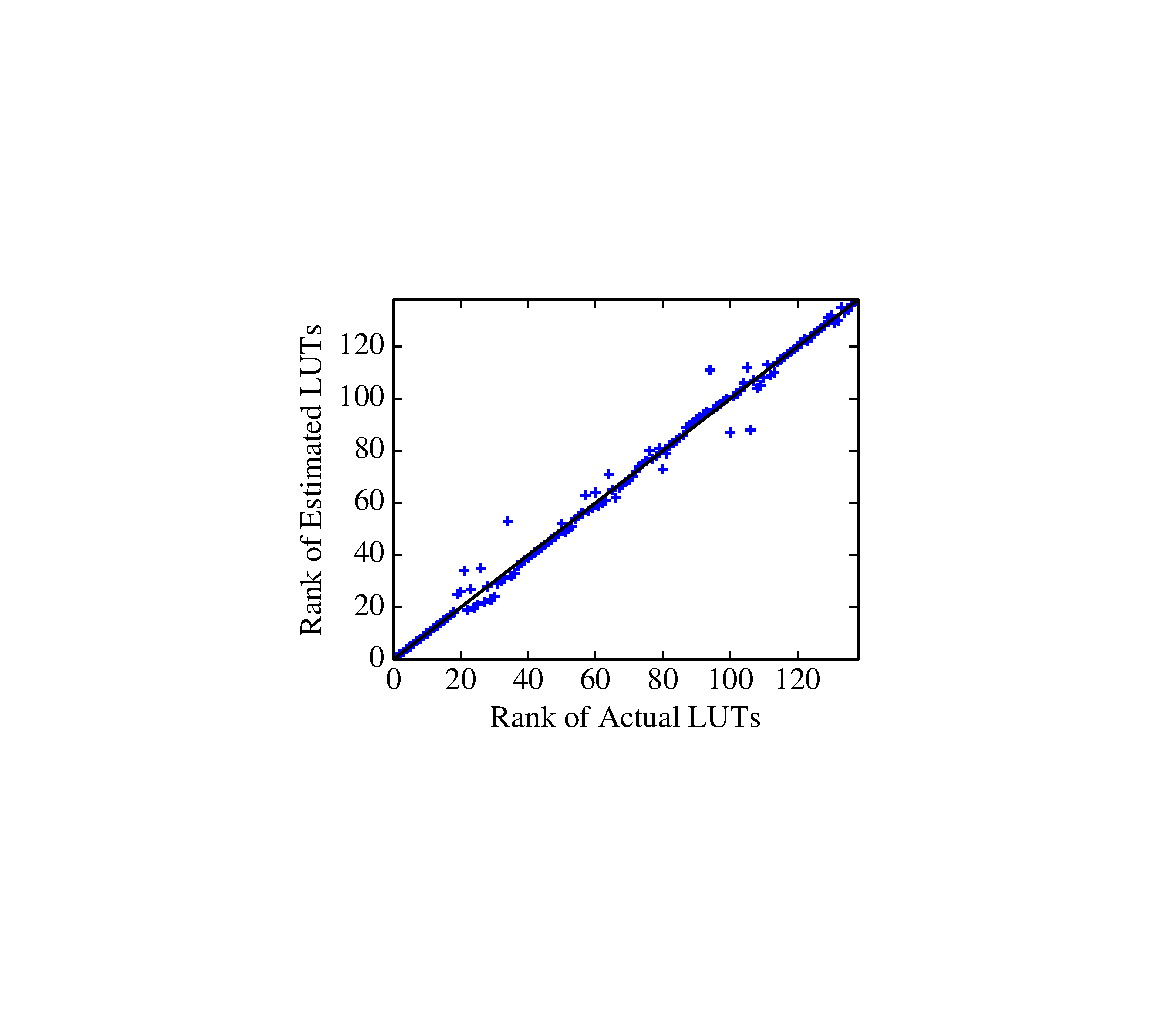
\includegraphics[scale=0.7]{rank}
    \captionof{figure}{%
    \mbox{The quality of resource estimation.}}\label{fig:rank}
\end{figure}

\begin{figure*}[ht]
    \centering
    \begin{minipage}{0.6\textwidth}
    \end{minipage}\quad\begin{minipage}{0.35\textwidth}
    \end{minipage}
\end{figure*}

The ``Resources'' columns show our estimation of the number of LUTs and
DSPs required for each of these programs, and the numbers in brackets are
the corresponding statistics obtained from Quartus synthesis.  Because
implementations on the Pareto frontier is only sensitive to how their LUTs
compare against each other, \ie~the rank, the Pareto frontier will not be
affected unless the rank is changed.  To ensure that the resource estimation
method used in our optimization can identify accurately whether an actual
implementations is on the Pareto frontier, we gathered 150 implementations
discovered across the benchmark examples, and for each one we rank its
number of estimated LUTs among them, and do the same for actual LUTs.
Figure~\ref{fig:rank} plots the rank of estimated LUTs against the rank of
actual LUTs, which shows the Pareto frontier we produced is very close to using
Quartus to count resources.

Because our benchmark examples are designed to be resource efficient, there
is no room for resource usage optimization of the original program.  However
we are able to consistently reduce the resource usage of a plain partial
loop unrolling by more than 25\%, because our optimization can discover
subexpression sharing opportunities, propagate constants values, and also
aggressively reduce the size of expressions by powerful reduction rules such as
$a - a = 0$ and $0 \times a = 0$.

Besides the choices of implementations that are either most accurate or most
resource efficient, each optimization also offers a wide selection of optimized
programs on the Pareto frontier.  For instance, Figure~\ref{fig:euler} shows
the Pareto frontier of \texttt{euler}, which has 26 different trade-off
options.  Furthermore, in the optimization of \texttt{euler}, our optimization
not only identifies that it is resource efficient when the two return variables
are computed by the same loop, but also by individually optimizing the
accuracy of the two variables, we produce a program with two loops, each with
a different goal, that is to compute their respective return variables as
accurately as possible, this generated a program that consists of two loops
that have completely different structures.  With this, we further widen the
trade-off curve with the most accurate option improving the accuracy by 65\%.
In Figure~\ref{fig:filter}, because the loop kernel of \texttt{filter} has the
expression $\sum_{i=0}^2{(a_i y_i + b_i x_i)}$, which has a large number of
equivalent expressions, without increasing the resource usage, our optimization
improves its accuracy by 14.5\%.  Because our Pareto frontier has three
dimensions, which are respectively accuracy, LUT utilization and the number of
DSPs, points within the shaded region optimize DSP count.

\begin{figure}[ht]
    \centering
    \subfloat[\texttt{euler}]{%
        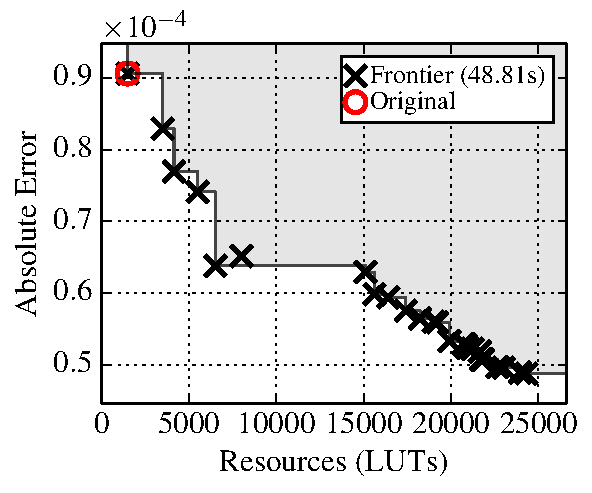
\includegraphics[width=0.6\linewidth]{euler}
        {}\label{fig:euler}
    } \\
    \subfloat[\texttt{filter}]{%
        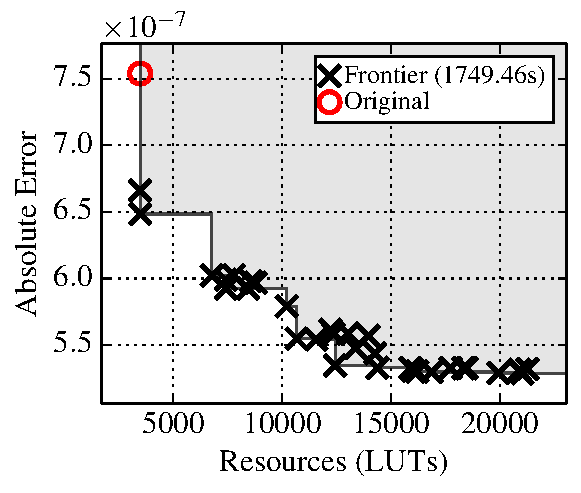
\includegraphics[width=0.6\linewidth]{filter}
        {}\label{fig:filter}
    }
    \caption{The Pareto frontier.}
\end{figure}

\section{Summary}
\label{so:sec:conclusion}

We provide a formal approach to the optimization of arithmetic expressions
for both accuracy and resource usage in high-level synthesis.  The method
proposed in this chapter and the associated tool, \soap, encompass three kind
of semantics that describe the accumulated roundoff errors, count operators in
expressions considering common subexpression elimination, and derive equivalent
expressions.  For a set of input expressions, the proposed approach works out
the respective sets of equivalent expressions in a hierarchical bottom-up
fashion, with a windowing depth limit and Pareto selection to help reduce the
complexity of equivalent expression discovery.  Using \soap, we improve either
the accuracy of our sample expressions or the resource utilization by up to
60\%, over the originals under single precision. \soap~enables a high-level
synthesis tool to optimize the structure as well as the precision of arithmetic
expressions, then to automatically choose an implementation that satisfies
accuracy and resource usage constraints.

Because we underpin our approach in formal semantics, it provides the
necessary foundation which permits us to extend the method for general
numerical program transformation in high-level synthesis.  Therefore in
Chapter~\ref{chp:progopt}, we base ourselves on the methodologies developed
in this chapter, and propose a structural approach to program optimization by
safely rewriting equivalent structures in numerical programs.



\chapter{Conclusion}
\label{chp:conclusion}

\section{Summary}
\label{so:sec:conclusion}

We provide a formal approach to the optimization of arithmetic expressions
for both accuracy and resource usage in high-level synthesis.  The method
proposed in this chapter and the associated tool, \soap, encompass three kind
of semantics that describe the accumulated roundoff errors, count operators in
expressions considering common subexpression elimination, and derive equivalent
expressions.  For a set of input expressions, the proposed approach works out
the respective sets of equivalent expressions in a hierarchical bottom-up
fashion, with a windowing depth limit and Pareto selection to help reduce the
complexity of equivalent expression discovery.  Using \soap, we improve either
the accuracy of our sample expressions or the resource utilization by up to
60\%, over the originals under single precision. \soap~enables a high-level
synthesis tool to optimize the structure as well as the precision of arithmetic
expressions, then to automatically choose an implementation that satisfies
accuracy and resource usage constraints.

Because we underpin our approach in formal semantics, it provides the
necessary foundation which permits us to extend the method for general
numerical program transformation in high-level synthesis.  Therefore in
Chapter~\ref{chp:progopt}, we base ourselves on the methodologies developed
in this chapter, and propose a structural approach to program optimization by
safely rewriting equivalent structures in numerical programs.


\cleardoublepage{}


% Back matter
{%
\setstretch{1.1}
\renewcommand{\bibfont}{\normalfont\small}
\setlength{\biblabelsep}{0pt}
\setlength{\bibitemsep}{0.5\baselineskip plus 0.5\baselineskip}
\printbibliography[]
}

% \input{colophon}
% \cleardoublepage

% \input{declaration}
% \clearpage
% \newpage
% \mbox{}

\begin{appendices}
    \bookmarksetupnext{level=-1}
    \addappheadtotoc%
    \makeatletter
    \addtocontents{toc}{\let\protect\l@chapter\protect\l@section}
    \makeatother
    \chapter{Sound Acceleration of Equivalent Expression Discovery}
\label{app:sound_acceleration}

The functions used in Section~\ref{so:sub:scalable} can sometimes be slow to
compute using a na\"ive implementation.  By using abstract interpretation and
the properties of certain \gls{eeg} functions, we can further accelerate the
computation.

We start by defining a property of the \gls{eeg} functions used in
Section~\ref{so:sub:scalable} known as \emph{$\cup$-distributive}, then propose
a new algorithm to accelerate the computation of $\closure_N f (\epsilon)$,
where $f$ is a $\cup$-distributive \gls{eeg}\@.
\begin{definition}
    We say an \gls{eeg} function $f$ is \emph{$\cup$-distributive} if and only
    if the function satisfies $f(\epsilon_a \cup \epsilon_b) = f(\epsilon_a)
    \cup f(\epsilon_b)$.
\end{definition}
\begin{corollary}
    By the definition of $\eqstep$ in~\eqref{so:eq:eqstep}, it is clear that
    $\eqstep$ is $\cup$-distributive.
    {}\label{so:cor:union}
\end{corollary}

Figure~\ref{so:alg:closure} proposes an accelerated algorithm to efficiently
compute $\closure_N f(\epsilon)$, where $f$ is a $\cup$-distributive
\gls{eeg}\@.
\begin{figure}[ht]
    \centering
    \begin{algorithmic}
        \Function{Closure}{$f$, $N$, $\epsilon$}
            \State{$s_0 \gets \epsilon$}
            \State{$s^\prime_0 \gets \epsilon$}
            \For{$i \gets 1, \ldots, N$}
                \State{$s^\prime_i \gets
                    f \left(s^\prime_{i-1}\right) - s_{i-1}$}
                \State{$s_i \gets s_{i-1} \cup s^\prime_i$}
                \If{$s^\prime_i = \emptyset$}
                    \State{\Return{$s_i$}}
                \EndIf{}
            \EndFor{}
            \State{\Return{$s_i$}}
        \EndFunction{}
    \end{algorithmic}
    \caption{%
        Our algorithm to compute $\closure_N f (\epsilon)$, which discovers a
        set of equivalent expressions with a $\cup$-distributive \gls{eeg} $f$
        from an initial set of equivalent expressions $\epsilon$.
    }\label{so:alg:closure}
\end{figure}

We then continue to prove that this algorithm $\textsc{Closure}(f, N,
\epsilon)$ indeed computes $\closure_N f(\epsilon)$.  Firstly, we prove the
following lemma:
\begin{lemma}
    $\closure_N f(\epsilon) = \epsilon \cup f \left( \closure_{N-1} f(\epsilon)
    \right)$ for any $\cup$-distributive \gls{eeg} function $f$.
    {}\label{so:lem:transitive}
\end{lemma}
\begin{proof}
    Following~\eqref{so:eq:transitive_generator}, $\closure_N f(\epsilon) =
    f^0(\epsilon) \cup f^1(\epsilon) \cup \cdots \cup f^N(\epsilon)$.  Because
    $f$ is $\cup$-distributive, we apply distributivity to the right-hand side
    to derive:
    \begin{equation}
        \closure_N f(\epsilon) = \epsilon \cup f\left(
            f^0(\epsilon) \cup f^1(\epsilon) \cup \cdots \cup f^{N-1}(\epsilon)
        \right),
    \end{equation}
    which equals to $\epsilon \cup f\left( \closure_{N-1} f(\epsilon) \right)$
    by definition.
\end{proof}
Then this allows us to deduce that the algorithm indeed computes $\closure_N
f(\epsilon)$:
\begin{theorem}
    In the algorithm in Figure~\ref{so:alg:closure}, at iteration $n$, the set
    of equivalent expressions $s_n$ computes exactly $\closure_n f(\epsilon)$,
    if $f$ is a $\cup$-distributive \gls{eeg}\@.
    \label{so:thm:closure}
\end{theorem}
\begin{proof}
    We start by assuming that at iteration $m > 0$, $s_m = \closure_m
    f(\epsilon)$, and we prove this equality still holds if substitute $m$ with
    $m + 1$.  From the algorithm, we can deduce:
    \begin{equation*}
        s_{m+1}
        = s_m \cup s^\prime_{m+1}
        = s_m \cup \left( f \left( s^\prime_m \right) - s_m \right)
        = s_m \cup f \left( s^\prime_m \right)
        = s_m \cup f \left(
            f \left( s^\prime_{m-1} \right) - s_{m-1}
        \right).
    \end{equation*}
    We substitute $s_m$ using Lemma~\ref{so:lem:transitive} to get:
    \begin{equation*}
        s_{m+1}
        = \epsilon \cup f \left( s_{m-1} \right) \cup
        f \left(
            f \left( s^\prime_{m-1} \right) - s_{m-1}
        \right).
    \end{equation*}
    Using distributivity of $f$ over $\cup$ and the iteration $m$ of the
    algorithm, we can derive:
    \begin{equation*}
        s_{m+1}
        = \epsilon \cup f \left(
            s_{m-1} \cup \left(
                f \left( s^\prime_{m-1} \right) - s_{m-1}
            \right)
        \right)
        = \epsilon \cup f \left( s_m \right).
    \end{equation*}
    Finally, we make use of the assumption $s_m = \closure_m f(\epsilon)$,
    followed by Lemma~\ref{so:lem:transitive} to show:
    \begin{equation*}
        s_{m+1}
        = \epsilon \cup f \left(
            \closure_m f(\epsilon)
        \right)
        = \closure_{m+1} f(\epsilon).
    \end{equation*}
    It is trivial that $s_0 = \epsilon = \closure_0 f(\epsilon)$, by induction,
    $s_n = \closure_n f(\epsilon)$ thus holds for all $n \in \naturalset$.
\end{proof}

Unfortunately, in the alternative method \greedytrace{}, we cannot make use of
the efficient algorithm in Figure~\ref{so:alg:closure} to compute $\closure_N
\left( \frontier \circ \eqstep_k \right)$ directly.  The reason is that in
general, $\frontier \circ \eqstep_k$ is not $\cup$-distributive.  Imagine two
equivalent expressions $e_1$ and $e_2$, and $e_1$ strictly dominates $e_2$,
\ie~$e_1$ is better than $e_2$ in terms of accuracy and resources, then we can
observe that:
\begin{equation}
    \frontier \left( \left\{ e_1 \right\} \cup \left\{ e_2 \right\} \right)
    = \frontier \left( \left\{ e_1, e_2 \right\} \right)
    = \left\{ e_1 \right\},
\end{equation}
which is not equal to:
\begin{equation}
    \frontier \left( \left\{ e_1 \right\} \right) \cup
    \frontier \left( \left\{ e_2 \right\} \right)
    = \left\{ e_1 \right\} \cup \left\{ e_2 \right\}.
\end{equation}

To resolve this, following \acrlong{ai} discussed in
Section~\ref{bg:sec:abstract_interpretation} of Chapter~\ref{chp:background},
we can introduce a new abstract domain to the power set of equivalent
expressions.  This new domain reduces the computation effort of equivalent
expression discovery, because it is a simpler domain with fewer elements than
the power set.

The abstract domain, represented by $\lattice{\absexprset}{\sqsubseteq}$, can
be inductively defined using the following Gal\"ois connection:
\begin{equation}
    \lattice{\eqexprpowerset}{\subseteq}
    \galois{\alpha}{\gamma}
    \lattice{\absexprset}{\sqsubseteq},
\end{equation}
where its abstraction and concretization functions are defined as follows:
\begin{equation}
    \begin{aligned}
        \alpha(\epsilon) &= \frontier(\epsilon), \quad
        \gamma(\epsilon^\sharp) &= \epsilon^\sharp.
    \end{aligned}
\end{equation}
Specifically, $\alpha$ is identical to $\frontier$, and $\gamma$ is simply the
identity function, \ie~it returns the input as its output.

The partial ordering on them ($\sqsubseteq$) and the join operator ($\sqcup$)
can then be defined inductively as follows using the Gal\"ois connection:
\begin{equation}
    \begin{aligned}
        \epsilon^\sharp_1 \sqsubseteq \epsilon^\sharp_2 &\defeq
            \left( \epsilon^\sharp_1 \sqcup \epsilon^\sharp_2 \right)
            = \epsilon^\sharp_2, \\
        \epsilon^\sharp_1 \sqcup \epsilon^\sharp_2 &\defeq
            \alpha\left(
                \gamma\left( \epsilon^\sharp_1 \right) \cup
                \gamma\left( \epsilon^\sharp_2 \right)
            \right).
    \end{aligned}
\end{equation}
Additionally, an abstract variant of an arbitrary \gls{eeg} $f$ can also be
inductively defined:
\begin{equation}
    f^\sharp (\epsilon^\sharp)
    = \alpha \circ f \circ \gamma \left(\epsilon^\sharp\right)
    = \frontier\left(f\left(\epsilon^\sharp\right)\right),
\end{equation}

Finally, the abstract variant of $\closure_N f$ can be proposed with a simple
modification to the algorithm in Figure~\ref{so:alg:closure}, by replacing
$\cup$ with $\sqcup$ in $s_i \gets s_{i-1} \cup s^\prime_i$, we now have
an abstract closure function:
\begin{equation}
    \closure^\sharp_N f^\sharp (\epsilon)
    = \bigsqcup_{n \in \naturalset} {f^\sharp}^n (\epsilon),
\end{equation}
that operates with an abstract \gls{eeg} $f^\sharp$.  The correctness of this
formulation can be proved by adapting Theorem~\ref{so:thm:closure} to the
modified algorithm.  The alternative method, \greedytrace{} which computes
$\closure^\sharp_N \eqstep_k^\sharp$, where $\eqstep_k^\sharp = \frontier \circ
\eqstep_k$ can finally be accelerated using the modified algorithm.  Moreover,
the discovery is further accelerated with the new algorithm because of the
property:
\begin{equation}
    f^\sharp\left(\epsilon^\sharp_1 \sqcup \epsilon^\sharp_2\right)
    \sqsubseteq f^\sharp\left(\epsilon^\sharp_1\right)
    \sqcup f^\sharp\left(\epsilon^\sharp_2\right).
\end{equation}

    \chapter{Formal Definitions of Equivalent MIR Discovery}
\label{app:formal}

In Section~\ref{po:sec:equivalence_analysis} of Chapter~\ref{chp:progopt}
informally explained how equivalent semantic expressions and
\glspl{mir} can be discovered.  In this appendix we formally define the
equivalent discovery procedure for all newly introduced operators in
Section~\ref{po:sec:program_to_mir}, \ie~the ternary conditional, composition,
and fixpoint operators, and also extend this definition to \glspl{mir} in a
similar fashion.

Formally, we extend the optimization function $\optfunc{\cdot}: M \to
\errordom \to M$, where $M = \sexprset \cup \mirset$, proposed in
Section~\ref{so:sec:equivalent} of Chapter~\ref{chp:stropt} to these above
structures.  For ternary conditional operators, we have:
\begin{equation}
    \optfunc{\ternarymir{$\qop$}{$b$}{$e_1$}{$e_2$}}\sigma^\sharp
    = f_{\sigma^\sharp} \left( \left\{
        \ternarymir{$\qop$}{$b^\prime$}{$e^\prime_1$}{$e^\prime_2$}
        \left|
        \tikz[baseline=(current bounding box.center), text height=0]{%
            \node at (0, 0) {%
                $b^\prime \in \optfunc{b}\sigma^\sharp,$
            };
            \node at (1.8mm, -5mm) {%
                $e^\prime_1 \in \optfunc{e_1}\sigma^\sharp|_b^\prime,$
            };
            \node at (1.5mm, -10mm) {%
                $e^\prime_2 \in \optfunc{e_2}\sigma^\sharp|_b^\prime$
            };
        }
        \right.
    \right\} \right),
\end{equation}
where the function $f_{\sigma^\sharp}$ is defined in
Section~\ref{so:sub:equivalent_semantics} of Chapter~\ref{chp:stropt}.

Similarly, the function can also be defined for the composition operator:
\begin{equation}
    \optfunc{\binarymir{$\expand$}{$e$}{$\mu$}}\sigma^\sharp
    = \frontier\left( \left\{
        \left.
            \binarymir{$\expand$}{$e^\prime$}{$\mu^\prime$}
        \right|
        \tikz[baseline=(current bounding box.center), text height=1mm]{%
            \node at (0, 0) {%
                $e^\prime \in \optfunc{e} \left(
                    \mirerrorfunc{\mu^\prime}\sigma^\sharp
                \right),$

            };
            \node at (0mm, -6mm) {%
                $\mu^\prime \in \optfunc{\mu}\sigma^\sharp$
            };
        }
    \right\}, \sigma^\sharp \right),
\end{equation}
where $\frontier\left(\epsilon, \sigma^\sharp\right)$ computes the
Pareto-optimal set of equivalent semantic expressions from the initial set
$\epsilon$, using the program state $\sigma^\sharp$ to evaluate the quality
metrics (\ie~round-off errors and resource utilization).

In addition, a formal mathematical definition of the process of discovering
equivalent fixpoint expressions is:
\begin{equation}
    \optfunc{
        \fixpointmir{$b$}{$\mu$}{\varx}
    }\sigma^\sharp
    = \frontier \left( \left\{
        \fixpointmir{$b^\prime$}{$\mu^\prime$}{\varx}
        \left|
        \tikz[baseline=(current bounding box.center), text height=5mm]{%
            \node at (0, 0) {%
                $\loopinvar = \mathsf{E}_\mathsf{s}^\mathrm{LI} \left[
                    \fixpointmir{$b$}{$\mu$}{\varx}
                \right]\sigma^\sharp,$
            };
            \node at (0, -9mm) {%
                $b^\prime \in \optfunc{b}\loopinvar,$
            };
            \node at (0, -19mm) {%
                $\displaystyle \mu^\prime \in \bigcup_{k=0}^{K}
                \optfunc{p^k_\mu (\mu)}\loopinvar$
            };
        }
        \right.
    \right\}, \sigma^\sharp \right),
\end{equation}
where $K$ is the partial unroll factor limit.  We set $K = 3$ in the
experimental results discussed in Section~\ref{po:sec:results}.

Finally, \glspl{mir} can also be optimized in a similar fashion, by
recursively discovering equivalent expressions within it:
\begin{equation}
    \optfunc{\mu}\sigma^\sharp = \frontier\left( \left\{
        {\left[ \varx \mapsto e_\varx \right]}_{\varx \in \varfunc{\mu}}
        \left|
        \tikz[baseline=(current bounding box.center), text height=1mm]{%
            \node at (0, 0) {%
                $e_\vary \in \optfunc{\mu(\vary)}\sigma^\sharp,$

            };
            \node at (0mm, -6mm) {%
                $\vary \in \varfunc{\mu}$
            };
        }
        \right.
    \right\}, \sigma^\sharp \right).
\end{equation}

    \chapter{Benchmark Source Code}
\label{app:source}

In Chapters~\ref{chp:progopt} and~\ref{chp:latopt} we explore the experimental
results of several numerical programs as our benchmark examples.  This appendix
contains the source code of the benchmark suite used.

\begin{figure}[ht]
\begin{lstlisting}
#pragma soap in float x=[0, 20]
#pragma soap out x

while (x > 1.0) {
    x = 0.9f * x;
}
\end{lstlisting}
\caption{\texttt{simple}}
\end{figure}

\begin{figure}[ht]
\begin{lstlisting}
#pragma soap in \
    int n=[10, 20], float x=[-0.1, 0.1], float y=[0, 1]
#pragma soap out z

float a = 1;
int b = 1;
float p = 1;
float z = 0.0f;
for (int i = 0; i < n; i++) {
    a = -a;
    b *= (2 * i + 1) * (2 * i);
    p *= (x + y) * (x + y);
    z += (a / b) * p;
}
\end{lstlisting}
\caption{\texttt{taylor}}
\end{figure}

\begin{figure}[ht]
\begin{lstlisting}
#pragma soap in \
    float a0=[0, 0.2], float a1=[0, 0.2], \
    float a2=[0.0, 0.2], float b0=[0, 0.2], \
    float b1=[0, 0.2], float b2=[0.0, 0.2], \
    float x=[0, 1], int n=20
#pragma soap out y

float x1 = 0.0f, x2 = 0.0f;
float y1 = 0.0f, y2 = 0.0f;
float y = x;
for (int i = 0; i < n; i++) {
    float yt = y;
    y = b0 * x + b1 * x1 + b2 * x2 +
        a0 * y + a1 * y1 + a2 * y2;
    x2 = x1;
    x1 = x;
    y2 = y1;
    y1 = yt;
}
\end{lstlisting}
\caption{\texttt{filter}}
\end{figure}

\begin{figure}[ht]
\begin{lstlisting}
#pragma soap in \
    float u=[0.0, 1.0], float w=[0.0, 1.0], \
    int n=[0, 20], float dt=[0.1, 0.1]
#pragma soap out u, v

float u;
float v = 0.0f;
for (int i = 0; i < n; i++) {
    float u0 = u + v * dt;
    v -= w * u * dt;
    u = u0;
}
\end{lstlisting}
\caption{\texttt{euler}}
\end{figure}

\begin{figure}[ht]
\begin{lstlisting}
#define n 20
#pragma soap in \
    float kp=[9, 10], float ki=[0.5, 0.7], float kd=[0, 3], \
    float dt=[0.2, 0.2], float m=8.0, float c=5.0,
#pragma soap out m

float i = 0.0f, e0 = 0.0f;
float m, e, d, r;
for (int j = 0; j < n; j++) {
    e = c - m;
    i += ki * dt * e;
    d = kd * (e - e0) / dt;
    r = kp * e + i + d;
    e0 = e;
    m += 0.01f * r;
}
\end{lstlisting}
\caption{\texttt{pid}}
\end{figure}


\begin{figure}[ht]
\begin{lstlisting}
#define N 4096
#pragma soap in float x[N] = [0.0, 1.0]
#pragma soap out sum

float sum = 0;
for (int i = 0; i < N; i = i + 1) {
    sum = sum + x[i];
}
\end{lstlisting}
\caption{\texttt{sum}}
\end{figure}


\begin{figure}[ht]
\begin{lstlisting}
#define N 4096
#pragma soap in \
    float x[100] = [0.0, 1.0], float z[100] = [0.0, 1.0]
#pragma soap out q

float q = 0.0f;
for (int k = 0; k < N; k++) {
    q = q + z[k] * x[k];
}
\end{lstlisting}
\caption{\texttt{dotprod}}
\end{figure}


\begin{figure}[ht]
\begin{lstlisting}
#define loop 1024
#define n 1024
#pragma soap in \
    float x[n] = [0.0, 1.0], float y[n] = [0.0, 1.0], \
    float z[n] = [0.0, 1.0]
#pragma soap out x

int l; int i;
for ( l=1 ; l<=loop ; l++ ) {
    for ( i=1 ; i<n ; i++ ) {
        x[i] = z[i]*( y[i] - x[i-1] );
    }
}
\end{lstlisting}
\caption{\texttt{tridiag}}
\end{figure}


\begin{figure}[ht]
\begin{lstlisting}
// D := alpha*A*B*C + beta*D

#define N 1024
#pragma soap in \
    float A[N][N] = [0.0, 1.0], float B[N][N] = [0.0, 1.0], \
    float C[N][N] = [0.0, 1.0], float D[N][N] = [0.0, 1.0], \
    float tmp[N][N] = [0.0, 1.0]
#pragma soap out D

int i; int j; int k;
float alpha = 32412;
float beta = 2123;
for (i = 0; i < N; i++)
    for (j = 0; j < N; j++) {
        tmp[i][j] = 0;
        for (k = 0; k < N; ++k)
            tmp[i][j] += alpha * A[i][k] * B[k][j];
    }
for (i = 0; i < N; i++)
    for (j = 0; j < N; j++) {
        D[i][j] *= beta;
        for (k = 0; k < N; ++k)
            D[i][j] += tmp[i][k] * C[k][j];
    }
\end{lstlisting}
\caption{\texttt{2mm}}
\end{figure}


\begin{figure}[ht]
\begin{lstlisting}
// G = (A * B) * (C * D)
#define N 1024
#pragma soap in \
    float A[N][N] = [0.0, 1.0], float B[N][N] = [0.0, 1.0], \
    float C[N][N] = [0.0, 1.0], float D[N][N] = [0.0, 1.0], \
    float E[N][N] = [0.0, 1.0], float F[N][N] = [0.0, 1.0], \
    float G[N][N] = [0.0, 1.0]
#pragma soap out G

int i; int j; int k;
for (i = 0; i < N; i++) /* E := A*B */
    for (j = 0; j < N; j++) {
        E[i][j] = 0;
        for (k = 0; k < N; ++k)
            E[i][j] += A[i][k] * B[k][j];
    }
for (i = 0; i < N; i++) /* F := C*D */
    for (j = 0; j < N; j++) {
        F[i][j] = 0;
        for (k = 0; k < N; ++k)
            F[i][j] += C[i][k] * D[k][j];
    }
for (i = 0; i < N; i++) /* G := E*F */
    for (j = 0; j < N; j++) {
        G[i][j] = 0;
        for (k = 0; k < N; ++k)
            G[i][j] += E[i][k] * F[k][j];
    }
\end{lstlisting}
\caption{\texttt{3mm}}
\end{figure}


\begin{figure}[ht]
\begin{lstlisting}
#define N 4000
#pragma soap in \
    float A[N][N] = [0.0, 1.0], float x[N] = [0.0, 1.0], \
    float y[N] = [0.0, 1.0], float tmp[N] = 0
#pragma soap out y

int i; int j;
for (i = 0; i < N; i++) {
    tmp[i] = 0;
    for (j = 0; j < N; j++)
        tmp[i] = tmp[i] + A[i][j] * x[j];
    for (j = 0; j < N; j++)
        y[j] = y[j] + A[i][j] * tmp[i];
}
\end{lstlisting}
\caption{\texttt{atax}}
\end{figure}


\begin{figure}[ht]
\begin{lstlisting}
#define N 4000
#pragma soap in \
    float A[N][N] = [0.0, 1.0], float s[N] = [0.0, 1.0], \
    float q[N] = 0, \
    float p[N] = [0.0, 1.0], float r[N] = [0.0, 1.0]
#pragma soap out q

int i; int j;
for (i = 0; i < N; i++)
    s[i] = 0;
for (i = 0; i < N; i++)
{
    q[i] = 0;
    for (j = 0; j < N; j++)
    {
        s[j] = s[j] + r[i] * A[i][j];
        q[i] = q[i] + A[i][j] * p[j];
    }
}
\end{lstlisting}
\caption{\texttt{bicg}}
\end{figure}


\begin{figure}[ht]
\begin{lstlisting}
// C := alpha*A*B + beta*C
#define N 1024
#pragma soap in \
    float C[N][N] = [0.0, 1.0], float A[N][N] = [0.0, 1.0], \
    float B[N][N] = [0.0, 1.0]
#pragma soap out C

int i; int j; int k;
float alpha = 32412;
float beta = 2123;
for (i = 0; i < N; i++)
    for (j = 0; j < N; j++) {
        C[i][j] *= beta;
        for (k = 0; k < N; ++k)
            C[i][j] += alpha * A[i][k] * B[k][j];
    }
\end{lstlisting}
\caption{\texttt{gemm}}
\end{figure}


\begin{figure}[ht]
\begin{lstlisting}
// Vector Multiplication and Matrix Addition
#define N 1024
#pragma soap in \
    float A[N][N] = [0.0, 1.0], \
    float u1[N] = [0.0, 1.0], float v1[N] = [0.0, 1.0], \
    float u2[N] = [0.0, 1.0], float v2[N] = [0.0, 1.0], \
    float w[N] = 0, float x[N] = 0, \
    float y[N] = [0.0, 1.0], float z[N] = [0.0, 1.0]
#pragma soap out w

int i; int j;
float alpha = 43532;
float beta = 12313;
for (i = 0; i < N; i++)
    for (j = 0; j < N; j++)
        x[i] = x[i] + beta * A[j][i] * y[j];
for (i = 0; i < N; i++)
    x[i] = x[i] + z[i];
for (i = 0; i < N; i++)
    for (j = 0; j < N; j++)
        w[i] = w[i] +  alpha * A[i][j] * x[j];
\end{lstlisting}
\caption{\texttt{gemver}}
\end{figure}


\begin{figure}[ht]
\begin{lstlisting}
// Matrix Vector Product and Transpose
#define N 1024
#define N 1024
#pragma soap in \
    float x1[N] = [0.0, 1.0], float x2[N] = [0.0, 1.0], \
    float y_1[N] = [0.0, 1.0], float y_2[N] = [0.0, 1.0], \
    float A[N][N] = [0.0, 1.0]
#pragma soap out x1, x2

int i; int j;
for (i = 0; i < N; i++)
    for (j = 0; j < N; j++)
        x1[i] = x1[i] + A[i][j] * y_1[j];
for (i = 0; i < N; i++)
    for (j = 0; j < N; j++)
        x2[i] = x2[i] + A[j][i] * y_2[j];
\end{lstlisting}
\caption{\texttt{mvt}}
\end{figure}


\begin{figure}[ht]
\begin{lstlisting}
#define N 1000
#define TSTEPS 20
#pragma soap in float A[N][N] = [0.0, 1.0]
#pragma soap out A

int t; int i; int j;
for (t = 0; t < TSTEPS; t++)
    for (i = 1; i < N - 1; i++)
        for (j = 1; j < N - 1; j++)
            A[i][j] = (A[i-1][j]
        + A[i][j-1] + A[i][j] + A[i][j+1] + A[i+1][j]) * 0.2f;
\end{lstlisting}
\caption{\texttt{seidel}}
\end{figure}


\begin{figure}[ht]
\begin{lstlisting}
// Symmetric rank-2k operations
#define N 1024
#pragma soap in \
    float alpha = [0.0, 1.0], float beta = [0.0, 1.0], \
    float A[N][N] = [0.0, 1.0], float B[N][N] = [0.0, 1.0], \
    float C[N][N] = [0.0, 1.0]
#pragma soap out C

int i; int j; int k;
for (i = 0; i < N; i++)
    for (j = 0; j < N; j++)
        for (k = 0; k < N; k++) {
            C[i][j] += alpha * A[i][k] * B[j][k];
            C[i][j] += alpha * B[i][k] * A[j][k];
        }
\end{lstlisting}
\caption{\texttt{syr2k}}
\end{figure}

\end{appendices}

\end{document}
